\chapter{Quantum computation}\label{ch:qc}

Quantum computing dates back to 1982 when the Nobel laureate Richard Feynman proposed the idea of constructing computers based on quantum mechanics principles to efficiently simulate quantum phenomena \cite{feynman2018simulating}. 
The field has since evolved into a multidisciplinary research area that combines quantum mechanics, computer science, and information theory. Quantum information theory, in particular, is based on the idea that if there are new physics laws, there should be new ways to process and transmit information.  In classical information theory, all systems (computers, communication channels, etc.) are fundamentally equivalent, meaning they adhere to consistent scaling laws. These laws, therefore, govern the ultimate limits of such systems. For instance, if the time required to solve a particular problem, such as the factorization of a large number, increases exponentially with the size of the problem, this scaling behavior remains true irrespective of the computational power available.  Such a problem, growing exponentially with the size of the object, is known as a ``difficult problem". However, as demonstrated by Peter Shor, the use of a quantum computer with a sufficient number of quantum bits (qubits) could significantly accelerate the factorization of large numbers \cite{shor1994algorithms}.  This advancement poses a significant threat to the security of confidential data transmitted over the Internet, as the RSA algorithm is based on the computational difficulty of factorizing large numbers. This result underscores the promise of the quantum computing paradigm.


\paragraph{Quantum computing and the need for quantitative reasoning.}
%The quantum computing paradigm holds immense promise, as evidenced by this compelling result in computational complexity theory.  
While hardware advancements have brought the scientific community closer to realizing the transformative potential of quantum computing, the ultimate goal is yet to be accomplished. A NISQ computer equipped with 50-100 qubits may surpass the capabilities of current classical computers, yet the impact of quantum noise, such as decoherence in entangled states, imposes limitations on the size of quantum circuits that can be executed reliably \cite{preskill2018quantum}. Unfortunately, general-purpose error correction techniques \cite{calderbank1996good, gottesman1997stabilizer, steane1996error} consume a substantial number of qubits, making it difficult for NISQ devices to make use of them in the near term. For instance, the implementation of a single logical qubit may require between $10^3$ and $10^4$ physical qubits \cite{fowler2012surface}. As a result, it is unreasonable to expect that the idealized quantum algorithm will run perfectly on a quantum device, instead, only a mere approximation will be observed.

To reconcile quantum computation with NISQ computers, quantum compilers perform transformations for error mitigation \cite{wallman2016noise} and noise-adaptive optimization \cite{murali2019noise}. Additionally, current quantum computers only support a restricted, albeit universal, set of quantum operations. As a result, non-native operations must be decomposed into sequences of native operations before execution \cite{harrow2002efficient,burgholzer2020advanced}. The assessment of these compiler transformations necessitates a comparison of the error bounds between the source and compiled quantum programs, which calls for the development of appropriate notions of approximate program equivalence.


%Furthermore, in quantum information theory, the concept of an $\epsilon-\text{approximation}$ channel is fundamental when studying quantum teleportation via noisy channels \cite{watrous2018theory}. 

As previously noted, Shor's algorithm has played a pivotal role in sparking heightened interest within the scientific community towards quantum computing research. Several quantum programming languages have surfaced over the past 25 years \cite{zhao2020quantum,serrano2022quantum}. Among them, we highlight Selinger's and Valirion's work. In 2004, Selinger introduced a first-order functional language for quantum computation, QPL, along with its denotational semantics \cite{selinger2004towards}. Building on this, Selinger and Valiron later developed a higher-order functional language for quantum computation—commonly referred to as a quantum lambda calculus. They first presented a version with classical control and its operational semantics in \cite{selinger2006lambda}. This was followed by a denotational semantics for a fragment of the language in \cite{selinger2008fully}. In subsequent work, they extended the quantum lambda calculus to include recursion and infinite types, along with its operational semantics \cite{selinger2009quantum}. Later, they proposed an alternative approach to its denotational semantics \cite{selinger2014}.


These works adopt Schr\"odinger's picture, in which quantum programs are interpreted as maps between quantum states (\ie, density operators). In contrast, \cite{choSemanticsQuantumProgramming2016, choNeumannAlgebrasForm2016} consider Heisenberg's picture, in which programs are modeled as maps between observables (\ie, self-adjoint operators). Particularly, \cite{choSemanticsQuantumProgramming2016} presents a model based on $W^*$-algebras, which can be viewed as an infinite-dimensional extension of \cite{selinger2004towards}. Moreover, \cite{choSemanticsQuantumProgramming2016} presents a model of Selinger and Valiron’s quantum lambda calculus \cite{selinger2006lambda, selinger2008linear, selinger2009quantum}, also based on $W^*$-algebras, and proves the model's adequacy.


Most of the current research on algorithms and programming languages assumes that addressing the challenge of noise during program execution will be resolved either by the hardware or through the implementation of fault-tolerant protocols designed independently of any specific application \cite{chong2017programming}. As previously stated, this assumption is not realistic in the NISQ era. Nonetheless, there have been efforts to address the challenge of approximate program equivalence in the quantum setting. For example, \cite{hung2019quantitative} and \cite{tao2021gleipnir} reason about the issue of noise in a quantum while-language by developing a deductive system to determine how similar a quantum program is from its idealised, noise-free version. The former introduces the ($Q$,$\lambda$)-diamond norm, which analyzes the output error given that the input quantum state satisfies some quantum predicate $Q$ to degree $\lambda$. However, it does not specify any practical method for obtaining non-trivial quantum predicates. In fact, the methods used in \cite{hung2019quantitative} cannot produce any post conditions other than $(I,0)$ (\textit{i.e.}, the identity matrix $I$ to degree 0, analogous to a ``true” predicate) for large quantum programs. The latter specifically addresses and delves into this aspect.  

An alternative approach was explored in \cite{dahlqvist2023syntactic}, using linear $\lambda$-calculus as basis. A notion of approximate equivalence is then
integrated in the calculus via the so-called diamond norm, which induces a metric on the space of quantum programs (seen semantically as completely positive trace-preserving super-operators) \cite{watrous2018theory}. 


\vspace{20pt}

The first two sections of this chapter present  mathematical and quantum computing preliminaries necessary for understanding the theory of quantum computation. This introduction to quantum computing draws primarily from \cite{nielsen2010quantum,watrous2018theory}, while the mathematical foundations are also based on \cite{heinosaariMathematicalLanguageQuantum2011,conwayCourseFunctionalAnalysis2007,conwayCourseOperatorTheory2000}.
The next section introduces core concepts from functional analysis that are essential for understanding \( W^* \)-algebras, based on \cite{rudin91functional,guide2006infinite}. This is followed by a section presenting the fundamentals of \( W^* \)-algebras, drawing primarily from \cite{sakaiCAlgebrasWAlgebras1998,takesakiTheoryOperatorAlgebras1979,westerbaanCategoryNeumannAlgebras2019}.
We then show that both Selinger’s category 
$\catQ$ of quantum operations (i.e., completely positive, trace-nonincreasing super-operators) \cite{selinger2004towards}, and Cho’s category 
$\WstarCPSUop$, the opposite category of \( W^* \)-algebras with normal, completely positive, subunital maps \cite{choSemanticsQuantumProgramming2016}, are first-order models of our calculus.
Finally, the last section provides a few illustrative examples in the setting of quantum information.







\section{Hilbert Spaces} \label{sec:linalg}



It is impossible to present the theory of quantum computation without introducing some concepts of theory of Hilbert spaces and operators. This section briefly overwiews of the aspects of Hilbert spaces that are most pertinent to the study of quantum computation. 

\begin{convention}
  In this section and the one that follows, vector spaces are assumed to be finite-dimensional, unless otherwise stated.
\end{convention}



%The letters \gls{vectorspaces} will often be used to refer to vector spaces. In this section, all vector spaces are assumed to be finite dimensional, unless otherwise stated.



\begin{comment}

  \subsection{Vector spaces}

The basic objects of linear algebra are vector spaces. The vector spaces of interest in this work are the real and complex vector spaces, such as  \gls{real-space}  and \gls{n-complex-space} and \gls{matrix-complex-space}, respectively. 

\begin{definition}
A \emph{vector space} (over a field $\mathcal{F}$)  consists of a set $V$ whose elements are called vectors, together with two operations:
\begin{itemize}
  \item An operation called vector addition that takes two vectors $v, w \in V$ , and results in a third vector, written $v + w \in V$;
  \item An operation called scalar multiplication that takes a scalar $a \in \mathcal{F}$ and a vector $v \in V,$  and results in a new vector, written $a \cdot v \in V$
\end{itemize}
which satisfy the following axioms, for all $u, v, w \in V$ and $a_1, a_2 \in \mathcal{F}$:

\begin{enumerate}
  \item Vector addition is commutative: $u + v = v + u$;
  \item Vector addition is associative: $(u + v) + w = u + (v + w) $;
  \item There is a zero vector $0 \in V$ such that $v +0 = v$ for all $v \in V$;
  \item Each $v \in V$ has an additive inverse $w \in V$ such that $w + v = 0$;
  \item Scalar multiplication distributes over scalar addition, $(a_1+a_2) \cdot v = a_1 \cdot v + a_2 \cdot v$;
  \item Scalar multiplication distributes over vector addition, $a_1 \cdot (v + w) = a_1 \cdot v + a_1 \cdot w$;
  \item Ordinary multiplication of scalars associates with scalar multiplication, $(a_1 a_2) \cdot v = a_1 \cdot (a_2 \cdot v)$;
  \item Multiplication by the scalar 1 is the identity operation, $1 \cdot v = v$.
\end{enumerate}

\end{definition}

 

The letters \gls{vectorspaces} will often be used to refer to vector spaces. In this section, all vector spaces are assumed to be finite dimensional, unless otherwise stated.  

\begin{comment}

In the case of the vector space $\mathbb{C}^{n}$, the space of all n-tuples of complex numbers, $(a_1, \ldots , a_n)$, addition and scalar multiplication are defined in the following standard way:
\begin{itemize}
  \item Addition: for vectors $u = (a_1, \ldots , a_n), v = (b_1, \ldots , b_n)  \in \mathbb{C}^{n}$, the vector $u + v \in \mathbb{C}^{n}$ is defined by the equation $(u + v) = (a_1 + b_1, \ldots, a_n+b_n)$.
  \item Scalar multiplication: for a scalar $a \in \mathbb{C}$ and a vector $v = (b_1, \ldots , b_n) \in \mathbb{C}^{n}$, the vector $a \cdot v \in \mathbb{C}^{n}$ is defined by the equation $a \cdot v = (a \cdot b_1, \ldots, a \cdot b_n)$.
\end{itemize}
The zero vector in $\mathbb{C}^{n}$ is the vector with all entries equal to zero.

Sometimes, the column matrix notation is used to represent vectors in $\mathbb{C}^{n}$, that is, a vector $v \in \mathbb{C}^{n}$ is written as a column matrix $$v = \begin{pmatrix} a_1 \\ \vdots \\ a_n \end{pmatrix}.$$ Other times for readability the format $(a_1, \ldots , a_n)$ is used. The latter should be interpreted as a shorthand for a column vector.

$\mathbb{C}^{n \times m}$ is a vector space when addition is defined as matrix addition and scalar multiplication is defined as multiplication of each component by the scalar. The zero vector is the zero matrix, \textit{i.e.}, the matrix with all entries equal to zero.

%p.240 linear algebra 
%\begin{theorem} \label{theorem:dist_matrix} \cite{hefferon2006linear}
  %If $A, B, C$ are matrices, and the matrix products are defined,
%then the product is associative $(AB)C = A(BC)$ and distributes over matrix
%addition $A(B + C) = AB + AC$ and $(B + C)A = BA + CA$.


\begin{definition}
A \emph{vector subspace} of a vector space $V$ is a subset $W$ of $V$ such that $W$ is also a vector space, that is, $W$ must be closed under scalar multiplication and addition.
\end{definition}
%\end{theorem}


\begin{definition}
  A \emph{spanning set} of a vector space is a set of vectors $v_{1}, \ldots, v_{n}$ such that any vector $v$ in the vector space can be written as a linear combination $v = \sum_{i} a_{i} v_{i}$ of vectors in that set, where $a_{i}$ are scalars.
\end{definition}


\begin{definition}
A set of non-zero vectors $v_1, \ldots, v_n$ are \emph{linearly dependent} if there exists a set of complex numbers $a_1, \ldots , a_n$ with $a_i \neq 0$ for at least one value of $i$, such that
\begin{equation*}
  a_1 v_1 + a_2 v_2 +\ldots a_n v_n = 0.
\end{equation*}
\end{definition}

\begin{definition}
A set of vectors $v_1, \ldots, v_n$ are \emph{linearly independent} if they are not linearly dependent.
\end{definition}

\begin{definition}
A \emph{basis} for a vector space is a sequence of vectors that is linearly
independent and that spans the space.
\end{definition}

\begin{definition}
The number of elements in the basis is defined to be the \emph{dimension}  of
$V$, denoted \gls{dim}.
\end{definition}





\subsection{Linear operators}

\begin{definition}
  A \emph{linear operator} between vector spaces $V$ and $W$ is defined to be any function $A : V \rightarrow W$ which is linear in its inputs, \textit{i.e.}
\begin{equation*}
  A \left( \sum_{i} a_{i} v_{i} \right) = \sum_{i} a_i A (v_{i})
\end{equation*}
\end{definition}

Usually $A(v)$ is just denoted $A v$.

Suppose $V, W,$ and $R$ are vector spaces, and $A : V \rightarrow R$ and $B : W \rightarrow R$ are linear operators. Then the notation $BA$ is used  to denote the \emph{composition} of $B$ with $A$,
defined by $(BA)(v) \equiv B(A(v))$. Once again, $(BA)(v)$ is abbreviated as  $BA \hspace{1pt}v$.

For any choice of complex spaces $V \in \mathbb{C}^n $ and $W \in \mathbb{C}^m$, there is a bijective linear correspondence between the set of operators from $V$ to $W$ and the set of $n \times m$ matrices. %To see the connection, it helps to first understand that an $m$ by $n$ complex matrix $A$ with entries $A_{ij}$ is in fact a linear operator sending vectors in the vector space $\mathbb{C}^n$ to the vector space $\mathbb{C}^m$, under matrix multiplication of the matrix $A$ by a vector in $\mathbb{C}^n$. Nevertheless, this matrix can also be seen as an a linear operator sending vectors in the vector space $\mathbb{C}^{n \times p}$ to the vector space $\mathbb{C}^{m \times p}$, under matrix multiplication of the matrix $A$ by a matrix in $\mathbb{C}^{n \times p}$. 
The claim that the matrix $A \in \mathbb{C}^{m\times n}$ is a linear operator just means that
\begin{equation*}
  A \left( \sum_{i} a_{i} v_{i} \right) = \sum_{i} a_i A (v_{i})
\end{equation*}
is true as an equation where the operation is matrix multiplication of $A$ by a collumn vector in $\mathbb{C}^n$. Clearly, this is true! On the other hand, suppose $A : V \rightarrow W$ is a linear operator between vector spaces $V$ and $W$, such that $V \in \mathbb{C}^n $ and $W \in \mathbb{C}^m$. Suppose $v_1,\ldots, v_n$ is a basis for $V$ and $w_1,\ldots,w_n $ is a
basis for $W$. Then for each $j$ in the range $1, \ldots ,m$, there exist complex numbers $A_{1j}$ through $A_{nj}$ such that
\begin{equation*}
  A \hspace{1pt} v_j = \sum_{i} A_{ij} w_i.
\end{equation*}
The matrix whose entries are the values $A_{ij}$ is said to form a \emph{matrix representation} of the operator $A$. This matrix representation of $A$ is completely equivalent to the operator $A$. As a result, when considering operators on vector spaces of the form $\mathbb{C}^n$ it is common to refer to the operator $A$ and its matrix representation interchangeably.

%The claim that the matrix $A \in \mathbb{C}^{m\times n}$ is a linear operator just means that
%\begin{equation*}
 % A \left( \sum_{i} a_{i} v_{i} \right) = \sum_{i} a_i A (v_{i})
%\%end{equation*}
%is true as an equation where the operation is matrix multiplication of $A$ by a collumn vector in $\mathbb{C}^n$ or by a matrix in $\mathbb{C}^{n \times p}$. Clearly, this is true! On the other hand, suppose $A : V \rightarrow W$ is a linear operator between vector spaces $V$ and $W$, such that $V \in \mathbb{C}^m $ and $W \in \mathbb{C}^m$ or $V \in \mathbb{C}^{n\times p} $ and $W \in \mathbb{C}^{m\times p}$. Suppose $v_1,\ldots, v_n$ is a basis for $V$ and $w_1,\ldots,w_n $ is a
%basis for $W$. Then for each $j$ in the range $1, \ldots ,m$, there exist complex numbers $A_{1j}$ through $A_{nj}$ such that
%\begin{equation*}
  %A \hspace{1pt} v_j = \sum_{i} A_{ij} w_i.
%\end{equation*}
%The matrix whose entries are the values $A_{ij}$ is said to form a \emph{matrix representation} of the operator $A$. This matrix representation of $A$ is completely equivalent to the operator $A$. As a result, when considering operators on vector spaces of the form $\mathbb{C}^n$ or $\mathbb{C}^{n\times n}$, it is common to refer to the operator $A$ and its matrix representation interchangeably.

\end{comment}


\subsection{Inner product}
%When refering to the vector product in an arbitrary vector space, the notation \gls{inner-product} will be used.



\begin{definition} \label{def:inner_product}
An \emph{inner product}~\gls{inner-product} on a vector space $V$ is a function from a mapping $V\times V$ to the field of scalars, $\langle \cdot, \cdot \rangle : V \times V \rightarrow \mathbb{C}$,  that satisfies the following properties for all $v, w, w_1, \ldots, w_n \in V$ and $\alpha_1, \ldots, \alpha_n \in \mathbb{C}.$

\begin{enumerate}
  \item Linearity in the second argument,$$ \left\langle v, \sum_{i=1}^n \alpha_i w_i\right\rangle = \sum_{i=1}^n \alpha_i \langle v, w_i\rangle. $$
  \item $\langle v,w \rangle = \overline{\langle w,v \rangle} $, \text{  where \gls{conj} is the complex conjugate operation.}
  \item  $\langle v,w \rangle \geq 0 $ with equality if and only if $v = 0$.
\end{enumerate}
\end{definition}

\begin{example}
  For instance, the inner product $ \langle v, w \rangle$ of two vectors $ v = (\alpha_1, \ldots, \alpha_n ),w = (\beta_1, \ldots, \beta_n) \in \mathbb{C}^{n}$ is defined as
\begin{equation*}
  \langle v, w \rangle = \sum_{i} \overline{\alpha}_i \beta_i. 
\end{equation*}
\end{example}


Every inner product space is a normed space, where the norm of a vector $v \in V$ is defined as $\|v\| = \sqrt{\langle v, v \rangle}$.


\begin{definition}
  A \emph{Hilbert space} $\mathcal{H}$ is an inner product space.
\end{definition}


The letters \gls{hilbertspaces} will often be used to refer to Hilbert spaces.

\begin{definition} \label{def:positive}
  \emph{Positive (semidefinite) operators}. A square operator $A\in \mathcal{B}(\HilbH)$ is \emph{positive}, denoted $A \geq 0$, if $\langle v, Av \rangle \geq 0$ for all $v \in  \mathcal{B}(\HilbH)$.    
  %sum ->p.163 theory of quantum information
\end{definition}



\subsection{Trace}


\begin{definition} \label{def:trace} 
  Let $\mathcal{H}$ be an Hilbert space and $ A \in \mathcal{B}(\mathcal{H})$ a positive operator (\autoref{def:positive}). The trace of $A$ is defined as 
\[
\text{Tr}(A) := \sum_i \langle A v_i, v_i \rangle \in [0, \infty],
\]
where $\{v_i\}$ is an orthonormal basis for $\mathcal{H}$.
\end{definition}


The trace is \emph{linear}, $\text{Tr}(A + B) = \text{Tr}(A)+\text{Tr}(B), \text{Tr}(\alpha \cdot A) = \alpha \cdot \hspace{1pt} \text{Tr}(A)$, where $A, B \in \BoundOp{\HilbH}$, and $\alpha$ is a complex number.

The trace of a square matrix can alternatively be defined as follows.

\begin{definition}
  The trace of a square matrix $A\in \mathbb{C}^{n\times n}$ is defined to be the sum of its diagonal elements,
\begin{equation*}
  \text{Tr}(A)= \sum_{i} A_{ii}.
\end{equation*}

\end{definition}

By means of the trace, one defines the inner product of two operators $A,B\in \mathbb{C}^{m \times n}$ as follows
\begin{equation*} \label{eq:inner_product_matrix}
  \langle A, B \rangle = \text{Tr}(A^{\dagger}B),
\end{equation*}
where \gls{dag} denotes the adjoint operation.




%In the \emph{finite} dimensional complex vector spaces relevant to quantum computation and quantum information, a \emph{Hilbert space} is is equivalent to an inner product space.  As a result, both $\mathbb{C}^{n}$ and $\mathbb{C}^{n \times m}$ are Hilbert spaces.




\begin{comment}

\begin{definition}
Two vector $u, v$ are said to be \emph{orthogona}l if $\langle v,u\rangle$. An \emph{orthogonal set} is a set of orthogonal vectors of the same vector space.
\end{definition}

\begin{definition}
  A \emph{unit vector} is a vector $v$ such that $\|v\|  = 1$. It is also said that $v$ is \emph{normalized} if $\|v\|  = 1$.
\end{definition}

\begin{definition}
  An orthogonal set of unit vectors is called an \emph{orthonormal set}, and when such a set forms a basis it is called an \emph{orthonormal basis}.
\end{definition}

\subsection{Eigenvectors and  eigenvalues}

\begin{definition}
  An \emph{n-permutation} is a function on the first $n$ positive integers  $\pi = \{1,\ldots,n\} \rightarrow  \{1,\ldots,n\} $ that is one-to-one and onto. In a permutation each number $1,\dots, n$ appears as output for one and only one input.
  The \emph{sign} of a permutation $\text{sgn}(\pi)$ is $-1$ if the number of
inversions in $\pi$ is odd and is $+1$ if the number of inversions is even.
\end{definition}


\begin{definition}
  The \emph{determinant} of a square matrix $A \in \mathbb{C}^{n\times n}$ is defined as
  \begin{equation*}
    \text{det}(A) = \sum_{\pi \in S_n} \text{sgn}(\pi) \prod_{i=1}^{n} A_{i\sigma(i)},
  \end{equation*}
  Here $S_n$ is the set of all $n$-permutations $\pi = \{1,\ldots,n\} \rightarrow  \{1,\ldots,n\} $, and $\text{sgn}(\pi) $  denotes the sign of the permutation $\pi$.
\end{definition}

\begin{definition}
An \emph{eigenvector} of a linear operator $A$ on a vector space is a non-zero vector $v$ such that $A v  = \lambda v $, where $\lambda$ is a complex number known as the \emph{eigenvalue} of $A$ corresponding to $v$.
\end{definition}


The \emph{characteristic polynomial} of a square operator $A$ is the polynomial $p(\lambda) = \text{det}(A - \lambda \id)$, where \gls{id} is the identity operator $\id_V:  V \rightarrow V, \,  v \mapsto v$,
where $V$ is a vector space.  The subscript will be omitted unless ambiguity arises. It can be shown that the characteristic
function depends only upon the operator A, and not on the specific matrix representation used for $A$. By the fundamental theorem of algebra, every polynomial has at least one complex root, so every operator $A$ has at least one eigenvalue, and a corresponding
eigenvector. The solutions of the \emph{characteristic equation} $c(\lambda) = 0$ are the eigenvalues of the operator $A$. %The \emph{eigenspace} corresponding to an eigenvalue $\lambda$ is the set of vectors which have eigenvalue $\lambda$.

A \emph{diagonal representation} of an operator $A$ on a vector space $V$ is an expression of the form $A = \sum_i \lambda_i v_i v_i^{\dag}$, where the vectors $v_i$ form an orthonormal set of eigenvectors for $A$, with corresponding eigenvalues $\lambda_i$, and \gls{dag} is the adjoint operation.

\end{comment}


%classes de operadores

 

\subsection{Important classes of operators}

%Given Hilbert Spaces, the notation \gls{linearoperators} denoted the vector space of all linear operators from \( \HilbH \) to \( \HilbK \).
 In a finite-dimensional Hilbert space $\HilbH$ every linear mapping is continuous, hence a bounded operator. 
For an $n$-dimensional Hilbert space $\mathcal{H}$, we can identify $\mathcal{B}(\mathcal{H})$ with the space $\mathbb{C}^{n\times n}$ of $n \times n$ complex matrices known as square matrices. As a result, linear operators mapping a Hilbert space to itself are known as \emph{square operators}. %We write \gls{linearoperatorsH} to denote $\mathcal{L}(\HilbH, \HilbH) $.

The following classes of operators are of particular interest in quantum information theory.

\begin{definition}
  \emph{Normal operators.} A square operator $A \in \mathcal{B}(\HilbH,\HilbK)$ is \emph{normal} if $AA^{\dagger} = A^{\dagger}A$.
\end{definition}

\begin{definition} \label{def:hermitian}
  \emph{Hermitian operators.} A square operator $A \in \mathcal{B}(\HilbH)$ is \emph{hermitian}  if $A = A^{\dagger}$. Every Hermitian operator is a normal operator.
\end {definition}


\begin{definition}
  \emph{Unitary operators.} A square operator $U \in  \mathcal{B}(\HilbH)$ is \emph{unitary} if $U^{\dagger}U = UU^{\dagger} = \id$. The letter \gls{unitary} will often be used to refer to unitary
  operators.
\end{definition}
Geometrically, unitary operators are important because they preserve inner products between vectors, $\langle U v, U w \rangle = \langle v, w \rangle$  for any two vectors $v$ and $w$. 

\begin{definition} \label{def:density_op}
  A \emph{density operator} is a positive (semidefinite) operator with unit trace. By convention, density operators are denoted by the lowercase Greek letter \gls{density-matrix}, often accompanied with subscripts or primes to indicate the system or state, $\eg$, $\rho_A$, $\rho'$, etc.
\end{definition}

\begin{definition}
  \emph{Isometries}. An operator $A \in \BoundOp{\HilbH,\HilbK }$ is as isometry if $\|Av\| = \|v\|$ for all elements all elements $v \in \HilbH $.
\end{definition}

\begin{definition}
  \emph{Projectors}. A positive operator $P \in \BoundOp{\HilbH}$ is a projector if $P^2 = P$.
\end{definition}







\subsection{Spectral theorem}

\begin{theorem}  \cite[Corollary 1.4]{watrous2018theory}
  Let $\mathcal{H}$ be a Hilbert space. Every normal operator $A \in \mathcal{L}(\mathcal{H})$ can be expressed as a linear combination $\sum_{i=1}^n \lambda_{i}v_{i}v_{i}^{\dag}$ where the set $\{v_{1}, \ldots , v_{n}\}$ is an orthonormal basis on $\mathcal{H}$.
\end{theorem}

Using this last result any function $f:\mathbb{C} \xrightarrow{} \mathbb{C}$, can be extended to normal operators via,
  \begin{equation} \label{eq:apply_f_diag} 
    f(A) = \sum_{i} f(\lambda_{i})v_{i}v_{i}^{\dag}
\end {equation}
where $A = \sum_{i} \lambda_{i}v_{i}v_{i}^{\dag}$ is the spectral decomposition of $A$.


Positive operators are hermitian, and consequently, by the spectral decomposition, have diagonal representation $A =  \sum_i \lambda_i v_i v_i^{\dag}$, with non-negative eigenvalues $\lambda_i$.



\begin{comment}
Alternatively, the trace norm  of a square matrix $A \in \mathbb{C}^{n \times n} $ can be defined in the following way:
\begin{equation} \label{eq:trace_norm_matrix_U}
  \lVert A \rVert_{1} = \text{max} \{ |\langle U, A \rangle| \mid  U \in \mathbb{C}^{n \times n}   \text{ is a unitary operator}  \}.
\end{equation}


\begin{proposition} \label{prop:trace_norm_matrix}

  For all square matrices $A$ and $B$, this norm enjoys the following properties:
\begin{itemize}
  \item Submultiplicativity with respect to compositions: $\lVert AB \rVert_{1} \leq \lVert A \rVert_{1} \lVert B \rVert_{1}$;
  \item Multiplicativity with respect to the tensor products: $\lVert A \otimes B \rVert_{1} = \lVert A \rVert_{1} \lVert B \rVert_{1}$.
  \item Isometric invariance (and therefore unitarily invariance): for any unitary operators $U_0$ and $U_1$, $\lVert UAU_1^{\dagger} \rVert_{1} = \lVert A \rVert_{1}$.
\end{itemize}

\end{proposition}
\end{comment}


\begin{comment}
\begin{definition} \label{def:spectral-norm}

  The \emph{spectral norm}, \gls{spectral-norm}, of an operator $A: \mathbb{C}^{n} \rightarrow \mathbb{C}^{m} $ is defined as:
  \begin{equation*}
    \lVert A \rVert_{\infty} = \text{max} \{ \lVert Av \rVert_{2} \mid \lVert v \rVert_{2} = 1 \}.
  \end{equation*}
\end{definition}

\begin{definition} \label{def:dual-norm}
  Two norms on operators, $\|-\|_p$ and $\|-\|_{p*}$ , are said to be \emph{dual}, when for every operator $A: \mathbb{C}^{n} \rightarrow \mathbb{C}^{m}$, it holds that
  \begin{equation*}
    \|A\|_{p} = \text{max} \{ |\langle B, A \rangle| \mid B:  \mathbb{C}^{n} \rightarrow \mathbb{C}^{m},\|B\|_{p*} = 1 \}.
  \end{equation*}
\end{definition}



The trace norm and the spectral norm are dual.
\end{comment}





\subsection {Tensor Products and Direct Sums of Hilbert Spaces}

\begin{definition}
  The \emph{direct sum} of two finite-dimensinal Hilbert spaces $\HilbH$ and $\HilbK$, denoted $\HilbH \oplus \HilbK$, is the space of all pairs $(v, w)$ where $v \in \HilbH$ and $w \in \HilbK$.
\end{definition}

The inner product in $\HilbH \oplus \HilbK$ is defined as follows:
\begin{equation*}
  \langle (v_1, w_1), (v_2, w_2) \rangle = \langle v_1, v_2 \rangle + \langle w_1, w_2 \rangle.
\end{equation*}

The notation $(-)^{\oplus n}$ will be used to denote the direct sum of a vector space with itself $n$ times.



\begin{definition} \label{def:tensor_prod_fin_hilb}
Consider two finite dimensinal Hilbert spaces $\HilbH$ and $\HilbK$ with respective basis $v=(\alpha_1, \ldots , \alpha_n)$ and $w=(\beta_1, \ldots , \alpha_m)$.  Then $\HilbH \otimes \HilbK$ is an $mn$ dimensional vector space and $v \otimes w$ corresponds to the vector
\[
(\alpha_1 \beta_1, \ldots, \alpha_1 \beta_m, \ldots, \alpha_n \beta_1, \ldots, \alpha_n \beta_m),
\]
which is a basis for  $\HilbH \otimes \HilbK$.  The tensor product of two elements $v = \sum_i \alpha_i v_i$ and  $w=\sum_j \beta_j  w_j$ is:
\begin{equation*}
 v \otimes w = \sum_{i,j} \alpha_i \beta_j \cdot v_i \otimes w_j.
\end{equation*}
 The inner product in $V \otimes W$ is defined as follows 
\begin{equation*}
  \langle v_1 \otimes w_1, v_2 \otimes w_2 \rangle = \langle v_1, v_2 \rangle \langle w_1, w_2 \rangle,
\end{equation*}
extending to all vectors by linearity.
\end{definition}

\begin{comment}
Considering vector spaces $V, W, R$, the following equalities hold:
\begin{align*}
  & v \otimes (w + r) = v \otimes w + v \otimes r, \text{ for all } v,w,r \in V,W,R; \\
  & (v + w) \otimes r = v \otimes r + w \otimes u, \text{ for all } v,w,r \in V,W,R; \\
  & (a v) \otimes (b w) = ab \hspace{1pt} (v \otimes w), \text{ for all } v,w \in V,W \text{ and scalars } a, b.   \\
\end{align*}
\end{comment}


\begin{definition}
  Consider two Hilbert spaces $\HilbH$ and $\HilbK$. 
  The tensor product of two operators $A \in \BoundOp{\HilbH} $ and $B \in   \BoundOp{\HilbK}$ is an operator $A \otimes B \in  \BoundOp{\HilbH \otimes \HilbK} $ defined by the equation
\begin{equation*}
  (A \otimes B)(v \otimes w) = Av \otimes Bw.
\end{equation*}
The definition of $A \otimes B$ is extended to all elements of $\HilbH \otimes \HilbK$ in the natural way to ensure linearity of the tensor product operator. That is,
\begin{equation*} \label{eq:linear_tensor_operator}
(A \otimes B) \left( \sum_i \alpha_i\, v_i \otimes w_i \right)
= \sum_i \alpha_i\, (A v_i \otimes B w_i).
\end{equation*}
Suppose $A$ is an $n \times n$ matrix, and $B$ is a $m \times m$ matrix. Then we have the matrix representation:
\begin{equation*} \label{eq:matrix_tensor_product}
A \otimes B \coloneqq
\begin{bmatrix}
A_{11} B & A_{12} B & \cdots & A_{1n} B \\
A_{21} B & A_{22} B & \cdots & A_{2n} B \\
\vdots   & \vdots   & \ddots & \vdots   \\
A_{n1} B & A_{n2} B & \cdots & A_{nn} B
\end{bmatrix}
\end{equation*}

In this representation, each block $A_{ij} B$ is a $p \times q$ submatrix 
obtained by scaling the entire matrix $B$ by the scalar $A_{ij}$.


For example the tensor product of the matrices $A= \left(\begin{smallmatrix}
    1 & 2 \\
    3 & 4
  \end{smallmatrix}\right) $ and $B=\id $ is
\begin{equation} \label{eq:pauli_tensor}
A \otimes B =
\begin{bmatrix}
1 \cdot \id & 2 \cdot \id \\
3 \cdot \id & 0 \cdot \id
\end{bmatrix}
=
\begin{bmatrix}
1 & 0 & 2 & 0 \\
0 & 1 & 0 & 2 \\
3 & 0 & 4 & 0 \\
0 & 3 & 0 & 4
\end{bmatrix}.
\end{equation}

\end{definition}


\begin{comment}
The tensor product of two operators $P: \mathbb{C}^{n \times n} \rightarrow \mathbb{C}^{m \times m} $ and $Q \in \mathbb{C}^{o \times o} \rightarrow \mathbb{C}^{p \times p}$ is defined as the operator $ P \otimes Q \in  \mathbb{C}^{n \times n} \otimes \mathbb{C}^{o \times o} \rightarrow \mathbb{C}^{m \times m} \otimes \mathbb{C}^{p \times p}   $ such that
\begin{equation*}
  (P \otimes Q)(A \otimes B) = P (A) \otimes Q(B).
\end{equation*}

The tensor product of two vector spaces corresponding to the direct sums of other vector spaces $ V = V_1 \oplus \ldots \oplus V_n$ and  $ W = W_1 \oplus \ldots \oplus W_n$  is defined as 
\begin{equation*}
  V \otimes W = V_1 \otimes W_1 \oplus \ldots \oplus V_1 \otimes W_n  \oplus \ldots \oplus V_n \otimes W_1 \oplus \ldots   \oplus \ldots \oplus W_n \otimes V_n.
\end{equation*}
\end{comment}

The notation \gls{n-fold-tensor}  will be used to  denote the tensor product of a vector space, vector, or operator with itself $n$ times.

%p.19 


\



\subsection{Useful norms }
In this section we only consider finite dimensional Hilbert spaces.

\begin{definition} \label{eq:euclidean_distance}
  The \emph{euclidean norm}, \gls{euclidean-norm}, of a vector $v \in \HilbH $ is defined as:
  \begin{equation*}
    \lVert v \rVert_{2} = \sqrt{\langle v, v\rangle}. 
    \end{equation*}
\end{definition}


\begin{definition}\label{def:trace-norm-matriz}
  The \emph{trace norm}, \gls{trace-norm}, of a matrix $A \in \BoundOp{\HilbH}$ is defined as:
  \begin{equation*} \label{eq:trace_norm_matrix_tr}
    \lVert A \rVert_{1} = \text{Tr} \sqrt{A^{\dagger}A}
  \end{equation*}
  This norm is also  known as the Schatten 1-norm. The trace norm induces a metric on the set of density matrices which is defined by $d(\rho, \rho') = \lVert \rho - \rho'\rVert$.
\end{definition}

\subsection{Infinite-dimensional Hilbert Spaces}
In this subsection we lift the restriction to finite-dimensional Hilbert spaces.
The definition of inner product
(\autoref{def:inner_product}) extends naturally to infinite-dimensional vector spaces, as stated, and the same applies to the definition of trace (\autoref{def:trace}).

\begin{definition}
  A \emph{Hilbert space} $\mathcal{H}$ is an inner product space that is complete with respect to the norm induced by the inner product.
\end{definition}

\begin{comment}
\begin{definition}
  A Hilbert space \( \mathcal{H} \) is called \emph{separable} if it has a countable orthonormal basis.
\end{definition}
\end{comment}


\begin{definition}
  Let $\mathcal{H}$ be a Hilbert space. An operator $A \in \mathcal{B}(\HilbH) $ is \emph{trace class} if $\text{Tr}(|A|) < \infty$, where $|A|= \left(A^\dag A \right)^{1/2}$.  We denote by $\mathcal{T} (\HilbH)$ the set of trace class operators on $\mathcal{H}$.
\end{definition}
If $\mathcal{H}$ is infinite-dimensional, the set $\mathcal{T}(\mathcal{H})$ forms a proper subset of $\mathcal{B}(\mathcal{H})$. In the finite-dimensional case, however, the two spaces coincide and can be identified with one another.

\begin{definition}
  Let \( \mathcal{H} \)and \( \mathcal{K} \) be Hilbert spaces. We denote by \gls{hilb_tensor} the Hilbert space tensor product that is obtained by completing \( \mathcal{H}  \otimes \mathcal{K} \) w.r.t. the standard inner product
\[
\langle w_1 \otimes v_1,\, w_2 \otimes v_2 \rangle = \langle w_1, v_2 \rangle \cdot \langle w_1, v_2 \rangle.
\] 
\end{definition}


\begin{comment}
\begin{definition}
Let \( x = (x_1, x_2, \dots, x_n) \in \mathbb{C}^n \). The \( L^1 \) norm, \gls{l1_norm},  is defined by
\[
\|x\|_{L^1} = \sum_{i=1}^n |x_i|.
\]
\end{definition}

\begin{definition}
Let \( x = (x_1, x_2, \dots, x_n) \in \mathbb{C}^n \) . The \( L^\infty \), \gls{l_inf_norm}, is defined by
\[
\|x\|_{L^\infty} = \max_{1 \leq i \leq n} |x_i|.
\]
\end{definition}
\end{comment}


%operadores lineares e relação com matrizes, operadores hermitianos e normais , op positivo e matriz positiva
% traço 
% produto interno
% espaços de hilbert 
% dizer que o produto interno induz uma norma -> falar de norma euclideana e trace norm e de espaços normados 
% falar de isometria depois de definir norma
%base ortonormal
% tensor, soma direta e traço parcial
%teorema espectral
% produto tensorial e soma direta e traço parcial


% vector spaces and operators and their inner produts (the trace of operators involver inner products)
%metric spaces e normed spaces





\section{Quantum Computing Preliminaries} \label{sec:Quantum Computing Preliminaries}

The basic unit of information in quantum computation is a \emph{quantum bit} or \emph{qubit} \cite{perdrix2008quantum}. While a classical bit can be in one of two states, a qubit can be in one of a continuum of states. Qubits are represented using \emph{Dirac notation},  where the ket symbol \gls{ket} denotes a quantum state $\psi$. The corresponding bra symbol \gls{bra} denotes the conjugate transpose of the state $\psi$. In this setting, the inner product of two states $\ket{\psi}$ and $\ket{\phi}$ is denoted \gls{innerproduct} and is the same as $\bra{\psi} \ket{\phi}$. The outer product of two states $\ket{\psi} \in \HilbH$ and $\ket{\phi} \in  \HilbK$ is the linear operator $\ket{\psi}\bra{\phi} : \HilbK \to \HilbH$, defined by
\begin{equation*} \label{eq:outer-product}
(\ket{\psi}\bra{\phi})(\ket{\phi'}) = \ket{\psi} \langle \phi | \phi' \rangle = \langle \phi | \phi' \rangle \ket{\psi}.
\end{equation*}

\begin{definition}
  Each isolated quantum system is associated with a Hilbert space, known as the system's \emph{state space}. The system's state is fully characterized by a \emph{state vector}, which is a unit vector within this state space.
\end{definition}

\subsection{The 2-Dimensional Hilbert Space} \label{subsec:hilb2D}
 

\begin{definition}
  The \emph{state} of a single qubit is described by a normalized vector in the 2-dimensional Hilbert space \( \mathbb{C}^{2} \). The states 
  \[
  \ket{0} = \begin{pmatrix} 1\\0 \end{pmatrix}, \quad \ket{1} =   \begin{pmatrix} 0\\1 \end{pmatrix}
  \]
  correspond to the classical states 0 and 1, respectively. These states, known as the \emph{computational basis} states, form an orthonormal basis for this vector space.
\end{definition}

\begin{definition}
  Unlike classical bits, a qubit is not restricted to the basis states \( \ket{0} \) and \( \ket{1} \). It can be in a linear combination of these states, known as a \emph{superposition}. A general qubit state can be written as
  \[
  \ket{\psi} = \alpha \ket{0} + \beta \ket{1},
  \]
  where \( \alpha, \beta \in \mathbb{C} \) are called \emph{amplitudes}, and must satisfy the normalization condition \( |\alpha|^2 + |\beta|^2 = 1 \). The values \( |\alpha|^2 \) and \( |\beta|^2 \) represent the probabilities of measuring the qubit in the states \( \ket{0} \) and \( \ket{1} \), respectively.
\end{definition}

%\ie the act of observing a system to extract information collapsing it to the basis states

  Informally, a \emph{measurement} (in the computational basis) of a single qubit is an (irreversible) process that projects the qubit state onto \( \ket{0} \) with probability \( |\alpha|^2 \), or \( \ket{1} \) with probability \( |\beta|^2 \), yielding the classical outcome \( 0 \) or \( 1 \), respectively.

  Any normalized qubit state \( \ket{\psi} \) can be written (up to a global phase) as
  \[
  \ket{\psi} = e^{i \gamma} \left(\cos\left(\frac{\theta}{2}\right) \ket{0} + e^{i\phi}\sin\left(\frac{\theta}{2}\right)\ket{1}\right),
  \]
  where \( \theta, \phi, \gamma \in \mathbb{R} \). The global phase factor \( e^{i \gamma} \) has no observable effect on the outcome of measurements  and is often disregarded. Thus, the state is usually represented as:
  \begin{equation} \label{eq:qubit3}
  \ket{\psi} = \cos\left(\frac{\theta}{2}\right) \ket{0} + e^{i\phi}\sin\left(\frac{\theta}{2}\right)\ket{1}.
  \end{equation}
%\end{definition}
%\begin{definition} \label{def:boch_sphere_state}
  The above parametrization defines a point on the unit sphere in \( \mathbb{R}^3 \), known as the \emph{Bloch sphere}. The angles \( \theta \) and \( \phi \) represent the polar and azimuthal angles, respectively. Each pure qubit state corresponds to a point on this sphere, with associated \emph{Bloch vector} given by
  $(\cos \phi \sin \theta, \sin \phi \sin \theta, \cos \theta).$

 
\begin{figure}[H] 
  \centering
  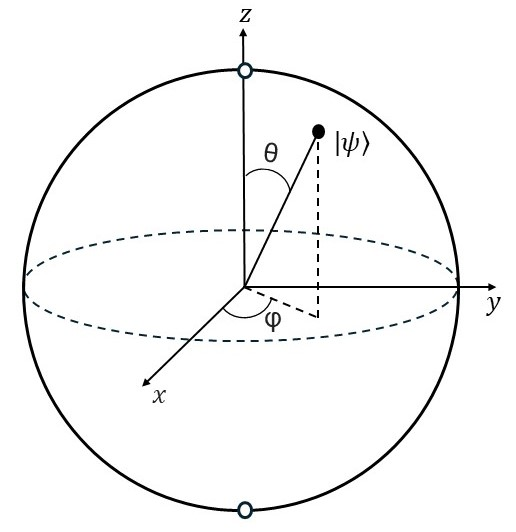
\includegraphics[width=0.35\textwidth]{images/bloch_sphere.jpg}
  \caption{Bloch sphere representation of a qubit}
  \label{fig:bloch_sphere}
\end{figure}

The (trace) distance between two quantum states $\ket{\psi}$ and $\ket{\psi'}$, $\tracenorm{\ket{\psi}-\ket{\psi'}}$, is their Euclidean distance in the Bloch sphere \cite{nielsen2010quantum}. 

There are infinite points in the Bloch sphere, which might suggest the possibility of encoding an infinite amount of information in the infinite binary expansion of the angle $\theta$. However, when a qubit is measured, it collapses to one of the basis states, so only one bit of information can be extracted from a qubit. To accurately determine the amplitudes $\alpha$ and $\beta$, an infinite number of identical qubit copies would need to be measured. Nevertheless, it is still conceptually valid to think of these amplitudes as ``hidden information''. One could say that quantum computation is the art of manipulating this hidden information using phenomena such as interference and superposition to perform tasks that would be impossible or inefficient with classical computers.


% Nota sobre parte final do chuang: informação codificada num qubit e o que perdemos qd medimos um qubit
% Computação quantica é a arte de manipular a informação escondida nos estados quanticos (fenomenos como interferencia e superposição) para realizar tarefas que seriam impossiveis ou ineficientes com computadores clássicos.

\subsection{Multi-qubit States} \label{subsec:entanglement}

\begin{definition}
 The state space of a composite physical system is the \emph{tensor product} of the state spaces of the component physical systems. As a result, an $n$\emph{-qubit state} can be represented by a unit vector in $2^n$-dimensional Hilbert space, $\mathbb{C}^{2^{n}}$. The notations \gls{states-otimes}, \gls{states-no-otimes}, and \gls{states-2gether} are  used to denote the tensor product of two states $\ket{\psi}$ and $\ket{\phi}$. As for any complex vector, $\ket{\psi}^{\otimes n}$ denotes the n-fold tensor product of state $\ket{\psi}$ with itself. The computational basis states of an $n$-qubit system are of the form $\ket{x_{1}\ldots x_{n}}$ and so a quantum state of such a system is specified by $2^{n}$ amplitudes. For instance, a two-qubit state can be written as
\begin{equation*}
  \ket{\psi} = \alpha_{00}\ket{00} + \alpha_{01}\ket{01} + \alpha_{10}\ket{10} + \alpha_{11}\ket{11}.
\end{equation*}
\end{definition}
It should be noted that unfortunately, no simple generalization of the Bloch sphere is known for multiple qubits.

%falta n-fold
%ir ao tensor e acrecentar os operadores que mapeiam operadores

\subsubsection{Entanglement}

\begin{definition}
  An interesting aspect of multi-qubit states is the phenomenon of \emph{entanglement}. This term indicates strong intrinsic correlations between two (or more) particles when the quantum state of each of them cannot be described independently of the state of the other (\ie, it cannot be written as a product of states of the individual qubits). Measuring one qubit of the entangled pair affects the state of the other qubit. This must happen even if the particles are far apart.
\end{definition}

In order to better understand this concept, consider the follow \emph{Bell state} or \emph{EPR pair}:
\begin{equation*}
  \ket{\Phi^{+}} = \frac{1}{\sqrt{2}}(\ket{00} + \ket{11}).
\end{equation*}

Upon measuring the first qubit, there are two possible outcomes: $0$ with probability $1/2$ and $1$ with probability $1/2$. Remarkably, if the first qubit is measured to be $0$, the second qubit will also be $0$ with probability 1; and if the first qubit is measured to be $1$, the second qubit will also be $1$ with probability 1. Therefore, the measurement outcomes are correlated.

These correlations prompted Einstein, Podolsky, and Rosen to publish a paper \cite{einstein1935can} questioning the completeness of quantum mechanics in 1935. The EPR paradox presented a dilemma: the existence of entanglement (\text{i.e.}, correlations that persist regardless of distance) versus local realism and hidden variables. Einstein argued that if two objects, which have interacted in the past but are now separated, exhibit perfect correlation, they must possess a set of properties determined before their separation. These properties would persist in each object, dictating the outcomes of measurements on both sides. Einstein believed that the strong correlations predicted by quantum mechanics necessitate the existence of additional properties not accounted for by the quantum formalism that determine the measurement results. Therefore, he argued that quantum mechanics might require supplementation, as it may not represent a complete or ultimate description of reality.


In 1964, John Bell made a remarkable discovery: the measurement correlations in the Bell state are stronger than those that could ever occur between  classical systems \cite{bell1964einstein}. He explored the idea that each entangled particle might possess hidden properties — unaccounted for by quantum mechanics—that determine the measurement outcomes. Then, through mathematical reasoning, Bell demonstrated that the correlations predicted by any local hidden variable theory cannot exceed a specific level.  There is an upper limit of correlations fixed by what today is called the ``Bell inequalities". He found that quantum theory sometimes predicts correlations that exceed this limit. Consequently, an experiment could  settle the debate by testing whether or not correlations surpass the bounds he had found following Einstein's position.


In 1982, Alain Aspect conducted an experiment that confirmed the violation of the Bell inequalities \cite{aspect1982experimental}. In this experiment, polarizers were placed more than twelve meters apart. This meant that the correlation obtained could not be explained by the fact that the particles carry within them unmeasured properties. Moreover, it proved that the outcome of the measurement is not determined until the moment of measurement. There seemed to be an instantaneous exchange between two particles at the time of measurement when they were twelve meters apart.



Sixteen years later, Nicolas Gisin \cite{tittel1998experimental} and Anton Zeilinger \cite{pan1998experimental} conducted similar experiments, demonstrating that entanglement persists over distances of several kilometers. More recently,  \cite{yin2017satellite} extended these tests using entangled photon pairs sent from a satellite to verify Bell's inequalities over a distance of one thousand kilometers, further confirming that, regardless of the distance, entangled particles behave as an indivisible, inseparable whole. The connection between them is so profound that it appears to challenge the principles of relativity. This phenomenon is known as \emph{quantum nonlocality}.

\subsection{Unitary operators}\label{subsec:unitary-operators}




\subsubsection{Pauli Matrices}
\begin{definition}
The Pauli matrices are a set of three $2 \times 2$ hermitian matrices that are defined as follows:
\begin{equation*}
  \sigma_{x} = \begin{pmatrix} 0 & 1\\ 1 & 0 \end{pmatrix}, \hspace{1cm} \sigma_{y} = \begin{pmatrix} 0 & -i\\ i & 0 \end{pmatrix}, \hspace{1cm} \sigma_{z} = \begin{pmatrix} 1 & 0\\ 0 & -1 \end{pmatrix}.
\end{equation*}
\end{definition}

The eigenvectors and eigenvalues of the Pauli matrices are as follows:
\begin{align*}
 & \sigma_{x} \begin{pmatrix} 1 \\ 1 \end{pmatrix} = \begin{pmatrix} 1 \\ 1 \end{pmatrix}, \hspace{1.4cm} \sigma_{y} \begin{pmatrix} 1 \\ i \end{pmatrix} =  \begin{pmatrix} 1 \\ i \end{pmatrix}, \hspace{1.4cm} \sigma_{z} \begin{pmatrix} 1 \\ 0 \end{pmatrix} = \begin{pmatrix} 1 \\ 0 \end{pmatrix} \\
  & \sigma_{x} \begin{pmatrix} 1 \\ -1 \end{pmatrix} = -\begin{pmatrix} 1 \\ -1 \end{pmatrix}, \hspace{0.7cm} \sigma_{y} \begin{pmatrix} 1 \\ -i \end{pmatrix} = -\begin{pmatrix} 1 \\ -i \end{pmatrix}, \hspace{0.7cm} \sigma_{z} \begin{pmatrix} 0 \\ 1 \end{pmatrix} = -\begin{pmatrix} 0 \\ 1 \end{pmatrix}.
\end{align*}

The normalized eigenvectors of $\sigma_x$ are $\ket{+} = \frac{1}{\sqrt{2}}(\ket{0} + \ket{1})$ and $\ket{-} = \frac{1}{\sqrt{2}}(\ket{0} - \ket{1})$, and normalized eigenvectors of $\sigma_y$ are $\ket{+i} = \frac{1}{\sqrt{2}}(\ket{0} + i\ket{1})$ and $\ket{-i} = \frac{1}{\sqrt{2}}(\ket{0} - i\ket{1})$. The eigenvectors of $\sigma_z$ are $\ket{0}$ and $\ket{1}$. These eigenvectors correspond to the $\hat{x}, \hat{y}$ and $\hat{z}$ axes of the Bloch sphere in \autoref{fig:bloch_sphere}, respectively.

When matrices $\sigma_x, \sigma_y$ or  $\sigma_z$ are applied to a state on the Bloch sphere, they rotate the state by $\pi$ radians around the $\hat{x}, \hat{y}$ or $\hat{z}$ axis, respectively. For example, the action of $\sigma_x$ on the state $\ket{0}$ is to rotate it to $\ket{1}$, and vice versa. Note that for the eigenstates of these matrices with eigenvalue $-1$, this still applies if considering a global phase of $-1 = e^{i\pi}$, given that two quantum states $\ket{\psi}$ and $e^{i\phi}\ket{\psi}$ are indistinguishable by any quantum measurement.

Matrices $\sigma_x$ and $\sigma_z$ will also be referred to as \gls{x} and \gls{z}, respectively.

\subsubsection{Unitary operators}
\begin{definition}
  \emph{Closed systems}, \text{i.e.}, systems that do not interact with other systems evolve according to unitary operators. In quantum computation, these unitary operators are also known as \emph{gates}. For a  state $\ket{\psi}$, a \emph{unitary operator} $U$ describes an evolution from $\ket{\psi}$ to $ U\ket{\psi}$.
\end{definition}

\begin{example}
Pauli matrices are examples of unitary operators. The $X$ and $Z$ gates are often referred to as the \emph{not} and \emph{phase flip} gates, respectively. Other important unitary operators include   \emph{Hadamard gate}, denoted \gls{h}, which maps $\ket{0}$ to $\ket{+}$ and $\ket{1}$ to  $\ket{-}$, and the \emph{phase-shift gate}, denoted $P$, which leaves $\ket{0}$ unaltered applies a phase shift of $\theta$ to the state $\ket{1}$:
\begin{equation*}
 H = \frac{1}{\sqrt{2}}\begin{pmatrix} 1 & 1\\ 1 & -1 \end{pmatrix}, \hspace{1cm} P = \begin{pmatrix} 1 & 0\\ 0 & e^{i \theta} \end{pmatrix}.
\end{equation*}
 
When the Pauli matrices are exponentiated, they result in three valuable classes of unitary matrices, corresponding to the rotation operators around the $\hat{x}$, $\hat{y}$, and $\hat{z}$ axes, which are defined as follows:
\begin{equation*}
  R_{x}(\theta) = e^{-i\theta \sigma_{x}/2} = \text{cos} \left(\frac{\theta}{2} \right) \id -i \text{sin} \left(\frac{\theta}{2} \right) \sigma_{x} = \begin{pmatrix} \cos(\frac{\theta}{2}) & -i\sin(\frac{\theta}{2})\\ -i\sin(\frac{\theta}{2}) & \cos(\frac{\theta}{2}) \end{pmatrix},
\end{equation*}
\begin{equation*}
  R_{y}(\theta) = e^{-i\theta \sigma_{y}/2} = \text{cos} \left(\frac{\theta}{2} \right) \id -i \text{sin} \left(\frac{\theta}{2} \right) \sigma_{y} = \begin{pmatrix} \cos(\frac{\theta}{2}) & -\sin(\frac{\theta}{2})\\ \sin(\frac{\theta}{2}) & \cos(\frac{\theta}{2}) \end{pmatrix},
\end{equation*}
\begin{equation*}
  R_{z}(\theta) = e^{-i\theta \sigma_{z}/2} = \text{cos} \left(\frac{\theta}{2} \right) \id -i \text{sin} \left(\frac{\theta}{2} \right) \sigma_{z} = \begin{pmatrix} e^{-i\theta/2} & 0\\ 0 & e^{i\theta/2} \end{pmatrix}.
\end{equation*}
\end{example}

\begin{theorem} \label{unitary} \cite{nielsen2010quantum}
  Suppose $U$ is a unitary operation on a single qubit. Then there exist real numbers $\alpha$, $\beta$, $\gamma$ and $\delta$ such that
  \begin{equation*}
    U = e^{i\alpha} R_{z}(\beta) R_{y}(\gamma) R_{z}(\delta).
  \end{equation*}
\end{theorem}

\begin{example}
  
There are also multi-qubit gates, such as the \emph{controlled-not} gate, denoted \gls{cnot}, in which the state of the first qubit determines whether the \( X \) gate is applied to the second qubit. The first qubit is called the \emph{control qubit}, and the second is the \emph{target qubit}. The gate is defined by the following matrix:
\begin{equation*}
  \textit{CNOT} = \begin{pmatrix}
    1 & 0 & 0 & 0 \\
    0 & 1 & 0 & 0 \\
    0 & 0 & 0 & 1 \\
    0 & 0 & 1 & 0
  \end{pmatrix}.
\end{equation*}
In this case, the states \( \ket{00} \) and \( \ket{01} \) remain unchanged, while \( \ket{10} \) and \( \ket{11} \) are mapped to each other.

There is an ``extension" of the controlled-not gate, the controlled-$U$ gate, where $U$ is a unitary gate acting on a single qubit. This gate applies the gate $U$ to the target qubit if the control qubit is in state $\ket{1}$ and does nothing otherwise. It is defined as:
\begin{align*}
  &\textit{CU} (\ket{0} \otimes \ket{\psi}) = \ket{0} \otimes \ket{\psi}\\ 
  &\textit{CU} (\ket{1} \otimes \ket{\psi}) = \ket{1} \otimes U\ket{\psi}.
\end{align*}
\end{example}

It should be noted that no completely closed systems exist in the universe. Nevertheless, for many systems, the approximation of a closed system is valid.
% No fim nota sobre não haver sistemas completamente fechados no universo, mas que a aproximação de um sistema fechado é válida para muitos sistemas, p.82



\subsection{Measurements} \label{subsec:Measurements}

% decidir se e como por M0 e M1

There are times when it necessary to observe the system to extract information. This interection leaves the system no longer closed and, consequently, the evolution of the system is no longer unitary. 

\begin{definition}
The act of measuring a qubit is represented by a set of operators called \emph{measurement operators}, denoted $\{M_{m}\}$. These operators act on the state space  of the system being measured. The index $m$ refers possible measurement outcomes. These measurement operators must satisfy the completeness equation $\sum_{m} M_{m}^{\dagger}M_{m} = \id$, which ensures that the probabilities of all possible outcomes sum to 1. If a measurement ${M_m}$ is performed on a state $\ket{\psi}$ the outcome $m$ is observed with probability $p_m = \bra{\psi}M_{m}^{\dagger}M_{m}\ket{\psi}$ for each $m$. Moreover, after a measurement yielding outcome $m$, the state collapses to 
\begin{align*}
  \ket{\psi'}=\frac{M_{m}\ket{\psi}}{\sqrt{p_{m}}}.
\end{align*}
\end{definition}

\begin{definition}
  A measurement is called a \emph{projective measurement} if its measurement operators are projectors.
\end{definition}

\begin{example}
In the case of the computational basis, the measurement operators are the projectors onto the basis states $\ket{0}$ and $\ket{1}$ denoted by $M_{0} = \ket{0}\bra{0}$ and $M_{1} = \ket{1}\bra{1}$, respectively. Considering an arbitrary state $\ket{\psi} = \alpha \ket{0} + \beta \ket{1}$, the probabilities of measuring 0 and 1 are $p_0 = \bra{\psi} M_{0} M_{0}^{\dag}\ket{\psi}=\bra{\psi} M_{0} \ket{\psi} = |\alpha|^{2}$, and $p_1 = \bra{\psi} M_{1} M_{1}^{\dag}\ket{\psi} = \bra{\psi} M_{1} \ket{\psi} =  |\beta|^{2} $, respectively. Consequently the states after measurement are
\begin{align*}
  &\ket{\psi'}=\frac{M_{0}\ket{\psi}} {|\alpha|} = \frac{\alpha}{|\alpha|} \ket{0} = \ket{0} (\text{with  } p=p_0) \quad \text{and } \\
  &\ket{\psi''}= \frac{M_{1}\ket{\psi}} {|\beta|} = \frac{\beta}{|\beta|} \ket{1} = \ket{1} (\text{with  } p=p_1)
\end{align*}
\end{example}


From now on, unless stated otherwise, any reference to measurement should be understood as pertaining to the computational basis.

As previously mentioned, any states $\ket{\psi}$ and $e^{i\phi}\ket{\psi}$ are indistinguishable by any quantum measurement. Consider a measurement operator $M_m$, the probabilities of obtaining outcome $m$ are $\bra{\psi} M_{m}^{\dagger}M_{m}\ket{\psi}$ and $\bra{\psi} e^{-i \theta} M_{m}^{\dagger}M_{m}e^{i\theta}\ket{\psi}=\bra{\psi} M_{m}^{\dagger}M_{m}\ket{\psi}$. For this reason, it is said that these states are equal from an observational point of view.



%If a measurement ${M_m}$ is performed on a state $\rho$, the outcome $m$ is observed with probability $p_m = \text{Tr}(M_{m} \rho M^{\dag}_{m})$ for each $m$. Moreover, after a measurement yielding outcome $m$, the state collapses to $M_{m}\rho M^{\dag}_{m}/p_{m}$. 
% ver p.93

\subsection{Density operators}
Until now the state vector formalism was used. However there is an alternative formulation using density operators. The density operator is often known as the \emph{density matrix}, the two terms will be used interchangeably.

%\subsubsection{General properties}

\begin{definition}
A quantum state $\ket{\psi}$ is said to be a \emph{pure state} if it is completely known, \ie if it can be written as a ket. In this case, the state can be written in the density operator formalism as $\rho = \ket{\psi}\bra{\psi}$. 
\end{definition}

\begin{definition}
A state that is a probabilistic mixture of pure states is designated a \emph{mixed state}. A mixed state can be represented by a density operator $\rho= \sum_i |p_i|^{2}\ket{\psi_i}\bra{\psi_i}$, where $|p_i|^{2}$ is the probability of the system being in state $\ket{\psi_i}$.
\end{definition} 

\begin{definition}[Unitary Evolution of a Density Operator]
  When a unitary operator \( U \) is applied to a mixed quantum state described by a density matrix \( \rho \), the resulting state is given by $ \rho' = U \rho U^\dagger.$
\end{definition}

\begin{definition}[Measurement of a Density Operator]
  Given a collection of measurement operators \( \{M_m\} \), the probability of obtaining outcome \( m \) when measuring a state \( \rho \) is $p_m = \text{Tr}(M_m \rho M_m^\dagger).$
  After observing outcome $ m $, the post-measurement state collapses to:
  \[
  \rho' = \frac{M_m \rho M_m^\dagger}{\text{Tr}(M_m \rho M_m^\dagger)}.
  \]
\end{definition}


\begin{definition}
  In \autoref{subsec:hilb2D} it was shown how to determine the cartesian coordenates of a pure state in the Bloch sphere from the state vector. For an arbitrary $2 \times 2$ density matrix, the following holds
\begin{equation} \label{eq:bloch_vector_0}
  \rho = \frac{1}{2}(\id + r_{x}\sigma_{x} + r_{y}\sigma_{y} + r_{z}\sigma_{z}),
\end{equation}
where $r = (r_x, r_y, r_z)$ is a real three-dimensional vector such that $\| r \|_2 \leq 1$. This vector is known as the \emph{Bloch vector for the state} $\rho$. Since $\rho$ is Hermitian, $r_x, r_y$ and $r_z$ are always real.  

To derive the inverse map \( r_\mu = \text{Tr}(\rho \sigma_\mu) \), consider the properties of Pauli matrices:
\[
\text{Tr}(\sigma_\mu) = 0, \quad \text{Tr}(\sigma_\mu \sigma_\nu) = 2 \delta_{\mu \nu}.
\]

Consequently,
\[
\text{Tr}(\rho \sigma_\mu) = \frac{1}{2} \sum_{\nu} r_\nu \text{Tr}(\sigma_\nu \sigma_\mu) = \frac{1}{2} \cdot 2 r_\mu = r_\mu.
\]

Thus, the inverse map of \autoref{eq:bloch_vector_0} is
\begin{equation}
  \label{eq:Bloch_vector}
  r_{\mu} = \text{Tr}(\rho \sigma_{\mu}).
  \end{equation} 
\end{definition}


  Note that given that the trace is linear and matrix multiplication distributes over matrix addition, the cartesian coordinates of an operator consisting of the sum or subtraction of density operators can also be determined by \autoref{eq:Bloch_vector}.

\subsubsection{Reduced density operator}

Density operators are particularly well-suited for describing individual subsystems of a composite quantum system. This type of description is provided by the \emph{reduced density operator}

\begin{definition}
Consider Hilbert spaces $\mathcal{H}_A$ and $\mathcal{H}_B$ of systems $A$ and $B$, respectively. The \emph{partial trace over $B$},$\tr_B \colon \mathcal{T}(\mathcal{H}_A \otimes \mathcal{H}_B) \to \mathcal{T}(\mathcal{H}_A)$,
is defined by
\[
\tr_B = \text{id}_{\mathcal{T}(\mathcal{H}_A)} \otimes \tr.
\]
Similarly, the \emph{partial trace over $B$} corresponds to the map \(
\tr_A \colon \mathcal{T}(\mathcal{H}_A \otimes \mathcal{H}_B) \to \mathcal{T}(\mathcal{H}_B),
\)
defined by 
\[
\tr_B = \tr \otimes \text{id}_{\mathcal{T}(\mathcal{H}_B)}.
\]
\end{definition}

\begin{comment}
\begin{align*}
  \text{Tr}_{B}(\ket{a_1}\bra{a_2} \otimes \ket{b_1}\bra{b_2}) & =\ket{a_1}\bra{a_2}\text{Tr}(\ket{b_1}\bra{b_2}) \\
  & = \ket{a_1}\bra{a_2}  \sum_{\mu} \bra{\mu} \ket{b_1}\bra{b_2} \ket{\mu} \\
  & =  \ket{a_1} \bra{a_2} \sum_{\mu} \braket{\mu} {b_1}\braket{b_2} {\mu} \\
  & = \ket{a_1} \bra{a_2} \sum_{\mu} \braket{b_2}{\mu} \braket{\mu}{b_1} \\
  &= \ket{a_1}\bra{a_2}  \braket{b_2}{b_1}
\end{align*}
where \( \{\ket{\mu}\} \) is an orthonormal basis spanning the state space of \( B \).
In certain situations it is more advantageous to consider the reduced density operator for subsystem $A$ defined as:
\begin{equation*}
  \rho_{A} = \text{Tr}_{B}(\rho_{AB}) = \sum_{\mu} \bra{\mu} \rho_{AB} \ket{\mu},
\end{equation*}
where $\{\ket{\mu}\}$, span the state space of $B$ and act only in the state space of $B$. 
\end{definition}
\end{comment}

\begin{definition}
Given physical systems $A$ and $B$ whose composite system is given by the density operator $\rho_{AB}$, the \emph{reduced density operator} for subsystem $A$ is $\rho_{A} = \text{Tr}_{B}(\rho_{AB}).$
Similarly, the \emph{reduced density operator for subsystem} $B$ is $\rho_{B} = \text{Tr}_{A}(\rho_{AB})$.
\end{definition}

Recall that in this section we restrict ourselves to the finite-dimensional setting, where the set of trace class operators on $\HilbH$, $\TraceOp{\HilbH}$, can be identified with the set of bounded operators on $\HilbH$, $\BoundOp{\HilbH}$.
Nevertheless, we use the notation $\TraceOp{\HilbH}$, as it reflects the natural setting of the density operator formalism --- a density operator must be trace-class, even in the infinite-dimensional case \cite{heinosaariMathematicalLanguageQuantum2011}.


%to emphasize that a density operator must be trace-class (the infinite-dimensional extension of the definition of density operator(\autoref{def:density_op}) requires it to be trace-class). 

 %\begin{align*}
 %\text{Tr}_{B}(\ket{a}\bra{b} \otimes \ket{c}\bra{d}) & =\ket{i}\bra{j} \text{Tr}(\ket{k}\bra{l}) \\
 %&= \ket{a}\bra{b} \sum_{\mu} \bra{\mu} \ket{c}\bra{d}  \ket{\mu} \\
 %& = \sum_{\mu} \bra{\mu} \ket{a} \bra{b} \otimes \ket{c} \bra{d} \ket{\mu} 
%\end{align*}
%where $\ket{a}$ and $\ket{b}$ are any two vectors in the state space of $A$,  $\ket{c}$ and $\ket{d}$ are any two vectors in the state space of $B$, and $\{\ket{\mu}\}$, span the state space of $B$, act only in the state space of $B$. Therefore, by linearly, the partial trace of $\rho_{AB} = \sum_{ij} p_{ij} \ket{a_i} \bra{b_i}  \otimes \ket{c_j} \bra{d_j}  $ is




%An $n$-qubit mixed state can be represented by a density operator $ \mathbb{C}^{2^{n}} \xrightarrow{} \mathbb{C}^{2^{n}}$, whose matrix representation is $\rho = \Sigma_{i} \hspace{2pt} p_{i} \vert \phi_{i} \rangle \langle \phi_{i} \vert$. A density operator encodes uncertainty about the current state of the quantum system at hand. For example, a mixed state with half probability of $\vert 0 \rangle$ and $\vert 1 \rangle$ can be represented by $\frac{\vert 0 \rangle \langle 0 \vert + \vert 1 \rangle \langle 1 \vert}{2}=I/2$, where $I$ is the identity matrix.  One usually denotes density matrices by the greek letters $\rho$, $\sigma$, and so forth. The set of density operators is denoted by $\mathcal{D}_{n} \subseteq \mathbb{C}^{ 2^{n \times n}}$.

% tudo sobre matrizes de densidade incuindo a definição de matriz de densidade reduzida e traço parcial

% bloch vector for mixed states



\subsection{Quantum Channels} \label{subsec:quantum_channels}

% Fazer secção chamada quantum chanels e falar de super operadores e cptp maps, normas, kraus operators

Thus far, only two types of quantum operations have been discussed: unitary operators, which describe the evolution of a closed quantum system, and measurements, which describe the act of observing a quantum system. Now, a new type of quantum operation that accounts for the more realistic notion of interaction between a quantum system and an environment will be introduced. Nonetheless, it is necessary to first introduce a few key concepts. 


\vspace{5pt}
%the evolution of a quantum system has been described by unitary operators. However, in practice, quantum systems are not isolated, and they interact with their environment. This interaction is described by a \emph{quantum channel}, which is a completely positive trace-preserving (CPTP) linear map. A quantum channel is a generalization of a unitary operator that allows for the description of the evolution of a quantum system under the influence of an environment.

In this perspective, we focus on quantum states, represented by density operators. Consequently, we are also interested in \emph{state transformers}---operators that map density operators to density operators.

\begin{definition}
 Operators that map operators to other operators are known as \emph{super-operators}. 
\end{definition}


\begin{definition} \label{def:positive_superoperator}
  A super-operator $\Phi: \TraceOp{\HilbH} \to \TraceOp{\HilbK} $ is called \emph{positive} if it sends positive operators to positive operators, \textit{i.e.} $A \geq 0 \Rightarrow{} Q A \geq 0$.
\end{definition}

\begin{definition}
  The tensor product of two super-operators 
  $\Phi: \TraceOp{\HilbH_1} \rightarrow \TraceOp{\HilbK_1} $ 
  and
  $\Psi : \TraceOp{\HilbH_2} \rightarrow \TraceOp{\HilbK_2}$ 
  is an operator 
  $ \Phi \otimes \Psi:  \TraceOp{\HilbH_1 \otimes \HilbK_1} \rightarrow \TraceOp{\HilbH_2 \otimes \HilbK_2}$ 
  defined by the equation:
\begin{equation*}
  (\Phi \otimes \Psi)(A \otimes B) = \Phi (A) \otimes \Psi(B).
\end{equation*}
\end{definition}

\begin{definition} \label{def:completely_positive_superoperator}
  A linear mapping $ \Phi : \mathcal{T}(\HilbH_1) \to \mathcal{T}(\HilbH_2)$ is \emph{completely positive} if the mapping 
$\Phi \otimes \id_{\mathcal{T}(\HilbK)}$ on $\mathcal{T}(\mathcal{H}_1 \otimes \HilbK) \to \mathcal{T}(\HilbH_2 \otimes \HilbK) $ is positive for any Hilbert space $\HilbK$.
\end{definition}

\begin{definition} \label{def:trace_preserving_superoperator}
  A super-operator $\Phi$ is called \emph{trace-preserving} (resp. \emph{trace-nonincreasing}) if $\text{Tr} \hspace{2pt} (\Phi A)= \text{Tr} (A) $ (resp. ($\text{Tr} \hspace{2pt} (\Phi A)\leq \text{Tr} (A)$)).
\end{definition}

Since density matrices are positive, any physically allowed transformation must be represented by a positive operator. Nonetheless, this is not sufficient on its own: since one can always extend the space $\mathbb{C}^{n \times n}$ to  $\mathbb{C}^{n \times n} \otimes \mathbb{C}^{m \times m} $ by adjoining a new quantum system, any physically allowed transformation must be completely positive. Finally, since the trace of a density matrix is always $1$, any physically allowed transformation must be trace-preserving. A \acrfull{cptp} operator is traditionally called a \emph{quantum channel}.


It is sometimes convenient to relax the trace-preserving condition to a trace-non-increasing condition, resulting in what is known as a \emph{quantum operation}. This accounts for phenomena such as \emph{qubit leakage} (the unintended loss of quantum information from computational basis states, $\ket{0}$ and $\ket{1}$, into higher-energy non-computational states, e.g., $\ket{2}$, $\ket{3}$, breaking the idealized two-level qubit assumption) and operations such as \emph{postselection} (a technique in quantum algorithms where operations are conditioned on measurement outcomes, often leading to non-trace-preserving maps) \cite{Yu_trace_non_inc}.









\subsubsection{Kraus operator sum representation}


Assume that there is a quantum system $S$ of interest which is a subsystem of a larger system which also includes an environment $E$. These systems have a joint unitary evolution described by a unitary operator $U$ acting on the composite system, $U (\rho_{SE} )= U \rho_{SE} U^{\dag}$. 

Given that density matrices are positve operators, and therefore Hermitian with non-negative eigenvalues, the density operator of the environment $\rho_E$ initially can be written as 
\begin{equation*}
  \rho_E = \sum_{i} p_{i} \ket{i} \bra{i}
\end{equation*}
where $\ket{i}$ form an orthonormal basis for the state space of $E$ and $p_{i}$ are positive. 

The state of the subsystem $S$ after the unitary evolution corresponds to the partial trace of the joint state over the environment,
\begin{align*}
  \rho_{S}' = & \text{Tr}_{E}(U \rho_{SE} U^{\dag}) \\
 = & \sum_{\mu} \bra{\mu} U \rho_{SE} U^{\dag} \ket{\mu}
\end{align*}
where $\{\ket{\mu}\}$ span the state space of $E$.

 
Considering that initially both systems are completely decoupled, the initial state of the system can be written as $ \rho_{SE} = \rho_{S} \otimes \rho_{E}$. Thus,
\begin{align*} 
  \rho_{S}' = & \sum_{\mu} \bra{\mu} U \rho_{S} \otimes \sum_{i} p_{i} \ket{i} \bra{i} U^{\dag} \ket{\mu} \\
  = & \sum_{\mu i}  \sqrt{p_{i}} \bra{\mu} U \ket{i} \rho_{S} \sqrt{p_{i}} \bra{i} U^{\dag} \ket{\mu}  \\ 
  = & \sum_{\mu i} \text{K}_{\mu i} \rho_{S} \text{K}_{\mu i}^{\dag}
\end{align*}
where the set of operators $\{\text{K}_{\mu i}\}$ is designated \emph{Kraus operators} and $\text{K}_{\mu i} = \sqrt{p_{i}} \bra{\mu} U \ket{i}$. Note that $\{\ket{\mu}\}$ and $\{\ket{i}\}$, act only in the state space of $E$. 

\begin{definition}
  The equation $ \rho_{S}' = \sum_{\mu i} \text{K}_{\mu i} \rho_{S} \text{K}_{\mu i}^{\dag} $ is called an \emph{\acrfull{osr}}. An OSR can be thought of as a quantum channel that maps $\rho_{S}$ to $\sum_{\mu i} \text{K}_{\mu i} \rho_{S} \text{K}_{\mu i}^{\dag}$, given this map is CPTP \cite{lidar2019lecture, watrous2018theory}. 
\end{definition}




\subsubsection{Non-selective measurements}

In the previously presented formalism to represent all the possible outcomes of a measurement, described by a set of operators $\{M_{m}\}$, on a state $\rho$, it would be necessary to write that state $\rho$ collapse to state $\rho_m=\frac{M_{m}^{\dag}\rho M_{m}}{\text{Tr}(M_{m}\rho M_{m}^{\dag})}$ with probability $p_m=\text{Tr}(M_{m}\rho M_{m}^{\dag})$, for each possible outcome $m$. Although the selective description above is useful conceptually, it is often impractical for calculations. Instead, one uses \emph{non-selective measurements}, in which the possible outcomes are not explicitly stated.


\begin{definition}
A \emph{non-selective measurement} is a quantum measurement in which the post-measurement state of the system is then given by the weighted sum over all possible outcomes:
\[
\rho = \sum_m p(m) \rho_m = \sum_m M_m \rho M_m^{\dag}.
\]
This last equality corresponds to an Kraus operator sum representation, where the set of Kraus operators is $\{M_{m}\}$.
\end{definition}

\subsection{Norms on quantum channels}
\begin{definition} \label{def:trace_norm_superoperator}
  The trace norm of a super-operator $\Phi: \TraceOp{\HilbH} \rightarrow \TraceOp{\HilbK}$ is defined as:
  \begin{equation*} 
    \lVert \Phi \rVert_{1} =  \sup\{\lVert \Phi \hspace{1pt} A \rVert_{1}   \mid  \lVert A \rVert_{1}=1\}, 
  \end{equation*}
\end{definition}
where $A \in \TraceOp{\HilbH}$.

%\begin{theorem} \label{thm:Russo–Dye} \cite[Theorem 3.39]{watrous2018theory}
  %Let $Q: \mathbb{C}^{n \times n} \rightarrow \mathbb{C}^{m \times m}$ be a positive super-operator and $u \in \mathbb{C}^{n}$. It holds that 
  %\begin{equation}
    %\lVert Q \rVert_{1} = \max \{\text{Tr}\left(Q(uu^{*}) \right) \vert \hspace{2pt}  \lVert u \rVert_{1}=1 \}.
  %\end{equation}
%\end{theorem}

%\begin{proposition} \cite[Proposition 3.41]{watrous2018theory}
%The following facts hold for the trace norm:
%\begin{enumerate}
  %\item The trace norm is submultiplicative with respect to composition of super-operators , \textit{i.e.}, for all super-operators  $Q: \mathbb{C}^{n \times n} \rightarrow \mathbb{C}^{m \times m}$ and $S: \mathbb{C}^{m \times m} \rightarrow \mathbb{C}^{o \times o}$
  %\begin{equation}
    %\lVert S  Q \rVert_{1} \leq \lVert S \rVert_{1} \lVert Q \rVert_{1}.
  %\end{equation}
  %\item Let $U_0,$ $V_0 \in \mathbb{C}^{n\times n}$ and $U_1,$ $V_1 \in \mathbb{C}^{m\times m}$ be unitary operators, let $Q,$ $S: \mathbb{C}^{n \times n} \rightarrow \mathbb{C}^{m \times m}$ be super-operators, where $S$ is defined as:
  %\begin{equation}
    %S(X) = U_1 Q(U_0 A V_0) V_1
 % \end{equation}
  %for all $A \in \mathbb{C}^{n\times n}$. It holds that $\lVert Q \rVert_{1} = \lVert S \rVert_{1} $.
%\end{enumerate}
%\end{proposition}


Unfortunately, this norm is not stable under tensoring , given that the inequation $ \lVert \Phi \otimes I_{\TraceOp{\HilbH}} \rVert_{1} \geq \lVert \Phi \rVert_{1}$ does not hold \cite{watrous2018theory}. As a result, the diamond norm, which is based on the trace norm, is used instead in the context of quantum channels. 

\begin{definition} \label{def:diamond_norm}
  Given a super-operator $\Phi: \TraceOp{\HilbH} \to \TraceOp{\HilbK}$, the diamond norm, \gls{diamond-norm}, is defined as:
  \begin{equation*}  \label{eq:diamond_distance}
    \lVert \Phi \rVert_{\diamondsuit} =  \lVert \Phi \otimes \id_{\TraceOp{\HilbH}} \rVert_{1}
  \end{equation*}
\end{definition}


%For this norm it holds that for all super-operators $Q: \mathbb{C}^{n \times n}\rightarrow \mathbb{C}^{m \times m} $ and $S:\mathbb{C}^{m \times m} \rightarrow \mathbb{C}^{o \times o} $, if $Q$ is a quantum channel then $\lVert S  Q \rVert_{\diamondsuit} \leq \lVert S \rVert_{\diamondsuit}$ \cite[Proposition 3.44 and Proposition 3.48]{watrous2018theory}, and if $S$ is a quantum channel, then $\lVert S  Q \rVert_{\diamondsuit} \leq \lVert Q \rVert_{\diamondsuit}$. This is a desireble property, as is guarantees that quantum operations do not increase the distance between states, and as a
%consequence, composition of programs is valid.


Since the diamond norm is generally difficult to compute, we will rely on the following properties:


\begin{theorem} \label{thm:russo_dye}
Let \(\Phi \in \mathcal{T}(\HilbH) \to \mathcal{T}(\HilbK)\) be a positive map. Then it holds that
\[
\tracenorm{\Phi}= \sup \{ \operatorname{Tr} \left( \Phi(vv^*) \right) \, \vert \, \euclideannorm{v}=1, v\in \HilbH  \}.
\]
\end{theorem}

\begin{proposition} \cite[Proposition 3.48]{watrous2018theory} \label{prop:diamond_submult}
  For all maps \(\Phi \in \mathcal{T}(\HilbH) \to \mathcal{T}(\HilbK)\) and \(\Psi \in \mathcal{T}(\HilbK) \to \mathcal{T}(\HilbL)\), it holds that
  \begin{align*}
    \diamondnorm{\Psi \Phi} \leq  \diamondnorm{\Psi} \diamondnorm{\Phi}. 
  \end{align*}
\end{proposition}

\begin{theorem} \cite[Theorem 3.49]{watrous2018theory}\label{thm:diamond_tensor_comp}
  Let $\Phi \in \mathcal{T}(\HilbH_1) \to \mathcal{T}(\HilbK_1)$ and \(\Psi \in \mathcal{T}(\HilbH_2) \to \mathcal{T}(\HilbK_2)\) be maps. Then it holds that
\[
\diamondnorm{\Phi \otimes \Psi} = \diamondnorm{\Phi}\diamondnorm{\Phi}
\]
\end{theorem}

\begin{theorem} \cite[Theorem 3.55]{watrous2018theory} \label{theorem:diamond_iso}
  Let  $ n \leq m$, let $V_0,V_1: \TraceOp{\HilbH,\HilbK}$ be isometries, and define CPTP operators $\Phi_0,\Phi_1:\TraceOp{\HilbH} \to \TraceOp{\HilbK}$ as
\[
\Phi_0(\rho) = V_0 \rho V_0^\dag \quad \text{and} \quad \Phi_1(\rho) = V_1 \rho V_1^\dag
\]
for all $\rho \in \TraceOp{\HilbH}$. There exists a unit vector $u \in \HilbH $ such that
\[
\tracenorm{\Phi_0(uu^\dag) - \Phi_1(uu^\dag)} = \diamondnorm{\Phi_0 - \Phi_1}.
\]
\end{theorem}

\begin{theorem} \cite[Theorem 3.56]{watrous2018theory} \label{theorem:diamond_cptp_id}
 Let $\Phi:\TraceOp{\HilbH} \to \TraceOp{\HilbK} $ be a quantum channel, let $\varepsilon \in [0,2]$, and suppose that
    \[
    \|\phi(\rho) - \rho\|_1 \leq \varepsilon
    \]
    for every density operator $\rho \in \TraceOp{\HilbH}$. It holds that
    \[
    \|\phi - \id_{\TraceOp{\HilbH}}\|_1 \leq \sqrt{2\varepsilon}.
    \]
\end{theorem}





\subsection{Quantum circuits}
As quantum computation remains in its early stages of development, programming is primarily based on the use of \emph{quantum circuits}. 

\begin{definition}
  A \emph{quantum circuit} consists of wires and quantum gates, which serve to transmit and manipulate quantum information. Each wire corresponds to a qubit, while the gates represent operations that can be applied to these qubits. 
\end{definition}

In this subsection the notation for the quantum gates used in this work will be introduced.

Wires in parallel represent the tensor product of the respective qubits. For instance, $\psi_0 \otimes \psi_1$ corresponds to
\begin{figure} [H]
  \centering
  \begin{quantikz} [column sep=0.5cm, row sep=0.8cm] 
      \lstick{$\ket{\psi_0}$} & \qw & \qw & \qw \\
      \lstick{$\ket{\psi_1}$} & \qw & \qw & \qw 
 \end{quantikz}
\end{figure}

The single bit gates presented in \Cref{subsec:unitary-operators} are represented as a box with the symboL of the gate inside. For example, the Hadamard gate is represented as
\begin{figure} [H]
  \centering
  \begin{quantikz} [column sep=0.5cm, row sep=0.8cm] 
       & \gate{H} & \qw
 \end{quantikz}
\end{figure}

The controlled-not gate, which is a two-qubit gate, is represented as
\begin{figure} [H]
  \centering
  \begin{quantikz} [column sep=0.5cm, row sep=0.8cm] 
      & \ctrl{1} & \qw \\
       & \targ{} & \qw 
 \end{quantikz}
\end{figure}

Similarly, the controlled-$U$ gate, where $U$ is an unitary single-qubit gate, is represented as
\begin{figure} [H]
  \centering
  \begin{quantikz} [column sep=0.5cm, row sep=0.8cm] 
      & \ctrl{1} & \qw \\
       & \gate{U} & \qw 
 \end{quantikz}
\end{figure}

An arbitrary unitary operator acting on $n$ qubits is represented as a box acting on $n$ wires. For instance, the operator $U$ acting on two qubits is represented as
\begin{figure} [H]
  \centering
  \begin{quantikz} [column sep=0.5cm, row sep=0.8cm] 
      & \gate[wires=2]{U} & \qw \\
      & &\qw
 \end{quantikz}
\end{figure}

CPTP maps are depicted as boxes containing the corresponding map symbols.

The measurement operation is representes by a ``meter'' symbol. Given that output of a measurement is a classical bit, the wire representing the output of a measurement is a classical wire, represented by a double line. 

\begin{figure} [H]
  \centering
  \begin{quantikz} [column sep=0.5cm, row sep=0.8cm] 
      & \meter{} & \setwiretype{c}  
 \end{quantikz}
\end{figure}



\subsection{No-cloning theorem}
The no-cloning theorem states that it is impossible to duplicate an unknown quantum bit \cite{wootters1982single}. In this subsection, an elementary proof of this theorem will be presented.

Suppose that there exists a cloning machine, $C$, that produces a clone (a duplicate) of any unknown state. It recieves a qubit $\ket{\psi}$ and some standard pure state $\ket{s}$ as input and returns the state $\ket{\psi} \otimes \ket{\psi}$.

takes one state as input and returns two of the same kind. The second is a duplicate of the first in the sense that no experiment could distinguish between them. Hence, the action of a clonning machine can be written as
\[
|\psi\rangle \otimes |s\rangle \mapsto |\psi\rangle \otimes |\psi\rangle
\]
for all states $|\psi\rangle$.

However, due to its violation of linearity, this kind of transformation is not a valid quantum operation. Namely, let $|\psi\rangle = \sum_i \alpha_i \ket{\psi_i}$ be a mixed state. Then:
\begin{equation*}
C \left( \sum_i \alpha_i |\psi_i\rangle \right) \otimes |s\rangle 
=
 \left( \sum_i \alpha_i |\psi_i\rangle \right) \otimes  \left( \sum_i \alpha_i |\psi_i\rangle \right)  =  \sum_{i,j} \alpha_i \alpha_j |\psi_i\rangle \otimes |\psi_j\rangle,
\end{equation*}
but assuming linearity of the cloning transformation, we would get:
\begin{equation*}
 C \left( \sum_i \alpha_i |\psi_i\rangle \right)  \otimes |s\rangle =  \sum_i \alpha_i C \left(|\psi_i\rangle \right)
=
\sum_i \alpha_i \left( |\psi_i\rangle \otimes |\psi_i\rangle \right).
\end{equation*}

These two expressions generally do not coincide. For instance, let $\{|\psi_i\rangle\}$ be a set of orthogonal pure states. In this case, the coefficients $\alpha_i \alpha_j $ and $\alpha_i$ correspond exactly to the eigenvalues of the final states in the equations above. Since $ \alpha_i \alpha_j < \alpha_i$ for all $\alpha_j< 1$, the two resulting states are distinct.


\begin{comment}
Suppose that there exists a unitary operator $U$ that recieves a qubit $\ket{\psi}$ and some standard pure state $\ket{s}$ as input and oututs the state $\ket{\psi} \otimes \ket{\psi}$. The action of $U$ can be written as
\begin{equation*}
  U \left(\ket{\psi} \otimes \ket{s} \right) = \ket{\psi} \otimes \ket{\psi}
\end{equation*}
Consider the aplication of $U$ to two pure states $\ket{\psi_0}$ and $\ket{\psi_1}$,
\begin{align*}
  U \left(\ket{\psi_0} \otimes \ket{s} \right) = \ket{\psi_0} \otimes \ket{\psi_0} \\
  U \left(\ket{\psi_1} \otimes \ket{s} \right) = \ket{\psi_1} \otimes \ket{\psi_1}.
\end{align*}

Given that unitary operators preserve inner products, the following equality should hold:
\begin{equation*}
  \braket{\psi_0}{\psi_1} = ( \braket{\psi_0}{\psi_1})^{2}
\end{equation*}

This equation is only satisfied if $\braket{\psi_0}{\psi_1} = 0$ or $\braket{\psi_0}{\psi_1} = 1$. The first case implies that $\ket{\psi_0}$ and $\ket{\psi_1}$ are orthogonal, and the second case implies that they are in the same state. Therefore, it is only possible to clone orthogonal states. These are the states perfectly distinguishable by measurement and thus are equivalent to copying classical information. For instance, it is impossible to the clone qubits $\psi_0 = \ket{0}$ and $\psi_1 = \ket{-}$, since they are not orthogonal.
\end{comment}

It should be noted that this principle is upheld by the type system outlined in \autoref{fig:typing_rules_linear}, which does not allow the repeated use of a variable (seen as a quantum resource).






\section{\( W^* \)-Algebras}

In this section, we are no longer restricted to finite-dimensional vector spaces; the term ``vector space" now also encompasses infinite-dimensional ones. 

\begin{comment}
We would like to focus instead on the
 category of von Neumann algebras and completely positive normal subunital maps, vNACPsU,
 as it seems more appropriate for modelling quantum computation: the full subcategory
 of vNAop
 CPsU consisting of finite dimensional von Neumann algebras is equivalent to Selinger’s
 category Q [35], which is used to model first order quantum programming languages.
\end{comment}


 While quantum theory is traditionally formulated in terms of Hilbert spaces, there is also a more abstract and general formulation using operator algebras. This perspective traces back to Heisenberg’s work on the spectral lines of the hydrogen atom in 1925, where he realized that observable quantities in quantum systems, such as the position of an electron in a hydrogen atom, are better represented by infinite arrays of complex numbers \cite{heisenbergUeberQuantentheoretischeUmdeutung1925}. Born and Jordan subsequently recognized that these arrays should follow the rules of matrix multiplication \cite{bornZurQuantenmechanik1925}. To address the mathematical challenges posed by infinite matrices, Von Neumann formalized these ideas using operators on Hilbert spaces, more concretely, \emph{Von Neumann} algebras \cite{neumann1927wahrscheinlichkeitstheoretischer}. This gave rise to the study of operator algebras, which are now applied in various domains in quantum theory, including quantum statistical mechanics \cite{bratteliOperatorAlgebrasQuantum1987}, quantum field theory \cite{arakiMathematicalTheoryQuantum1999,haagAlgebraicApproachQuantum1964}, and quantum information theory \cite{keylFundamentalsQuantumInformation2002}. We refer to the abstract characterization of von Neumann algebras as $W^*$-algebras, although the terms are often used interchangeably in the literature.


 While $C^*$-algebras can also model quantum computing, $W^*$-algebras may be more suitable for this purpose. For instance, whereas $C^*$-algebras correspond to noncommutative geometry \cite{connesNoncommutativeGeometry1995}, $W^*$-algebras can be viewed as noncommutative analogues of measure theory or probability, aligning with the probabilistic nature of quantum \cite{hamhalterQuantumMeasureTheory2003,HansQuantumProbabilityQuantumInformationTheory10}. Moreover, there is previous work in this setting: in \cite{choSemanticsQuantumProgramming2016} it is shown that Selinger’s category $\catQ$ corresponds (up to categorical equivalence) to the finite-dimensional subcategory of $\WstarCPSUop$.
  
  
Since it is impossible to introduce \( W^* \)-algebras without first covering \( C^* \)-algebras, this section presents the key concepts and results of both, laying the groundwork for \Cref{subsec:w*_cats}.

\subsection{\( C^* \)-Algebras}

Uppercase letters in math script, \gls{c*_alg}, will typically denote $C^*$-algebras.


\begin{definition}
  A \emph{\( C^* \)-algebra} is a complex vector space \( \mathscr{A} \) endowed with:
\begin{enumerate}
    \item a binary operation, called \emph{multiplication} (and denoted as such), which is associative and linear in both coordinates;
    \item an element \( 1 \), called the \emph{unit}, such that \( 1 \cdot a = a = a \cdot 1 \) for all \( a \in \mathscr{A} \);
    \item a unary operation \( (\cdot)^* \), called \emph{involution}, such that for all \( a, b \in \mathscr{A} \) and \( \lambda \in \mathbb{C} \),
    \[
    (a^*)^* = a, \quad (ab)^* = b^* a^*, \quad (\lambda a)^* = \overline{\lambda} a^*, \quad \text{and} \quad (a + b)^* = a^* + b^*;
    \]
    \item a complete norm \( \|\cdot\| \) such that \( \| ab \| \leq \|a\| \cdot \|b\| \) for all \( a, b \in \mathscr{A} \), and
    \[
    \|a^* a\| = \|a\|^2.
    \]
    This last equality is called the \emph{\( C^* \)-identity}.
\end{enumerate}
\end{definition}

%Note that while we have previously used $(\cdot)^*$ to denote elements of dual spaces, in the definition above and in the definition of involutive maps, this symbol will denote the involution operation.

\begin{remark}  
  In the literature, a \( C^* \)-algebra is typically not required to have a unit. When it does, it is called a \emph{unital \( C^* \)-algebra}.
\end{remark}



\subsubsection{Maps between $C^*$-Algebras}

We consider only linear maps, hence the term ``map'' will always mean a linear map.


\begin{definition}
  Let $ \mathscr{A}$ be a \( C^* \)-algebra. An element $x$ of $ \mathscr{A}$ is  positive if there exists an $y \in  \mathscr{A}$ such that $x = y^* y$.
  We denote the set of positive elements of $ \mathscr{A}$ by $ \mathscr{A}_+$.
  %A linear map \( f:  \mathscr{A} \to  \mathscr{B} \) between \( C^* \)-algebras is called \emph{positive} if it maps positive elements of $ \mathscr{A}$ to positive elements of $ \mathscr{B}$.  
\end{definition}


\begin{definition}
 A linear map $\Phi: \mathscr{A} \to \mathscr{B}$ between $C^*$-algebras is called
\begin{enumerate}
    \item \emph{multiplicative} if $\Phi(ab) = \Phi(a)\Phi(b)$ for all $a, b \in \mathscr{A} $;
    \item \emph{involution preserving} if $\Phi(a^*) = \Phi(a)^*$ for all $a \in \mathscr{A} $;
    \item \emph{unital} if $\Phi(1) = 1$;
    \item \emph{subunital} if $1-\Phi(1)$ is positive;
    \item \emph{positive} if $\Phi(a)$ is positive for every positive $a \in \mathscr{A} $.
\end{enumerate}
A multiplicative involutive linear map is called a \(*\)-\emph{homomorphism} and a unital \(*\)-\emph{homomorphism} is also known as a \acrshort{miu}-map. A bijective \(*\)-homomorphism is called a \(*\)-isomorphism.
\end{definition}

\begin{proposition} \cite[Theorem 1.5.7]{pedersenCalgebrasTheirAutomorphism1979} \label{prop:HomShortIsoIso}
  Every \(*\)-homomorphism \( \Phi: \mathscr{A} \to \mathscr{B} \) between \( C^* \)-algebras is \emph{short}. Moreover, \( \Phi \) is \emph{isometric} if and only if it is injective.
\end{proposition}

\begin{proposition} \cite[Proposition 2.4]{choSemanticsQuantumProgramming2016} \label{prop:subunital_short}
Let \( \Phi: \mathscr{A} \to \mathscr{B} \) be a positive map between \( C^* \)-algebras. Then \( \Phi \) is subunital if and only if it is short.
\end{proposition}


\subsubsection{Representations of $C^*$-Algebras}

\begin{definition}
  A \emph{representation} of a \( C^* \)-algebra \(  \mathscr{A} \) is a pair \( (\mathcal{H}, \pi) \), where \( \mathcal{H} \) is a Hilbert space and \( \pi:  \mathscr{A} \to \mathcal{B}(\mathcal{H}) \) is a miu-map. The representation is said to be \emph{faithful} if \( \pi \) is injective. 
\end{definition}

\begin{theorem} \cite[Theorem 9.18.]{takesakiTheoryOperatorAlgebras1979}
  Every $C^*$-algebra admits a faithful representation.
\end{theorem}

\subsubsection{Matrices over $C^*$-Algebras}

\begin{definition}
  Let \( \mathscr{A} \) be a \(C^*\)-algebra. For \( n \in \mathbb{N} \), let \( \MnMatrix{\mathscr{A} }\) denote the set of \( n \times n \) matrices with entries in \( \mathscr{A} \). Then \( \MnMatrix{\mathscr{A} }\) is equipped with the following operations:

\begin{itemize}
    \item \emph{Addition and scalar multiplication} are defined pointwise:
    \[
    (a_{ij}) + (b_{ij}) := (a_{ij} + b_{ij}), \qquad
    \alpha (a_{ij}) := (\alpha a_{ij})
    \]
    
    \item \emph{Multiplication} is matrix multiplication:
    \[
    (a_{ij}) (b_{ij}) := \left[ \sum_k a_{ik} b_{kj} \right]
    \]
    
    \item \emph{Involution} is given by the conjugate transpose:
    \[
    (a_{ij})^* := (a_{ji}^*).
    \]
\end{itemize}
\end{definition}

\begin{proposition} \cite[p.16-17]{paulsenCompletelyBoundedMaps2003}
  Let $ \mathscr{A}$ be a $C^*$-algebra. Then $\MnMatrix{\mathscr{A}}$ is a $C^*$-algebra, too.
\end{proposition}

In the context of the proposition above, the norm is determined via the identification $\mathcal{M}_n(\BoundOp{\HilbH}) =\BoundOp{\HilbH^{\oplus n}}$
\cite[Exercises~1.1 and~1.2]{paulsenCompletelyBoundedMaps2003}. That is, given a faithful representation \((\HilbH, \pi)\) of \(\MnMatrix{\mathscr{A}}\)---where \(\pi\) is an isometry by \autoref{prop:HomShortIsoIso}---we have, for \((A_{ij}) \in \MnMatrix{\mathscr{A}}\),
\[
\norm{(A_{ij})} \triangleq \opnorm{\pi(A_{ij})} = \sup\{ \norm{\pi(A_{ij})(v)} \mid \euclideannorm{v} = 1, v \in \HilbH^{\oplus n} \}.
\]


These matrices are important because they are used to define complete positivity in this setting.

\begin{definition} \label{def:completely_positive_map_c*}
  Let \( \Phi : \mathscr{A} \to \mathscr{B} \) be a linear map between \( C^* \)-algebras. For each \( n \in \mathbb{N} \), \( \Phi \) induces a linear map
\[
\MnMatrix{\Phi} :\MnMatrix{\mathscr{A}} \to \MnMatrix{\mathscr{B}}, \quad \MnMatrix{\Phi}\big[ x_{ij} \big] := \big[ f(x_{ij}) \big].
\]
The map \( \Phi \) is said to be \emph{\( n \)-positive} if \(\MnMatrix{\Phi} \) is positive, and \emph{completely positive} if \( \MnMatrix{\Phi} \) is positive for all \( n \in \mathbb{N} \).
\end{definition}

We have previously a definition of complete positivity in the setting of bounded/trace-class operators over finite dimensional Hilbert spaces (\autoref{def:completely_positive_superoperator}). Given $\BoundOp{\HilbH}$ is an example of a $C^*$-algebra, we will check that the definitions are equivalent.


\begin{proposition} \label{pro:cp_compatible}
  The definitions of completely positivity presented (\autoref{def:completely_positive_superoperator} and \autoref{def:completely_positive_map_c*}) are equivalent for maps 
  $$\Phi: \BoundOp{\HilbH \otimes \HilbK_1 } \to \BoundOp{\HilbH \otimes \HilbK_2}, $$
where $\HilbH, \HilbK_1,\HilbK_2$ are finite-dimensional.
\end{proposition}

\begin{proof}
  We begin by observing that the composition of positive maps is positive, and that the map which swaps tensor factors is itself positive \cite{watrous2018theory}. Therefore, \autoref{def:completely_positive_superoperator} is equivalent to the one obtained by replacing \( \Phi \otimes \id_{\mathcal{B}(\HilbH)} \) with \( \id_{\mathcal{B}(\HilbH)} \otimes \Phi \). 

  We now proceed to demonstrate the equivalence between this definition and \autoref{def:completely_positive_map_c*}. Here we note the isometric isomorphisms $\mathcal{M}_n \otimes \mathcal{M}_m \cong \mathcal{M}_{nm}$, $\mathcal{B}(\HilbH)\cong \SqMatrix{n}$ \cite{watrous2018theory} with $\text{dim}(\HilbH)=n$ and $\mathcal{M}_n(\BoundOp{\HilbH})\cong \mathcal{M}_n \otimes \BoundOp{\HilbH}$ \cite[Corollary 8.1.3]{effrosOperatorSpaces2000}. It is straightforward that the first two isomorphisms are positive. Now, regarding the third isomorphism, consider that $[a_{i,j}] \in \mathcal{M}_n(\BoundOp{\HilbH})$ is positive, \ie $[a_{i,j}] = [b_{i,j}]^* [b_{i,j}] $. Note that
  \begin{align*}
     [b_{i,j}]^* [b_{i,j}] = [b_{i,j}^*] [b_{i,j}] = \left[  \left(\sum_k b_{k,i}^* b_{k,j} \right)_{i,j} \right],
  \end{align*}
\ie, the $(i,j)$-th entry of the resulting matrix is the sum $\sum_k b_{k,i}^* b_{k,j}$.
The isomorphism $i:\mathcal{M}_n(\BoundOp{\HilbH}) \to \mathcal{M}_n \otimes \BoundOp{\HilbH}$ is defined as $i([a_{i,j}]) = \sum_{i,j}  \ket{i}\bra{j} \otimes a_{ij} $,
where $\{ \ket{i}\bra{j} \}_{i,j=1}^n  $ denotes any orthonormal basis for \( \mathcal{M}_n \).
As a result, $b \coloneqq i([b_{i,j}]) = \sum_{i,j}  \ket{i}\bra{j} \otimes b_{ij}$ and $b^* \coloneqq i([b_{i,j}^*]) = \sum_{i,j}  \ket{i}\bra{j} \otimes b_{ij}^*$.
Next, we calculate:
\begin{align*}
  b^*b &= \left( \sum_{i,j}  \ket{j}\bra{i} \otimes b_{ij}^* \right)  \left( \sum_{i,j}  \ket{i}\bra{j} \otimes b_{ij} \right) \\
  & = \sum_{i,k,l,j} \ket{i}\bra{k} \ket{l}\bra{j} \otimes  b_{k,i}^* b_{l,j} \\
  & = \sum_{i,k,l,j} \ket{i}\bra{j} \otimes \left(\sum_{k} b_{k,i}^* b_{k,j}\right)  & ( \ket{i}\bra{k} \ket{l}\bra{j} = \delta_{kl} \ket{i}\bra{j}) \\
  & = i([b_{i,j}]^* [b_{i,j}]),
\end{align*} 
thereby demonstrating that $i$ is positive.

The equivalence of definitions \ref{def:completely_positive_superoperator} and \ref{def:completely_positive_map_c*}, follows from the fact that the two diagrams below commute and the composition of positive maps is positive. For the first we assume that $\id_{\mathcal{T}(\HilbH)} \otimes \Phi$ is positive for all finite dimensional $\mathcal{H}$, and for the second that $\SqMatrix{n}(\Phi)$ is positive for all $m \in \mathbb{N}$. 

%[a_{i,j}] \mapsto \sum_{i,j}  \ket{i}\bra{j} \otimes a_{ij}

\[
\hspace{-30pt}
\begin{minipage}{0.45\textwidth}
\centering
\begin{tikzpicture}
  \matrix (m) [matrix of math nodes,row sep=3em,column sep=6em,minimum width=1em]
  {
  \BoundOp{\HilbH \otimes \HilbK_1} & \BoundOp{\HilbH \otimes \HilbK_2} \\
  \SqMatrix{nm} & \SqMatrix{no}   \\
  \SqMatrix{n} \otimes  \SqMatrix{m} &  \SqMatrix{n} \otimes  \SqMatrix{o}  \\
  \SqMatrix{n}( \SqMatrix{m}) &  \SqMatrix{n}( \SqMatrix{o}) \\
  };
  \path[-stealth]
    (m-1-1) edge  node [above] {$\id_{\mathcal{T}(\HilbH)} \otimes \Phi  $} (m-1-2)
    (m-2-2) edge   node [right] {$\cong $} (m-3-2)
    (m-1-2) edge   node [right] {$\cong $} (m-2-2)
    (m-3-2) edge  node [right] {$ A \otimes B \mapsto [(a_{i,j} B)_{i,j}] $} (m-4-2)
    (m-3-1) edge  node [right] {$ \cong $} (m-2-1)
    (m-2-1) edge  node [right] {$ \cong $} (m-1-1)
    (m-4-1) edge  node [right] {$[a_{i,j}] \mapsto \sum_{i,j}  \ket{i}\bra{j} \otimes a_{ij} $} (m-3-1)
    (m-4-1) edge  node [below] {$\SqMatrix{n}(\Phi)$} (m-4-2)
    ;
\end{tikzpicture}
\end{minipage}
\]

\begin{minipage}{0.45\textwidth}
\centering
\begin{tikzpicture}
  \matrix (m) [matrix of math nodes,row sep=3em,column sep=5em,minimum width=1em]
  {
    \BoundOp{\HilbH \otimes \HilbK_1} & \BoundOp{\HilbH \otimes \HilbK_2} \\
  \SqMatrix{nm} & \SqMatrix{no}   \\
  \SqMatrix{n} \otimes  \SqMatrix{m} &  \SqMatrix{n} \otimes  \SqMatrix{o}  \\
  \SqMatrix{n}( \SqMatrix{m}) &  \SqMatrix{n}( \SqMatrix{o}) \\
  };
  \path[-stealth]
    (m-1-1) edge  node [above] {$\id_{\mathcal{T}(\HilbH)} \otimes \Phi  $} (m-1-2)
    (m-2-2) edge   node [right] {$\cong $} (m-1-2)
    (m-3-2) edge   node [right] {$\cong $} (m-2-2)
    (m-4-2) edge  node [right] {$ [a_{i,j}] \mapsto \sum_{i,j}  \ket{i}\bra{j} \otimes a_{ij}$} (m-3-2)
    (m-1-1) edge  node [right] {$ \cong $} (m-2-1)
    (m-2-1) edge  node [right] {$ \cong $} (m-3-1)
    (m-3-1) edge  node [right] {$ A \otimes B \mapsto [(a_{i,j} B)_{i,j}] $} (m-4-1)
    (m-4-1) edge  node [below] {$\SqMatrix{o}(\Phi)$} (m-4-2)
    ;
\end{tikzpicture}
\end{minipage}

\end{proof}



The following result we be useful later on.

\begin{proposition} [Proposition 2.3] \cite{choSemanticsQuantumProgramming2016} \label{prop:miu_cp}
  Let $\Phi : \mathscr{A} \to \mathscr{B}$ be a $\ast$-homomorphism between $C^{\ast}$-algebras. Then $\Phi$ is completely positive.
\end{proposition}

\subsubsection{Direct sums of $C^*$-Algebras}

\begin{definition} \label{def:c*_direct_sum}
  One can form products (in the categorical sense) of \( C^* \)-algebras as follows.  
Let \( \mathscr{A}_i \) be a \( C^* \)-algebra for each \( i \) in some index set \( I \).  
The \emph{direct sum} of the family \( (\mathscr{A}_i)_{i \in I} \) is the \( C^* \)-algebra denoted by \( \bigoplus_{i \in I} A_i \), consisting of elements
\[
a \in \prod_{i \in I} \mathscr{A}_i \quad \text{such that} \quad \sup_{i \in I} \|a(i)\| < \infty,
\]
with operations defined coordinatewise and norm given by
\[
\|a\| = \sup_{i \in I} \|a(i)\|.
\]
\end{definition}



\subsubsection{Tensor products of $C^*$-Algebras}

%cross norm
%spatial norm 
%norm on the faithful reps -> Lemma 3.6.3. tese
%completion -> when ambiguity arises we will refer to this as ||.||_min

\begin{definition} \label{def:min_tensor_c*}
  Given $C^*$-algebras $\mathscr{A}_1$ and $\mathscr{A}_2$, the \emph{injective} $C^*$\emph{norm} on $\mathscr{A}_1 \odot \mathscr{A}_2$, the algebraic tensor product, is defined by
\[
\|a\|_{\min} = \sup \left\{ \|(\pi_1 \odot \pi_2)(a)\| \right\},
\quad a \in \mathscr{A}_1 \odot \mathscr{A}_2,
\]
where $\pi_1$ and $\pi_2$ run over all  representations of $\mathscr{A}_1$ and $\mathscr{A}_2$, respectively. The subscript $\min$  will be ommited unless ambiguity arises.
The completion $A_1 \widehat{\otimes} A_2$ is called the \emph{injective $C^*$-tensor product} of $A_1$ and $A_2$. The injective  $C^*$-norm (respectively, $C^*$-tensor product) is also referred to as the \emph{spatial} (or \emph{spatial}) $C^*$-norm (respectively, $C^*$-tensor product).
\end{definition}

\begin{proposition} \cite[Proposition 1.22.7]{sakaiCAlgebrasWAlgebras1998} \label{prop:sakai_tensor_min}
  Let \( \mathscr{A}\ \) and \( \mathscr{B}\ \) be \( C^* \)-algebras, and let \( \alpha \) be a \( C^* \)-norm on the algebraic tensor product \( \mathscr{A} \odot \mathscr{B} \) such that
\[
\|a \otimes b\|_{\alpha} \leq k \|a\| \cdot \|b\| \quad \text{for all } a \in A,\, b \in B,
\]
where \( k \) is a fixed positive constant.
Then,
\[
\|\cdot\|_{\min} \leq \|\cdot\|_{\alpha}.
\]
\end{proposition}

We note that although \cite{sakaiCAlgebrasWAlgebras1998} uses a diferent definition from \cite{takesakiTheoryOperatorAlgebras1979} they are shown no be equivalent in \cite[Theorem 4.9]{takesakiTheoryOperatorAlgebras1979}.




% example 3 V



\begin{comment}

\subsubsection{Distributivity}

\begin{theorem} \cite[Theorem 3.1]{choSemanticsQuantumProgramming2016} \label{thm:c*_tensor_distributes_product}
  Let \( \mathscr{A}, \mathscr{B}, \mathscr{C} \) be \(C^*\)-algebras. Then the canonical map
\[
 \langle \id \widecheck{\otimes} \pi_1, \id \widecheck{\otimes} \pi_1 \rangle : \mathscr{A} \widecheck{\otimes} (\mathscr{B} \times \mathscr{C}) \to (\mathscr{A} \widecheck{\otimes} \mathscr{B}) \times (\mathscr{A} \widecheck{\otimes} \mathscr{C})
\]
is a unital $*$-isomorphism, and therefore, isometric. Thus, the tensor product distributes over (binary) products. 
\end{theorem}
\end{comment}




\subsection{\( W^* \)-Algebras}


The letters \gls{w*_alg} will typically denote $W^*$-algebras.

\subsubsection{Basics of \( W^* \)-Algebras}

\begin{definition}
A \( W^* \)-algebra is a \( C^* \)-algebra \( \mathscr{M} \) that admits a predual, i.e., a Banach space \( V \) together with an isometric isomorphism \( V^* \cong  \mathscr{M} \). It turns out that the predual of a \( W^* \)-algebra \(  \mathscr{M} \) is unique up to isometric isomorphism \cite[Corollary 1.13.3]{sakaiCAlgebrasWAlgebras1998}. 
\end{definition}

\begin{remark}
 In this work, \( W^* \)-algebras are unital by definition (since we assume \( C^* \)-algebras to be unital).  However, \( W^* \)-algebras are always unital: if a \( C^* \)-algebra (not necessarily unital) admits a predual, then it must have a unit \cite[Chapter 1.7]{sakaiCAlgebrasWAlgebras1998}.
\end{remark}


\begin{definition}
  The weak\(^*\) topology on \(  \mathscr{M} \) induced by the predual is referred to as the \emph{ultraweak topology}. A linear map between \( W^* \)-algebras 
is said to be \emph{normal} if it is ultraweakly continuous.
We denote the set of normal functionals on \(  \mathscr{M} \) by \(  \mathscr{M}_* \); it is standard that \(  \mathscr{M}_* \) is a predual of \(  \mathscr{M} \).
\end{definition}

One of the most important examples of a $W^*$-algebra is $\BoundOp{\HilbH}$, the space of all bounded linear operators on a Hilbert space $\HilbH$. The following proposition clarifies why \( \BoundOp{\HilbH} \) qualifies as a \( W^* \)-algebra.

\begin{proposition} \cite[Theorem 19.2]{conwayCourseOperatorTheory2000}
  Let \(\mathcal{H}\) be a Hilbert space.
    The dual of \(\mathcal{T}(\mathcal{H})\) is isometrically isomorphic to \(\mathcal{B}(\mathcal{H})\) via the map
    \[
    \Phi : \mathcal{B}(\mathcal{H}) \to \mathcal{T}(\mathcal{H})^*, \quad \Phi(T)(-) = \mathrm{tr}(T(-)), \quad \text{for all } A \in \mathcal{T}(\mathcal{H}).
    \]
\end{proposition}

\begin{example}
   The following are examples of $W^*$-algebras.
  \begin{enumerate}
    \item For a Hilbert space $\mathcal{H}$, $\mathcal{B}(\mathcal{H})$ is a $W^*$-algebra (see the Proposition immediately above).
    \item  $\SqMatrix{n} \cong \BoundOp{\mathbb{C}^n}$ is a $W^*$-algebra. Its predual is itself $\SqMatrix{n} \cong \TraceOp{\mathbb{C}^n}$ equipped with the trace norm.
  \end{enumerate}
\end{example}

\begin{remark}
  While $W^*$-algebras and von Neumann algebras are often used interchangeably (\eg, in \cite{westerbaanCategoryNeumannAlgebras2019}), the latter typically denotes concrete ultraweakly closed $C^*$-subalgebras of $\mathcal{B}(\mathcal{H})$.
\end{remark}

\begin{definition}
  We denote the category of $W^*$-algebras and normal completely positive subunital maps by $\WstarCPSU$.
\end{definition}

\subsubsection{Direct Sums of $W^*$-Algebras}

Direct sums of $W^*$-algebras are defined as in \autoref{def:c*_direct_sum}.


\begin{proposition} \cite[Exercise 47 IV]{westerbaanCategoryNeumannAlgebras2019}  \label{prop:wcpsu_products}
  Let \( (\mathscr{M}_i)_i \) be a family of $W^*$-algebras. Then the direct sum \( \bigoplus_i \mathscr{M}_i \) (see Definition \ref{def:c*_direct_sum}) is itself a $W^*$-algebra, and the canonical projections
\[
\pi_j : \bigoplus_i A_i \to A_j, \quad \text{given by } \pi_j(a) = a(j),
\]
are normal.
Moreover, this makes \( \bigoplus_i \mathscr{M}_i \) the categorical product of \( \mathscr{M}_i \) in the category $\WstarCPSU$.
\end{proposition}


\subsubsection{Tensor products of $W^*$-Algebras}
Here we adopt the definition of the spatial tensor product of $W^*$-algebras from \cite{westerbaanCategoryNeumannAlgebras2019}, rather than the more common approach based on ultraweak completion of the spatial tensor product of $C^*$-algebras (\autoref{def:min_tensor_c*}) as in \cite{takesakiTheoryOperatorAlgebras1979,sakaiCAlgebrasWAlgebras1998}. 
The approach in \cite{westerbaanCategoryNeumannAlgebras2019} is more abstract, not resorting to representations on Hilbert spaces. Nevertheless, the author proves that the standard one is a particular realization of his definition  \cite[Theorem 111 VII]{westerbaanCategoryNeumannAlgebras2019}.


\begin{definition}
  A bilinear map \( \beta:  \mathscr{M} \times  \mathscr{N} \to  \mathscr{T} \) between $W^*$-algebras is said to be:
\begin{enumerate}
    \item \emph{unital} if \( \beta(1,1) = 1 \),
    \item \emph{multiplicative} if \( \beta(m_1m_2, n_1n_2) = \beta(m_1, n_1) \, \beta(m_2, n_2) \) for all \( m_1, m_2 \in \mathscr{M} \), \( n_1, n_2  \in \mathscr{N}\),
    \item \emph{involution preserving} if \( \beta(m, n)^* = \beta(m^*, n^*) \) for all \( n \in \mathscr{M} \), \( m \in \mathscr{N} \).
\end{enumerate}
From now on, we will refer to a bilinear map that is multiplicative, involution preserving, and unital as a \emph{miu-bilinear map}.
\end{definition}


\begin{definition}
  A miu-bilinear map \( \gamma: \mathscr{M} \times \mathscr{N} \to \mathscr{T} \) between $W^*$-algebras is called a \emph{tensor product of \( \mathscr{M} \) and \( \mathscr{N} \)} when it satisfies the following three conditions:

\begin{enumerate}
    \item The range of \( \gamma \) generates \( \mathscr{T} \), meaning that the linear span of the image of \( \gamma \) is ultraweakly dense in \( \mathscr{T} \). This implies that for all \( f \in \mathscr{M}_* \) and \( g \in \mathscr{N}_* \), there exists \emph{at most one} \( h \in \mathscr{T}_* \) such that
    \[
    h(\gamma(n, m)) = f(n) g(m) \quad \text{for all } n \in \mathscr{M}, \, m \in \mathscr{N}.
    \]
    We call such an \( h \) the \emph{product functional} for \( f \) and \( g \), and denote it by \( \gamma(f, g) \) (when it exists).

    \item For all normal positive functionals \( \sigma: \mathscr{M} \to \mathbb{C} \) and \( \tau: \mathscr{N} \to \mathbb{C} \), the product functional \( \gamma(\sigma, \tau): \mathscr{T} \to \mathbb{C} \) exists and is positive.

    \item The product functionals \( \gamma(\sigma, \tau) \) of normal positive functionals \( \sigma \) and \( \tau \) form a \emph{faithful collection} of normal positive functionals on \( \mathscr{T} \) (\ie, \( t \in \mathscr{T}_+ \) is zero iff \( \gamma(\sigma, \tau)(t) = 0 \) for all such functionals).

We will usually designate this bilinear map by $\overline{\otimes}$.
\end{enumerate}
\end{definition}

\begin{definition}
  A \emph{basic functional} is a map $\omega: \mathscr{M} \odot \mathscr{N} \to \mathbb{C}$ with
\[
\omega \equiv (\varphi_1 \odot \varphi_2)(t^{*}(\cdot)t)
\]
for some normal positive maps $\varphi_1: \mathscr{M} \to \mathbb{C}$, $\varphi_2: \mathscr{N} \to \mathbb{C}$, and $t \in \mathscr{M} \odot \mathscr{N}$. A \emph{simple functional} is a finite sum of basic functionals.
\end{definition}

\begin{definition}
  The tensor product norm on $\mathscr{M} \odot \mathscr{N}$ is the norm  given by
\[
\wnorm{t} = \sup \{ w(t^*t)^{\frac{1}{2}} \mid \omega(1) \leq 1 \},
\]
where $\omega$ ranges over all basic functionals.
\end{definition}


Once \( \mathscr{M} \odot \mathscr{N} \) is equipped with the tensor product norm, we may consider bounded linear functionals on $\mathscr{M} \odot \mathscr{N}$, along with the corresponding operator norm.  The basic and simple functionals are bounded, as noted in \cite[Definition 112 II (3)]{westerbaanCategoryNeumannAlgebras2019}.
\begin{definition}
The \emph{ultraweak tensor product topology} is the least topology on $\mathscr{M} \odot \mathscr{N}$
that makes all operator norm limits of simple functionals continuous.
\end{definition}

Next, we recall the algebraic tensor product from \autoref{def:Algebraic_Tensor_Product} and introduce the notation \( \beta_{\odot} \) for the unique linear map \( V \odot W \to R \) induced by the universal property of the tensor product.

A bilinear map $\beta\colon \mathscr{M}  \times \mathscr{N} \to \mathscr{T}$ between $W^*$-algebras is:
\begin{enumerate}
    \item \emph{bounded} when the unique extension $\beta_\odot\colon \mathscr{M} \odot \mathscr{N} \to \mathscr{T}$ is bounded;
    \item \emph{normal} when $\beta_\odot$ is continuous with respect to the ultraweak tensor product topology on $\mathscr{M} \odot \mathscr{N}$ and the ultraweak topology on $\mathscr{T}$.
\end{enumerate}


The following theorem establishes a universal property analogous to \autoref{def:Algebraic_Tensor_Product}, but for the $W^*$-tensor product rather than the algebraic case. Later, in \Cref{subsec:w*_cats},  we will make use of this result for proving that $\WstarCPSU$ is a first-order model.

\begin{theorem} \cite[Theorem 112 XI]{westerbaanCategoryNeumannAlgebras2019} \label{thm:beta_alg_eq_beta_gamma}
A tensor product $\gamma\colon \mathscr{M} \times \mathscr{N} \to \mathscr{T}$ of $W^*$-algebras $\mathscr{M}$ and $\mathscr{N}$ satisfies the following universal property: for every normal bounded bilinear map $\beta\colon  \mathscr{M} \times  \mathscr{N} \to \mathscr{O}$ into a von Neumann algebra $\mathscr{O}$, there exists a unique ultraweakly continuous map $\beta_\gamma\colon \mathscr{T} \to \mathscr{O}$ such that $\beta_\gamma \circ \gamma = \beta$. Moreover, $ \opnorm{\beta_\gamma} = \opnorm{\beta_\odot}$, where $
\beta_\odot\colon  \mathscr{M} \odot  \mathscr{N} \to \mathscr{O}.
$
\end{theorem}

\begin{proposition} \cite[Exercise 114 II]{westerbaanCategoryNeumannAlgebras2019} \label{prop:tenso_w_unique}
   The tensor product of $W^*$-algebras $\mathscr{M}$ and $\mathscr{N}$ is unique in the sense that when $\gamma \colon \mathscr{M} \times \mathscr{N} \to \mathscr{T}$ and $\gamma' \colon \mathscr{M} \times \mathscr{N} \to \mathscr{T'}$ are tensor products of $\mathscr{M}$ and $\mathscr{N}$, then there is a unique normal miu-isomorphism $\varphi \colon \mathscr{T} \to \mathscr{T'}$ with $\varphi(\gamma(a,b)) = \gamma'(a,b)$ for all $a \in \mathscr{M}$ and $b \in \mathscr{N}$. In other words, the tensor product of $W^*$-algebras $\mathscr{M}$ and $\mathscr{N}$ is unique up to unique normal miu-isomorphism. Note that $\varphi$ is a $*$-isomorphism and therefore an isometry.
\end{proposition}

Since the tensor product is unique up to unique normal miu-isomorphism, we may fix a choice and denote it by 
$\overline{\otimes} \colon \mathscr{M} \times \mathscr{N} \to \mathscr{M} \mathbin{\overline{\otimes}} \mathscr{N}.$

The results that follow will be useful for demonstrating that $\WstarCPSU$ is a first-order model in \Cref{subsec:w*_cats}.


\begin{proposition} \cite[Proposition 115 II]{westerbaanCategoryNeumannAlgebras2019} \label{prop:mapa_tensor_w_u_ncpsu}
Given normal completely positive  maps \( f : \mathscr{M} \to \mathscr{T} \) and \( g : \mathscr{N} \to \mathcal{S} \) between $W^*$-algebras, there exists a unique normal completely positive map
\[
f \overline{\otimes} g: \mathscr{M} \,\overline{\otimes}\, \mathscr{N} \to \mathscr{T} \,\overline{\otimes}\, \mathscr{S}
\]
such that
\[
(f \overline{\otimes} g)(m \otimes n) = f(m) \otimes g(n)
\quad \text{for all } m \in \mathscr{M},\; n \in \mathscr{N}.
\]
Moreover \( f \overline{\otimes} g \) is (sub)unital if \( f \) and \( g \) are (sub)unital.
\end{proposition}

\begin{proposition} \cite[Proof 115 III] {westerbaanCategoryNeumannAlgebras2019} \label{prop:norm_beta_alg}
  Let  $\mathscr{M}$ and $\mathscr{N}$ be $W^*$-algebras.
  Given normal completely positive maps $f:\mathscr{M} \to \mathscr{T}$ and $g:\mathscr{N} \to \mathscr{T}$. We may take $ f \, \overline{\otimes} \, g = \beta_{\bar{\otimes}}$ as in the theorem \autoref{thm:beta_alg_eq_beta_gamma}. Moreover, $\wnorm{\beta_\odot(s)} \leq \opnorm{f}\opnorm{g}\wnorm{s}$, given an element $s\in \mathscr{M} \overline{\otimes} \mathscr{N}$.
\end{proposition}


\begin{proposition} \cite[Exercise 116 III]{westerbaanCategoryNeumannAlgebras2019} \label{prop:norm_tensor_w_mult}
   Let \( \mathscr{M}\ \) and \( \mathscr{N}\ \) be \( W^* \)-algebras, $\wnorm{m\,\overline{\otimes} \, n}= \norm{m}\norm{n}$ for all $m \in \mathscr{M}$ and  $n \in \mathscr{N}$.
\end{proposition}

\begin{proposition} \cite[Corollary 119 IV]{westerbaanCategoryNeumannAlgebras2019} 
  \label{prop:assoc_nmiu}
   There is a unique normal $\ast$-isomorphism
\[
\alpha_{\mathscr{M},\mathscr{N},\mathscr{T}} : \mathscr{M} \otimes (\mathscr{N} \otimes \mathscr{T}) \longrightarrow (\mathscr{M} \otimes \mathscr{N} ) \otimes \mathscr{T},
\]
called an \emph{associator}, with
\[
\alpha_{\mathscr{M},\mathscr{N},\mathscr{T}}(m \otimes (m \otimes o)) = (m \otimes m) \otimes o
\]
for all \( m \in \mathscr{M} \), \( n \in \mathscr{N} \), \( o \in \mathscr{T} \).
\end{proposition}


\begin{proposition} \cite[Exercise 119 IVc]{westerbaanCategoryNeumannAlgebras2019} \label{prop:swap_nmiu}
  Let $\mathscr{M}$ and $\mathscr{N}$ be $W^*$-algebras.
There exists a unique normal $\ast$-isomorphism
\[
    \sw_{\mathscr{M},\mathscr{N}} \colon \mathscr{M} \overline{\otimes} \mathscr{N} \to \mathscr{N} \overline{\otimes} \mathscr{M},
    \]
    called the \emph{braiding isomorphism}, satisfying
    \[
    \sw_{\mathscr{M},\mathscr{N}}(m \otimes n) = n \otimes m \quad \text{for all } n \in \mathscr{M}, m \in \mathscr{N}.
    \]
\end{proposition}


\subsubsection{Distributivity}

\begin{proposition}\cite[Proposition 117 III] {westerbaanCategoryNeumannAlgebras2019} \label{prop:w*_product_disct_tensor}
  Given $W^*$-algebras \( \mathscr{M} \) and \( (\mathscr{N}_i)_{i \in I} \), we have a natural isomorphism
\[
\mathscr{M}  \,\overline{\otimes}\, \bigoplus_{i \in I} \mathscr{N}_i \;\cong\; \bigoplus_{i \in I} \mathscr{M}  \,\overline{\otimes}\, \mathscr{N}_i.
\]
That is, the spatial tensor product distributes over (possibly infinite) direct sums.
\end{proposition}

\begin{theorem} \cite[Theorem 119 V]{westerbaanCategoryNeumannAlgebras2019} \label{thm:wcpsu_monoidal}
Endowed with the tensor product, the category $\WstarCPSU$  is a symmetric monoidal category, with \( \mathbb{C} \) as the unit object.
\end{theorem}

\begin{theorem}
The category $\WstarCPSUop$ is a distributive symmetric monoidal category.
\end{theorem}

\begin{proof}
  It follows directly from Propositions \ref{prop:wcpsu_products} and \ref{prop:w*_product_disct_tensor} and Theorem \ref{thm:wcpsu_monoidal}
\end{proof}

The following result will be useful for demonstrating that $\WstarCPSU$ is a first-order model in \Cref{subsec:w*_cats}.

\begin{theorem} \cite[Theorem 3.2]{choSemanticsQuantumProgramming2016} \label{thm:w*_tensor_distributes_product}
  Let \( \mathscr{A}, \mathscr{B}, \mathscr{C} \) be \(W^*\)-algebras. Then the canonical map
\[
 \langle \id \overline{\otimes} \pi_1, \id \overline{\otimes} \pi_1 \rangle : \mathscr{A} \overline{\otimes} (\mathscr{B} \times \mathscr{C}) \to (\mathscr{A} \overline{\otimes} \mathscr{B}) \times (\mathscr{A} \overline{\otimes} \mathscr{C})
\]
is a unital $*$-isomorphism, and therefore, isometric.
\end{theorem}


%\subsection{The completely bounded norm}
%The norm on $W^*$-algebras does not have the same problem as the trace norm



%\cite[Prop. 3.5.2]{brownCalgebrasFinitedimensionalApproximations}
%motivação p/cb norm

%Fact 3.6.8 ([10, Prop. 3.5.2]). There exists a positive unital isometry f : A ! A such that f ⊙ idA : A ⊙ A ! A ⊙ A is unbounded (i.e. not norm-continuous). ◁


\begin{comment}
We begin with some considerations on how the definition of complete positivity for \( C^* \)-algebras aligns with the corresponding notion in the setting of finite-dimensional Hilbert spaces. As the theorems below demonstrate, this correspondence is established through the Choi matrix representation.

\begin{theorem} \cite[Theorem 4.6]{heinosaariMathematicalLanguageQuantum2011}
Let $\Phi : \mathcal{M}_n \to \mathcal{M}_m$ be a positive linear mapping, and let  $\{ \ket{i}\bra{j} \}_{i,j=1}^n $ denote any orthonormal basis for \( \mathcal{M}_n \). Then the following statements are equivalent:
\begin{enumerate}
    \item[(i)] $\Phi$ is completely positive, \ie  
$\Phi \otimes \id_{\mathcal{T}(\HilbK)}$ is positive for any finite-dimensional Hilbert space $\HilbK$;
    \item[(ii)] $\Phi \otimes \text{Id}_{\mathcal{M}_n}$ is a positive map;
    \item[(iii)] the matrix \( \left( \Phi(\ket{i}\bra{j}) \right)_{i,j=1}^n \) is positive.  This is called the \emph{Choi matrix} of $\Phi$.
\end{enumerate}
\end{theorem}

\begin{theorem} \cite[Theorem 3.14]{paulsenCompletelyBoundedMaps2003}
Let \( \Phi : \mathcal{M}_n \to \mathcal{M}_m \), and let  $\{ \ket{i}\bra{j} \}_{i,j=1}^n $ denote any orthonormal basis for \( \mathcal{M}_n \). The following are equivalent:
\begin{itemize}
    \item[(i)] \( \Phi \) is completely positive, \emph{i.e.} for all \( o \in \mathbb{N} \), the map $\mathcal{M}_o(f): \mathcal{M}_o(\mathcal{M}_n) \to \mathcal{M}_o(\mathcal{M}_m)$ 
is positive. 
    \item[(ii)] \( \Phi \) is \( n \)-positive.
    \item[(iii)] The matrix \( \left( \Phi(\ket{i}\bra{j}) \right)_{i,j=1}^n \) is positive in \( \mathcal{M}_n(\mathcal{M}_n) \).
\end{itemize}
\end{theorem}


\[
    \mathbf{E} = \begin{pmatrix}
    \mathcal{E}(|1\rangle\langle 1|) & \cdots & \mathcal{E}(|1\rangle\langle d|) \\
    \vdots & \ddots & \vdots \\
    \mathcal{E}(|d\rangle\langle 1|) & \cdots & \mathcal{E}(|d\rangle\langle d|)
    \end{pmatrix}
    \]
\end{comment}





\section{Categories for (first-order) quantum computation} \label{sec:quantum_cats}
We will now explore different potential metric models for quantum computation.
A perhaps surprising point is that the categories that ``naturally arise'' in quantum computation are first-order, and therefore we will work in this setting. In other words, we will now work with categories that do not need to be closed. Note, however, that this does not preclude the interpretation of $\lambda$-calculus. In fact, one of our contributions is to provide the necessary ingredients to embed these categories into closed ones, which are indeed models of metric $\lambda$-calculus with conditionals. We do not detail how such embeddings work, for they involve advanced categorical machinery which falls out of this dissertation's scope \cite{borceuxHandbookCategoricalAlgebra1994}. Alternatively, we can also consider a ``first-order $\lambda$-calculus'' in which the type $\typeA \multimap \typeB$ is not allowed.

%The category $\catCPTP$ of completely positive trace-preserving maps is a symmetric monoidal category enriched over metric spaces \cite{dahlqvist2023syntactic}. 

%An alternative approach was explored in \cite{dahlqvist2023syntactic}, using linear $\lambda$-calculus as basis. A notion of approximate equivalence is then integrated in the calculus via the so-called diamond norm, which induces a metric on the space of quantum programs (seen semantically as completely positive trace-preserving super-operators) \cite{watrous2018theory}. 


We divide this section into two parts, each corresponding to a different formulation of quantum theory. In the first part, we consider Schr\"odinger's picture, where quantum programs are interpreted as maps between quantum states (\ie, density operators). Here, we study Selinger's category~$\catQ$ \cite{selinger2004towards}.
In the second part, we adopt Heisenberg's picture, in which programs are modeled as maps between observables (\ie, self-adjoint operators). In this setting, we explore Cho's category~$\WstarCPSUop$, the opposite of the category~$\WstarCPSU$, whose objects are \( W^* \)-algebras and morphisms are completely positive subunital maps between them. 
We highlight the following connection between the two categories: the full subcategory of $\WstarCPSUop$ consisting of finite-dimensional \( W^* \) algebras is equivalent to~$\catQ$ \cite{choSemanticsQuantumProgramming2016}.


\subsection{Schrödinger's picture} \label{subsec:shodinger}

We begin by presenting the category $\catCPTP$ of completely positive trace-preserving maps, which was shown in \cite{dahlqvist2023syntactic} to form a symmetric monoidal $\catMet$-category. In this section \gls{square_matrix} will denote the vector space of complex $n\times n$ matrices.

%In \cite{dahlqvist2023syntactic} showed that the $\catCPTP$ of completely positive trace-preserving maps is a symmetric monoidal category enriched over metric spaces \cite{dahlqvist2023syntactic}.



\begin{definition} \label{ex:cat_cptp}
The category $\catCPTP$ is the category whose objects are natural numbers $n \geq 1$ and whose morphisms $n \rightarrow m$ are quantum channels $\mathcal{M}_n \rightarrow \mathcal{M}_m$.
\end{definition}


A natural candidate for interpreting quantum programs with coproducts is the category $\catCPTP^+$, obtained via the coproduct cocompletion of $\catCPTP$. However, for $\catCPTP^+$ to serve as a suitable model for quantum computation, its morphisms should be able to express the measurement operation, \ie, an operation mapping a density matrix $\rho \in \mathcal{M}_2$ to a classical bit $b \in \mathbb{C} \oplus \mathbb{C}$. 
Unfortunately, this is not the case. 
If such a measurement were to exist, it would correspond to a morphism $\Phi \colon 2 \to 1 \oplus 1$, where $\oplus$ is the coproduct, allowing us to reason about it within our metric equational system. Simultaneously, we should be able to ``decompose'' $\Phi$ into two projection maps $\pi_1 \colon 2 \to 1$ and $\pi_2 \colon 2 \to 1$.  Now, recall that in $\catCPTP^+$, a morphism consists of a pair $(f, (\phi_i)_{i \in I})$, where: $f \colon I \to J$ is a function between index sets, and
 $(\phi_i)_{i \in I}$ is a family of $\catCPTP$-morphisms $\phi_i \colon A_i \to B_{f(i)}$. Because $f$ is a function, the category does not support morphisms of the form $(f,\phi_i \colon A \to C_i)_{i \in I}$ when $I$ has more than one element. As a result,  we cannot express measurements in $\catCPTP^+$. We could consider introducing measurements via a ``product completion,'' but a similar problem would arise for the injections. 
This suggests that \( + \) should be a biproduct. Nonetheless, as we will see, not all morphisms of the biproduct are necessary: the coproduct structure together with the projections suffices.
%In the category we consider next does not have products. Nevertheless, we do have binary coproducts as well as the ``projection maps” that were missing in $\catCPTP^+$.

\begin{comment}
Recall that in $\catCPTP^+$, a morphism consists of a pair $(f, (\phi_i)_{i \in I})$, where: $f \colon I \to J$ is a function between index sets, and
 $(\phi_i)_{i \in I}$ is a family of $\catCPTP$-morphisms $\phi_i \colon A_i \to B_{f(i)}$. Because $f$ is a function, the category does not support morphisms of the form $(f,\phi_i \colon A \to C_i)_{i \in I}$ when $I$ has more than one element. As a result, we do not have products, and consequently, measurements.


Given this negative result, we will shift our focus to a category that is known to possess both products (and therefore supports measures) and coproducts: Selinger’s QPL model, the category~$\catQ$ \cite{selinger2004towards}.
\end{comment}

\begin{definition} \label{def:catQ}
  The category $\catQ$ is defined as 
  \begin{itemize}
    \item An object is a signature $\sigma= n_1, \ldots, n_s$. We denote these signatures by the Greek letters $\sigma, \tau$ and $\mu$.
    \item  Given signatures  $\sigma = n_1, \ldots, n_s $ and $\tau= m_1, \ldots, m_t $, a morphism $\Phi \in \sigma \to \tau $ is a matrix
    $$\begin{pmatrix}
      \Phi_{11} & \ldots & \Phi_{s1}, \\
      \vdots & \ddots  & \vdots \\
      \Phi_{1t} & \ldots & \Phi_{ts} \\
    \end{pmatrix}$$
    of arrows $\Phi_{ij}: \mathcal{M}_{n_i} \rightarrow \mathcal{M}_{m_j}$ in $\catCP$ which is trace-nonincreasing, \ie, the following condition holds:
    $$ \sum_j \sum_i \tr \left(\Phi_{ij} (A_i)\right)   \leq  \sum_i \tr \left(A_i\right) $$
   for all positive $A_i \in \mathcal{M}_{n_i}$.

    %More concretely, $ij$-component of $\Phi$ is given by the function $\Phi_{ij} = \pi_{j} \comp \Phi \comp \mathrm{in}_{i} : \mathcal{M}_{n_i} \rightarrow \mathcal{M}_{n_j} $, where $\mathrm{in}_{i}$ is the injection of  $\mathcal{M}_{n_i}$ into the input space of $\Phi$ and  $\pi_{j}$ is the projection onto the $j$-th component.
  \end{itemize}
\end{definition}

\begin{remark}
  $\catQ$ corresponds to the finite biproduct completion of $\catCP$ (which extends $\catCPTP$ to include all completely positive maps),  further restricted to trace-nonincreasing morphisms. 
\end{remark}

%Trace-non increasing  maps are used here instead of strictly trace-preserving maps to account for possible non-termination in programs, particularly since the language  QPL includes while loops.

Every signature $\sigma$ is associated with a complex vector space   
$\mathcal{M}_\sigma \coloneqq \SqMatrix{n_1} \oplus \cdots \oplus \SqMatrix{n_s}$

This space consists of matrix vectors 
$$A = \begin{pmatrix} A_1 \\ \vdots \\ A_n \end{pmatrix}$$
where the signature $\sigma$ specifies both the number of matrices, $s$,  and their respective dimensions, $n_i \times n_i$. The elements of $\mathcal{M}_\sigma$ are represented uppercase letters such as $A$, $B$, etc.
We also establish that $\mathbb{C}^\sigma \coloneqq \mathbb{C}^{n_1} \oplus \cdots \oplus \mathbb{C}^{n_s}$.

Note that the definition of trace induces a generalized notion of trace applicable to elements of $\mathcal{M}_\sigma$. Specifically, for $A = \begin{pmatrix} A_1 & \ldots & A_n \end{pmatrix}^T$, we have $\tr(A) = \sum_{i=1}^n \tr(A_i).$
 

\begin{definition} \label{def:biproduct} [\emph{Coproduct}]
Concatenation $ \sigma \oplus \sigma'$ of signatures $\sigma$ and $\sigma'$ yields coproducts in $\catQ$. The co-pairing map $[\Phi, \Psi]: \sigma \oplus \sigma' \to \tau$ is defined as  $[\Phi, \Psi](A, B) = \Phi(A) + \Psi(B)$, where addition uses the fact that the codomain is always a direct sum of vector spaces.
\end{definition}

\begin{remark}
  The category $\catQ$ does not have finite products. To see this, observe that the diagonal morphism 
\[
\langle \mathrm{id}, \mathrm{id} \rangle \colon \tau \to \tau \oplus \tau
\] 
is not trace-nonincreasing and hence is not a valid morphism. 
However, $\catQ$ does contain the two projection morphisms 
\[
\pi_1 \colon \sigma \oplus \sigma \to \sigma' \quad \text{and} \quad \pi_2 \colon \sigma \oplus \sigma \to \sigma'.
\] 

\end{remark}

\begin{definition} \label{def:tensor} [\emph{Tensor Product }]
  For signatures $\sigma = n_1, \ldots, n_s $ and $\tau= m_1, \ldots, m_t $, the tensor product of $\sigma$ and $\tau$ is defined as $\sigma \otimes \tau = n_1 m_1, \ldots ,n_1 m_t, \ldots, n_s m_1,...,n_s m_t$. 
  The morphism part of the tensor product follows the definition in the category of vector spaces. If $\Phi: \sigma \rightarrow \tau$ and $\Psi: \sigma' \rightarrow  \tau'$, then their tensor product $\Psi \otimes \Phi: \sigma \otimes \sigma' \rightarrow  \tau \otimes \tau' $ is 
  %defined on a basis element $A \otimes B$ by  
%$$
%(\Phi \otimes \Psi)(A \otimes B) = \Phi(A) \otimes \Psi(B),
%$$
%and extends to arbitrary elements by linearity. More concretly, the tensor product $\Phi \otimes \Psi$ is 
the Kronecker product of their matrices representation, \ie,
\begin{align*}
  \Phi \otimes \Psi = 
  \begin{pmatrix}
  \Phi_{11} \otimes \Psi_{11} & \ldots & \Phi_{11} \otimes \Psi_{s'1} & \ldots   & \Phi_{s1} \otimes \Psi_{11} & \ldots & \Phi_{s1} \otimes \Psi_{s'1} \\
  \vdots & & & & & & \vdots \\
  \Phi_{1t} \otimes \Psi_{1t'} & \ldots & \Phi_{1t} \otimes \Psi_{s't'} & \ldots   & \Phi_{st} \otimes \Psi_{1t'} & \ldots & \Phi_{st} \otimes \Psi_{s't'}
\end{pmatrix}
\end{align*}



 Moreover, $\dist$ is an identity map:
  \[ (\sigma \oplus \sigma') \otimes \tau = (\sigma \otimes \tau ) \oplus (\sigma' \otimes \tau ) \]

  
\end{definition}


The category $\catQ$ is a distributive symmetric monoidal category with binary coproducts. However, this category is not closed \cite{selinger2004b}.

%to the following metrics: $d(\langle \phi, \psi \rangle, \langle \phi', \psi' \rangle ) = \sup \{ d(\phi, \phi' ), d(\psi, \psi') \}$ and $d(\langle \phi, \psi \rangle, \langle \phi', \psi' \rangle ) = d(\phi, \phi' ) +  d(\psi, \psi') $.

\begin{comment}

We begin by applying the insights from \Cref{sec:Coproduct_cocompletion} and considering the following metric on the pairing:  
\[
d\big( \langle \phi, \psi \rangle, \langle \phi', \psi' \rangle \big) \coloneqq \sup \big\{ d(\phi, \phi'),\ d(\psi, \psi') \big\}.
\]

For this to be a suitable metric, for $\catQ$-maps $\phi_1, \phi_2,  \phi_1', \phi_2', \psi_1, \psi_2$ the following should hold:
\begin{align*}
  d([\psi_1, \psi_2] \cdot \langle \phi_1, \phi_2 \rangle, [\psi_1, \psi_2] \cdot \langle \phi_1', \phi_2' \rangle ) \leq d(\langle \phi_1, \phi_2 \rangle, \langle \phi_1', \phi_2' \rangle )
\end{align*}
Considering $\phi_1=\phi_2$, $\phi_1'=\phi_2'$, $\phi_1 \neq \phi_1'$ and $\psi_1= \psi_2 = \id$, we have
\begin{align*}
  & d([\psi_1, \psi_2] \cdot \langle \phi_1, \phi_2 \rangle, [\psi_1, \psi_2] \cdot \langle \phi_1', \phi_2' \rangle ) \\
  & = d(\psi_1 \cdot \phi_1 + \psi_2 \cdot \phi_2, \psi_1 \cdot \phi_1' + \psi_2 \cdot \phi_2') \\
  & = d(2 \phi_1, 2 \phi_1')
\end{align*}

Futhermore, if the metric is induced by a norm, $\ie$ $d (\psi_1, \psi_2) = \lVert \psi_1 - \psi_2\lVert$, it follows that
\begin{align*}
  & d(2 \phi_1, 2 \phi_1') \\
  & = \lVert 2 \phi_1 - 2 \phi_1' \lVert \\
  & = 2 \cdot \lVert \phi_1 - \phi_1' \lVert \\
  & = 2 \cdot  d(\phi_1, \phi_1') > d(\phi_1, \phi_1') = \sup \{d(\phi_1, \phi_1'), d(\phi_2, \phi_2')\} = d(\langle \phi_1, \phi_2 \rangle, \langle \phi_1', \phi_2' \rangle )
\end{align*}
Thus, this metric is not a suitable candidate for making $\catQ$ a $\catMet$-category.

Now let us consider the metric below
\[
d\big( \langle \phi, \psi \rangle, \langle \phi', \psi' \rangle \big) \coloneqq  d(\phi, \phi') + \ d(\psi, \psi').
\]
For $\catQ$-maps $ \phi, \phi', \phi_1, \phi_2$ the following should hold:
\begin{align*}
  d( \langle \phi_1, \phi_2 \rangle \cdot \phi, \langle \phi_1, \phi_2 \rangle \cdot \phi' ) \leq d(\phi, \phi')
\end{align*}

Considering $\phi_1=\phi_2 = \id$ and $\phi \neq \phi'$, we have
\begin{align*}
  & d( \langle \phi_1, \phi_2 \rangle \cdot \phi, \langle \phi_1, \phi_2 \rangle \cdot \phi' )  \\
  & = d(  \langle \phi_1 \cdot \phi, \phi_2 \cdot \phi \rangle \langle \phi_1 \cdot \phi', \phi_2 \cdot \phi' \rangle ) \\
  & = d(  \langle  \phi, \phi \rangle, \langle  \phi',  \phi' \rangle  )  \\
  & = d(  \phi,  \phi'  ) +  d(  \phi,  \phi'  ) \\
  & = 2 \cdot d(  \phi,  \phi'  ) > d(  \phi,  \phi'  )
\end{align*}

Next, we will consider a metric between the other two, \ie, $$\sup \{ d(\phi, \phi' ), d(\psi, \psi') \} \leq d(\langle \phi, \psi \rangle, \langle \phi', \psi' \rangle ) \leq d(\phi, \phi' ) +  d(\psi, \psi').$$

In order to verify if this metric is valid,  we must ensure that for $\catQ$-maps $\phi_1, \phi_2,  \phi_1', \phi_2', \psi_1, \psi_2$ the following holds:
\begin{align*}
  d([\psi_1, \psi_2] \cdot \langle \phi_1, \phi_2 \rangle, [\psi_1, \psi_2] \cdot \langle \phi_1', \phi_2' \rangle ) \geq \sup \{ d(\phi_1, \phi_1' ), d(\phi_2, \phi_2') \}.
\end{align*}

Assuming that \(\phi_2 = \phi_2'\),  the metric is induced by a submultiplicative norm with respect to composition, and \(\|\phi_1\| < 1\), we have
\begin{align*}
  & d([\psi_1, \psi_2] \cdot \langle \phi_1, \phi_2 \rangle, [\psi_1, \psi_2] \cdot \langle \phi_1', \phi_2' \rangle ) \\
  & = d(\psi_1 \cdot \phi_1 + \psi_2 \cdot \phi_2, \psi_1 \cdot \phi_1' + \psi_2 \cdot \phi_2') \\
  & = \lVert \psi_1 (\phi_1- \phi_1' ) \lVert \\
  & \leq    \lVert \psi_1  \lVert  \lVert \phi_1- \phi_1'  \lVert \\
  & = \lVert \phi_1- \phi_1'  \lVert  \\
    & =  d(\phi_1, \phi_1' ).
\end{align*}



Consequently this norm is not fit either.


\end{comment}


%Given that our attempts to consider a simpler metric were not fruitful, we now turn our attention to the diamond norm (\autoref{def:diamond_norm}). 
\todo[inline,size=\normalsize]{Nota para mim mesma ir definir $\bigoplus_i A_i$ na secção de espaços de Hilbert}

First, given signatures $\sigma: n_1, \ldots, n_s$ and $\tau:m_1, \ldots, m_t$,  note the following inclusion:
\begin{equation*}
  \begin{split}
\SqMatrix{n_1} \oplus \cdots \oplus \SqMatrix{n_s} 
& \xhookrightarrow{\iota_\sigma} 
\TraceOp{\mathbb{C}_{n_1} \oplus \cdots \oplus \mathbb{C}_{n_s}}
\quad  \\
(A_1, \ldots, A_s) &\mapsto \bigoplus_i A_i  
  \end{split}
\end{equation*}
%(A_1 \otimes B_1, \ldots, A_n \otimes B_t) \mapsto i_{\sigma} \otimes \xhookrightarrow{\text{i_{\sigma \otimes \tau}} 



\todo[inline,size=\normalsize]{Voltar aqui depois.}




%Note that given the identification $\dist = \id$, we have $i_{\sigma \otimes \tau}= i_{\sigma} \otimes i_{\tau}$.
%that $i_{\sigma \otimes \tau}: \SqMatrix{\sigma \otimes \tau} \to \TraceOp{\mathbb{C}_{\sigma} \otimes \mathbb{C}_{\tau}}$, as $i_{\sigma \otimes \tau}= i_{\sigma} \otimes i_{\tau}$.

%where the second inclusion arises from the fact that $\dist = \id$, and thus $\mathbb{C}_{\sigma} \otimes \mathbb{C}_{\tau} = \mathbb{C}_{\sigma \otimes \tau}$.
\begin{comment}
Let us denote by $\mathcal{LS}(\HilbH, \HilbK)$ the vector space of linear maps from $\TraceOp{\HilbH}$ to $\TraceOp{\HilbK}$. Given signatures $\sigma, \sigma', \tau, \tau'$ and super-operators $\Phi \colon \sigma \to \tau$, $\Psi \colon \sigma' \to \tau'$, we have:
\[
\Phi: \SqMatrix{\sigma} \to \SqMatrix{\tau} \in \mathcal{LS}(\mathbb{C}_{\sigma}, \mathbb{C}_{\tau})
\quad \text{and} \quad
\Phi \otimes \Psi : \SqMatrix{\sigma \otimes \sigma'} \to \SqMatrix{\tau \otimes \tau'} \in  \mathcal{LS}(\mathbb{C}_{\sigma} \otimes \mathbb{C}_{\sigma'} , \mathbb{C}_{\tau} \otimes \mathbb{C}_{\tau'})
\]

With these inclusions established, it is now clear that we can use the diamond norm on $\catQ$'s morphisms.
\end{comment}

With these inclusions established, we can now define a 

\begin{proposition} \label{prop:Q_dist}
  For all $\Phi, \Phi' \in \catQ(\sigma,\mu)  $ and $\Psi, \Psi' \in \catQ(\tau,\mu) $, it holds that
  $$ \diamondnorm{[\Phi-\Phi',\Psi-\Psi']} \leq \sup\{\Phi-\Phi',  \Psi-\Psi' \}.$$
\end{proposition}

\begin{proof}
  Attending to the definition of the diamond norm, the fact that $\dist$ is an identity  and \autoref{lem_op_max_trace} we compute:
    \begin{align*}
      & \gendiamondnorm{[\Phi, \Psi]} \\
      &= \tracenorm{[\Phi, \Psi] \otimes \id_{\SqMatrix{\sigma\oplus\tau}}} \\
      &= \tracenorm{[\Phi \otimes \id_{\SqMatrix{\sigma}}, \Psi \otimes \id_{\SqMatrix{\tau}}]}& (\dist=\id) \\
      & \leq  \sup \{ \tracenorm{\Phi \otimes \id_{\SqMatrix{\sigma}}}, \tracenorm{\Psi \otimes \id_{\SqMatrix{\tau}} }\} & (\text{\autoref{lem_op_max_trace}})\\
      & = \sup \left\{ \diamondnorm{\Phi}, \diamondnorm{\Psi} \right\}
    \end{align*}
The inequality in Proposition \ref{prop:Q_dist} follows from the linearity of the co-pairing map.
\end{proof}


  \begin{corollary} \label{cor:gen_diamond_cptp_norm}
    Let $\sigma: n_1, \ldots, n_s$ and  $\tau: m_1, \ldots, m_t$  be signatures. Let  $\Phi: \sigma  \rightarrow \tau$ be a  completely positive trace-nonincreasing super-operator. 
  \end{corollary}
 

  \begin{proof}
    Given that $\Phi$ is a  completely positive trace-nonincreasing super-operator, if follows that $ \Phi \otimes  \id_{\SqMatrix{\sigma}}$ is a positive trace-nonincreasing super-operator. Let $\Psi = \Phi \otimes \id$, it holds that,
    \begin{align*}
      & \hspace{-20pt} \diamondnorm{\Phi} =\tracenorm{\Psi}\\
      &  \hspace{-20pt} = \max \left\{\tr \left( \Psi (u u^\dag)\right) \, \vert \, \euclideannorm{u}=1 \right\}  & \left(\text{\autoref{thm:russo_dye}}\right)\\
      & \hspace{-20pt} = \max \left\{ \sum_i \sum_j \tr \left( \Psi_{ij} (u_i u_i^\dag)\right) \Bigm|  \euclideannorm{\begin{pmatrix} u_1, \ldots, u_s^2 \end{pmatrix}^T}=1 \right\} \\
      &  \hspace{-20pt} \leq \max \left\{ \sum_i \tr \left( u_i u_i^\dag \right) \Biggm| \sqrt{\sum_i \euclideannorm{u_i}^2}=1 \right\}   & (\Psi \text{ is trace-nonincreasing}) \\
      &  \hspace{-20pt} = 1
    \end{align*}
    
    % isto é verdade porque tr(u_iu_i^\dag ) =  \\ u_i\\^2 . consideremos u_i= (a_1,...,a_n), tr(ui)= |a_1|^2+...+ |a_n|^2 e \\ u_i\\ = \sqrt(|a_1|^2+...+ |a_n|^2)
    
    
  \end{proof}

  

\begin{proposition} \label{prop:Q_monoidal} 
  The category $\catQ$ a symmetric monoidal $\catMet$-category.
\end{proposition}


\begin{proof}
  Here we follow the same reasoning as \cite[Proof of  Proposition 4.1]{dahlqvist2023syntactic}.

  First, we establish that $\catQ$ is $\catMet$-enriched. By unpacking the relevant definitions, this reduces to proving the following: for all $\catQ$-morphisms $\Phi, \Phi' : \sigma \to \tau$ and $\Psi, \Psi' : \tau \to \mu$ the inequation $\diamondnorm{\Phi-\Phi'} + \diamondnorm{\Psi-\Psi'} \geq \diamondnorm{\Psi\Phi-\Psi'\Phi'} $ holds. 
  We proceed as follows:
\begin{align*}
  & \diamondnorm{\Phi - \Phi'} + \diamondnorm{\Psi - \Psi'} \\
&\geq \diamondnorm{(\Phi - \Phi')\Psi} +  \diamondnorm{\Phi'(\Psi - \Psi')}  & (\text{\autoref{prop:diamond_submult}}, \text{ and \autoref{cor:gen_diamond_cptp_norm}}) \\
& = \diamondnorm{\Phi \Psi- \Phi' \Psi} +  \diamondnorm{\Phi'\Psi - \Phi' \Psi'} \\
& \geq  \diamondnorm{\Phi \Psi- \Phi' \Psi + \Phi'\Psi - \Phi' \Psi' }  & \{ \text{Triangle inequality} \} \\
&= \diamondnorm{\Psi\Phi-\Psi'\Phi'}.
\end{align*}

  Next, to prove that  $\diamondnorm{\Phi-\Phi'} + \diamondnorm{\Psi-\Psi'} \geq \diamondnorm{\Psi \otimes \Phi-\Psi' \otimes \Phi'} $, we calculate
  \begin{align*}
      & \hspace{-30pt} \diamondnorm{\Psi - \Psi'} + \diamondnorm{\Phi - \Phi'} \\
      & \hspace{-30pt} \geq \diamondnorm{\id \otimes \left(\Psi-\Psi'\right)} + \diamondnorm{\id \otimes \left(\Phi-\Phi'\right)} & (\text{\autoref{thm:diamond_tensor_comp} and \autoref{cor:gen_diamond_cptp_norm} })  \\
      &\hspace{-30pt} =  \diamondnorm{\id \otimes \Psi- \id \otimes\Psi'} + \diamondnorm{\id \otimes \Phi- \id \otimes\Phi'} \\
      &\hspace{-30pt} \geq \diamondnorm{\left( \id \otimes \Psi \right) \cdot \left( \Phi \otimes \id \right) -  \left( \id \otimes \Psi' \right) \cdot \left( \Phi' \otimes \id \right)} & (\catQ \text{ is a} \mathsf{Met}\text{-category}) \\
      &\hspace{-30pt} = \diamondnorm{\Psi \otimes \Phi - \Psi' \otimes \Phi'}
  \end{align*}

\end{proof}

\begin{theorem}
  $\catQ$ is a distributive symmetric monoidal $\catMet$-category. 
\end{theorem}

\begin{proof}
  It follows directly from \autoref{prop:Q_dist} and  \autoref{prop:Q_monoidal}.
\end{proof}


\subsection{Heisenberg's picture} \label{subsec:w*_cats}

In the previous quantum model, we considered the Schr\"odinger picture---that is, morphisms between quantum states (\ie, density operators). In~\cite{choSemanticsQuantumProgramming2016}, the author presents a model in the Heisenberg picture, where maps are between observables (\ie, self-adjoint operators), which can be seen as an infinite-dimensional extension of Selinger’s model. This model is given by the category $\WstarCPSUop$, the opposite of the category $\WstarCPSU$ whose objects are W$^*$-algebras and morphisms are completely positive subunital maps between them. It is shown that Selinger’s category $\catQ$ is equivalent (up to categorical equivalence) to the finite-dimensional subcategory of $\WstarCPSUop$,$\FdWstarCPSUop$ \cite{choSemanticsQuantumProgramming2016}. Now, we will prove that $\WstarCPSUop$ is a model of our lambda calculus.






%\subsubsection{$\catQ$ and $\FdWstarCPSUop$}


%\todo[inline,size=\normalsize]{Vai passar para o Trabalho futuro}


\begin{comment}

\begin{example}
  We now illustrate the aforementioned correspondence for specific operators $\phi$.
  \begin{enumerate}
    \item $\phi: \Complex \to \Complex^{2 \times 2}$, $ \phi(1)= \ket{\psi}\bra{\psi}$. In this case, $\phi^*:\Complex^{2 \times 2} \to \Complex$ is defined as  
    $$\phi^*(\rho) =  \tr\left( \rho \cdot \ket{\psi}\bra{\psi}\right).$$ 
    Note that for $S \in \Complex^{2 \times 2}$ and $T \in \Complex$, we have 
    $$\tr(\phi(T)\cdot S) =  T \cdot \tr\left(\ket{\psi}\bra{\psi}\right) \cdot S = \tr(T\cdot \phi^*(S)). $$

    \item $\phi: \Complex \oplus \Complex \to \Complex^{2 \times 2}$, $\phi((a,b))=\left(\begin{smallmatrix}
    a & 0 \\
    0 & b
  \end{smallmatrix}\right).$ 
  In this case, $\phi^*:\Complex^{2 \times 2} \to \Complex \oplus \Complex$ is defined as
    $$\phi^*\left( \begin{pmatrix}
    a & b \\
    c & d
    \end{pmatrix}\right) 
    = \left( \tr\left( \begin{pmatrix}
    a & b \\
    c & d
    \end{pmatrix}  \begin{pmatrix}
    1 & 0 \\
    0 & 0
    \end{pmatrix}\right),
     \tr\left( \begin{pmatrix}
    a & b \\
    c & d
    \end{pmatrix}  \begin{pmatrix}
    0 & 0 \\
    0 & 1
    \end{pmatrix}\right) \right)
    %= \left( \tr \begin{pmatrix}
    %a & 0 \\
    %c & 0
    %\end{pmatrix},\tr \begin{pmatrix}
    %0 & b \\
    %0 & d \end{pmatrix} \right) 
    = \left(a,d\right).$$
    Note that for all $S= \left(\begin{smallmatrix}
    a & b \\
    c & d
  \end{smallmatrix}\right). $ and $T = (x,y)$, we have 
    $$\tr(\phi(T)\cdot S) =   \tr\left(\begin{pmatrix}
    x & 0 \\
    0 & y
    \end{pmatrix}\cdot \begin{pmatrix}
    a & b \\
    c & d
    \end{pmatrix}\right) = x\cdot a + y \cdot d = \tr\left( (x,y) \cdot (a,d)\right) = \tr(T\cdot \phi^*(S)). $$


    \item $\phi: \Complex^{2 \times 2} \to  \Complex \oplus \Complex $, $\phi\left(\begin{smallmatrix}
    a & 0 \\
    0 & b
  \end{smallmatrix}\right) = (a,b).$  In this case, $\phi^*: \Complex \oplus \Complex \to \Complex^{2 \times 2}  $ is defined as
    $$\phi^*\left( (a,b)\right) 
    = \tr ((a,b) \cdot (1,0)) \cdot \ket{0}\bra{0} + \tr ((a,b) \cdot (0,1)) \cdot \ket{1}\bra{1}
    = \begin{pmatrix}
    a & 0 \\
    0 & b
    \end{pmatrix}.$$
    Note that for all and $S = (a,b)$ and $T= \left(\begin{smallmatrix}
    x & y \\
    w & z
  \end{smallmatrix}\right)$, we have 
    $$\tr(\phi(T)\cdot S) = \tr\left( (x,z) \cdot (a,b)\right) = x\cdot a + y\cdot b =  \tr\left(\begin{pmatrix}
    x & y \\
    w & z
    \end{pmatrix}\cdot \begin{pmatrix}
    a & 0 \\
    0 & d
    \end{pmatrix}\right)  = \tr(T\cdot \phi^*(S)). $$
    
  \item  $\phi: \Complex^{2 \times 2} \to  \Complex \oplus \Complex $, $\phi(\rho) = T \rho T^\dag,$ with $T = \left(\begin{smallmatrix}
    1 & 0 \\
    0 & e^{-i \pi/4}
  \end{smallmatrix}\right).$ In this case, $\phi^*: \Complex^{2 \times 2} \to \Complex^{2 \times 2}  $ is defined as
    $$\phi^*\left( \rho\right) 
    = T^\dag \rho T$$
    Note that for all and $S = \left(\begin{smallmatrix}
    a & b \\
    c & d
  \end{smallmatrix}\right)$ and $T= \left(\begin{smallmatrix}
    x & y \\
    w & z
  \end{smallmatrix}\right)$, we have 
  \begin{align*}
    \tr(\phi(T)\cdot S) &= \tr\left(\begin{pmatrix}
    x & y\cdot e^{i \pi/4} \\
    w \cdot e^{-i \pi/4} & z
    \end{pmatrix}\cdot \begin{pmatrix}
    a & b \\
    c & d
    \end{pmatrix}\right) \\
    &= x\cdot a + y \cdot c \cdot e^{i \pi/4} + w\cdot b \cdot e^{-i\pi/4} + z \cdot d \\
    &= \tr\left(\begin{pmatrix}
    x & y \\
    w  & z
    \end{pmatrix}\cdot \begin{pmatrix}
    a & b\cdot e^{-i \pi/4} \\
    c \cdot e^{i \pi/4} & d
    \end{pmatrix}\right) = \tr(T\cdot \phi^*(S)).
  \end{align*}

  \item  $\phi: \Complex^{2 \times 2} \to  \Complex \oplus \Complex $, $\phi( \left(\begin{smallmatrix}
    a & b \\
    c & d
  \end{smallmatrix}\right)) = \left(\begin{smallmatrix}
    a+d & 0 \\
    0 & 0
  \end{smallmatrix}\right).$ In this case, $\phi^*: \Complex^{2 \times 2} \to \Complex^{2 \times 2}  $ is defined as
    \begin{equation*}
      \begin{split}
  \phi^*\left( \begin{pmatrix}
    a & b \\
    c & d
  \end{pmatrix}\right) 
    &=  \tr \left(\begin{pmatrix}
    a & b \\
    c & d
  \end{pmatrix}\begin{pmatrix}
    1 & 0 \\
    0 & 0
  \end{pmatrix}\right) \begin{pmatrix}
    1 & 0 \\
    0 & 0
  \end{pmatrix}  
  + \tr \left(\begin{pmatrix}
    a & b \\
    c & d
  \end{pmatrix}\begin{pmatrix}
    1 & 0 \\
    0 & 0
  \end{pmatrix}\right) \begin{pmatrix}
    0 & 0 \\
    0 & 1
  \end{pmatrix} \\
  & = \begin{pmatrix}
    a & 0 \\
    0 & a
  \end{pmatrix}
\end{split}
  \end{equation*}
 Note that for all and $S = \left(\begin{smallmatrix}
    a & b \\
    c & d
  \end{smallmatrix}\right)$ and $T= \left(\begin{smallmatrix}
    x & y \\
    w & z
  \end{smallmatrix}\right)$, we have 
  \begin{equation*}
    \begin{split}
    \tr(\phi(T)\cdot S) &= \tr\left(\begin{pmatrix}
    x +z& 0 \\
    0 & 0
    \end{pmatrix}\cdot \begin{pmatrix}
    a & b \\
    c & d
    \end{pmatrix}\right) =(x+z)\cdot a  = \tr\left(\begin{pmatrix}
    x & y \\
    w  & z
    \end{pmatrix}\cdot \begin{pmatrix}
    a & 0 \\
    0 & a
    \end{pmatrix}\right) \\
    &= \tr(T\cdot \phi^*(S)).
    \end{split}
  \end{equation*}

  \end{enumerate}
\end{example}
\end{comment}
In other words, the map $\phi^* : \mathcal{B}(\mathcal{K}) \to \mathcal{B}(\mathcal{H})$ can be defined as
\[
\phi^*(A) = \sum_{i,j} \operatorname{tr}\left(A \cdot \phi(\ket{j}\bra{i})\right) \cdot \ket{i}\bra{j},
\]
where \( i \) and \( j \) range over an orthonormal basis of \( \mathcal{H} \). 


\vspace{10pt}

\subsubsection{$\WstarCPSUop$ forms a first-oder model}




We start with some considerations on the choice of norm for morphisms in $\WstarCPSU$. The norm on morphisms between $C^*$-algebras
faces  an issue analogous to the trace norm in the context of quantum operations:  there exists a positive unital isometry \( \Phi \colon \mathscr{A} \to \mathscr{A} \) such that 
\[
\opnorm{\Phi \odot \mathrm{id}_\mathscr{A} \colon \mathscr{A} \odot \mathscr{A} \to \mathscr{A} \odot \mathscr{A}} = \infty,
\]
$\ie$ the map $\Phi \odot \mathrm{id}_{\mathscr{A}}$ is unbounded under the usual operator norm 
\cite[Prop.~3.5.2]{brownCalgebrasFinitedimensionalApproximations}.

Due to these limitations, the \emph{completely bounded norm} becomes the natural choice for studying maps between $C^*$-algebras \cite{effrosOperatorSpaces2000,paulsenCompletelyBoundedMaps2003}. 

\begin{definition} \label{def:cb_norm}
Given a map \( \Phi \colon \mathscr{A} \to \mathscr{B} \), the completely bounded norm is defined as
\[
\cbnorm{\Phi} = \sup_n \opnorm{\MnMatrix{\Phi}},
\]
and can alternatively be expressed as
\[
\cbnorm{\Phi} = \sup_{\mathscr{C}} \opnorm{\id_{\mathscr{C}} \widecheck{\otimes} \Phi } = \sup_{n} \opnorm{\id_{\SqMatrix{n}} \widecheck{\otimes} \Phi },
\]
where the supremum ranges over all $C^*$-algebras \( \mathscr{C} \) \cite[Introduction, p.~4]{pisierTensorProductsCAlgebras2020}. A map $\Phi$ is said to be \emph{completely bounded} if $\cbnorm{\Phi}$ is finite.
\end{definition} 

In the context of $W^*$-algebras, since we are concerned with the tensor product of $W^*$-algebras, $\overline{\otimes}$, we introduce a similar norm
---which, to the best of our knowledge, has not been previously studied in the literature.
\begin{definition} \label{def:wcb_nor}
  Let $\Phi:\mathscr{N}_1 \to \mathscr{N}_2$ be a normal map between $W^*$-algebras. The \emph{$W^*$ completely bounded norm} is defined as follows,
  \[ \wcbnorm{\Phi} = \sup_{\mathscr{M}} \opnorm{\id_{\mathscr{M}} \overline{\otimes} \Phi}, \]
where the supremum ranges over all $W^*$-algebras \( \mathscr{M} \). $\Phi$ is said to be \emph{$W^*$-completely bounded} if $\wcbnorm{\Phi}$ is finite.
\end{definition}

\todo[inline,size=\normalsize]{Eu sei que a motivação não é a melhor mas, arranjar exemplos é deficil} 

Our motivation for the use of this norm instead of the completely bounded norm, beyond the fact that it satisfies the requirements for making \( \WstarCPSUop \) a model, has to do with the fact that it significantly simplifies calculations, since we are not handling two different tensor products, \( \widecheck{\otimes} \) and \( \overline{\otimes} \), simultaneously. Moreover, if it turns out that the completely bounded norm satisfies \( \cbnorm{\id \overline{\otimes} \Phi} \) for a normal map \( \Phi \) between \( W^* \)-algebras, then the remaining results required for the completely bounded norm to give rise to a model of the metric lambda calculus follow from the inequality
$
\cbnorm{\Phi} \leq \wcbnorm{\Phi}
$
(\autoref{prop:cb_leq_wcb}). We now establish a few results of the $W^*$ completely bounded norm, so we can infer that $\WstarCPSUop$ is a (first-oder) model of our metric lambda calculus.


%We begin by motivating the use of this norm through its relationship with the completely bounded norm. To that end, we present a few preliminary results.

\begin{proposition} \label{prop:opnorm_min_leq_wopnorm}
 Given completely bounded normal maps $\Phi:\mathscr{M}_1 \to \mathscr{N}_1 $ and $\Psi:\mathscr{M}_2 \to \mathscr{N}_2$ between $W^*$ algebras, it holds that:
 \[\opnorm{\Phi \widecheck{\otimes} \Psi} \leq \opnorm{\Phi \overline{\otimes} \Psi}. \]
\end{proposition}

\begin{proof}
  Given Propositions \ref{prop:sakai_tensor_min} and \ref{prop:norm_tensor_w_mult}, we have that 
  \[\minnorm{m} \leq \wnorm{m}  \quad \text{for all } m \in \mathscr{M}_1\widecheck{\otimes} \mathscr{M}_2.\]

   Thus, in order to prove that the above proposition holds, it suffices to prove that for all $ m \in \mathscr{M}_1\widecheck{\otimes} \mathscr{M}_2$, $\Phi \, \widecheck{\otimes} \, \Psi (m) = \Phi \, \overline{\otimes} \, \Psi (m)$.

   Moreover, given that for any completely bounded maps \(\Phi\) and \(\Psi\) between \(C^*\)-algebras,  $\cbnorm{\Phi \widecheck{\otimes} \Psi} = \cbnorm{\Phi} \cbnorm{\Psi}$ (\cite[Theorem 12.3]{paulsenCompletelyBoundedMaps2003}), and \(\cbnorm{\Phi} \geq \opnorm{\Phi}\), it follows that \(\Phi \odot \Psi\) is Lipschitz continuous and therefore uniformly continuous.


\begin{figure} [H] 
    \centering
    \begin{center}
        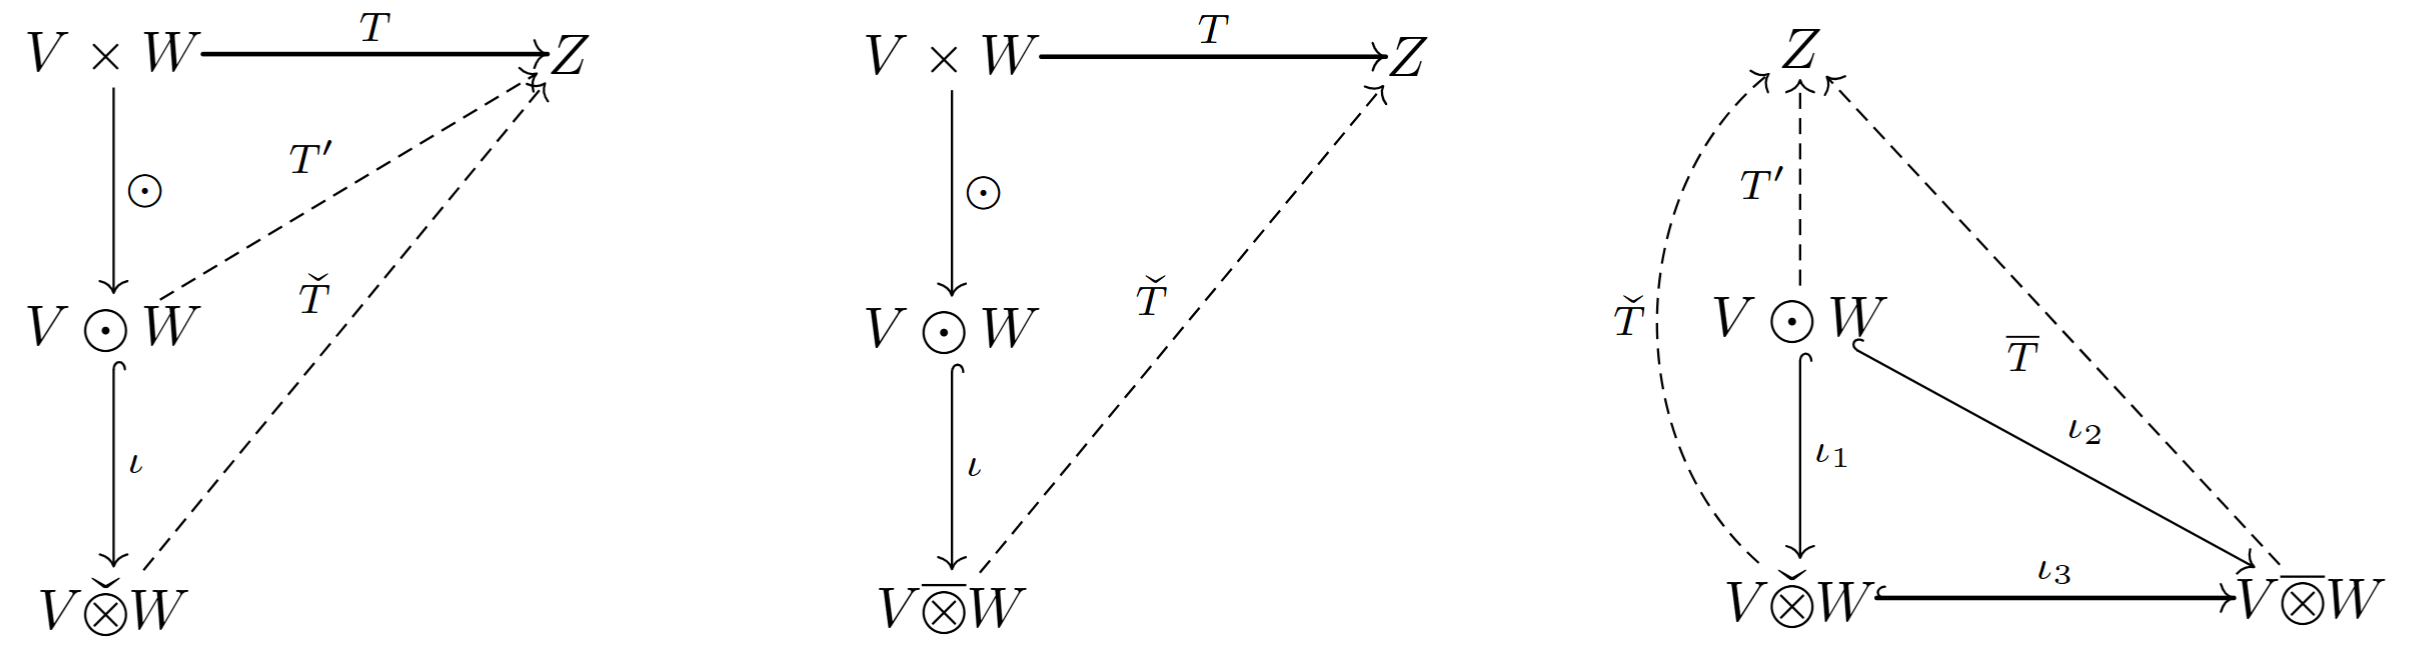
\includegraphics[width=1.0\textwidth]{images/Diagrama.png}
    \end{center}
\end{figure}

In the third diagram, we reason as follows:
from the first diagram above, we obtain $ \widecheck{T} \cdot \iota_1 = T =  \overline{T} \cdot \iota_2$, then, given that $\iota_2 = \iota_3 \cdot \iota_1$, we have  $ \widecheck{T} \cdot \iota_1 =  \overline{T} \cdot \iota_3 \cdot \iota_1$, from where if follows that $\overline{T} \circ \iota_3 = \widecheck{T}$.


We note that since \cite{sakaiCAlgebrasWAlgebras1998} and \cite{takesakiTheoryOperatorAlgebras1979} employ the standard completion, we may assume it satisfies the usual properties. 

\end{proof}

%$\cbnorm{\id \overline{\otimes} \Phi} =  \sup_{n} \opnorm{\id_{\SqMatrix{n}} \widecheck{\otimes} \id \overline{\otimes} \Phi} $


\todo[inline,size=\normalsize]{Ou Corolário ?}

\begin{proposition} \label{prop:cb_leq_wcb}
 Given a completely bounded normal map $\Phi:\mathscr{N}_1 \to \mathscr{N}_1 $, between $W^*$ algebras, it holds that:
 \[\cbnorm{\Phi} \leq \wcbnorm{\Phi}. \]
\end{proposition}

\begin{proof}
  This follows from \autoref{prop:opnorm_min_leq_wopnorm}, the definition of both norms (\autoref{def:cb_norm}, \autoref{def:wcb_nor}), the definition of \emph{supremum} as the least upper bound, and the fact that $\SqMatrix{n}$ is a $W^*$-algebra. We reason as follows,
\begin{equation*}
  \begin{split}
  \cbnorm{\Phi} & = \sup_{n} \opnorm{\id_{\SqMatrix{n}} \widecheck{\otimes} \Phi } \\
   & \leq \sup_{n} \opnorm{\id_{\SqMatrix{n}} \overline{\otimes} \Phi } & (\text{\autoref{prop:opnorm_min_leq_wopnorm}}) \\
   & \leq \sup_{\mathscr{M}} \opnorm{\id_{\mathscr{M}} \overline{\otimes} \Phi } = \wcbnorm{\Phi}.
    \end{split}
\end{equation*}
\end{proof}

\begin{comment}
\begin{corollary} \label{cor:cn_phi_leq_tensorid}
  Let $\Phi$ be a completely bounded normal map, it holds that,
  \[ \cbnorm{\id \overline{\otimes} \Phi}  \geq \cbnorm{\Phi}  \]
\end{corollary}

\begin{proof}
 With the previous result in hand, we have that 
\begin{equation}
  \begin{split}
    \cbnorm{\id \overline{\otimes} \Phi} = \sup_{n} \opnorm{\id_{\SqMatrix{n}} \widecheck{\otimes} \, (\id \overline{\otimes} \Phi)} \geq \sup_{n} \opnorm{\id_{\SqMatrix{n}} \widecheck{\otimes} \, (\id \widecheck{\otimes} \Phi)} = \cbnorm{ \Phi} 
  \end{split}
\end{equation}
\end{proof}
\end{comment}


\begin{proposition} \label{prop:cb_tensor_mult}
  Given normal completely positive maps  $\Phi$ and $\Psi$ between $W^*$-algebras, it holds that
  \[
  \opnorm{\phi \,\bar{\otimes} \, \psi} \leq \norm{\Phi} \norm{\Psi}.
\]
\end{proposition}

\begin{proof}
It follows directly from \autoref{thm:beta_alg_eq_beta_gamma} and 
\autoref{prop:norm_beta_alg}.
\end{proof}

\begin{corollary} \label{cor:cbnorm_tensor_leq_norm}
   Given a normal completely positive subunital map  $\Phi$ between $W^*$-algebras, it holds that
   \[
  \wcbnorm{\Phi} =\opnorm{\Phi}.
\]
\end{corollary}

\begin{proof}
  It follows from the proposition above and the definition of $W^*$ completely bounded norm (\autoref{def:wcb_nor}) that $\wcbnorm{\Phi} \leq \opnorm{\Phi}$. The inverse inequality follows from \autoref{prop:cb_leq_wcb} and the fact that $\|\phi\| = \|\phi\|_{\text{cb}}$ \cite[Exercise 11.5 (iii)]{pisierIntroductionOperatorSpace2003}.
\end{proof}

\begin{proposition} \label{prop:w*cb_submult}
  The $W^*$-completely bounded norm is submultiplicative with respect to composition for completely bounded normal maps between $W^*$-algebras. That is, given $W^*$-completely bounded normal maps $\Phi$ and $\Psi$ between $W^*$-algebras, we have:
  \[
    \wcbnorm{\Phi \cdot \Psi} \leq \wcbnorm{\Phi} \, \wcbnorm{\Psi}.
  \]
\end{proposition}

\begin{proof}
  It follows directly from the submultiplicativity of the operator norm (\autoref{lemma:op_norm_submult}), the
 definition of \emph{supremum} as the least upper bound, the definition of $W^*$ completely bounded norm,and the following property:
 for any two subsets $A$ and $B$ of only positive elements of an ordered field $\mathcal{F}$, let 
   $AB = \{ a \cdot b \, \mid \, a \in A, y \in B\},$
 it holds that $\sup A \cdot \sup B = \sup AB$
  \cite[Chapter 2, Section 8-9]{zakon2011mathematical}. Given the submultiplicativity of the operator norm, we have that each 
  \[a \in \{ \opnorm{ \id_{\mathscr{M}} \, \overline{\otimes} \, \Phi \cdot \Psi} \, \mid \, \mathscr{M} \text{ is a $W^*$ algebra} \} \] 
 has an upper bound 
  \[ b \in \{ \opnorm{ \id_{\mathscr{M}_1} \, \overline{\otimes} \, \Phi}   \opnorm{ \id_{\mathscr{M}_2} \, \overline{\otimes} \, \Psi}  \, \mid \, \mathscr{M_1}, \mathscr{M}_2 \text{ are $W^*$ algebras} \}.\]
 So, it follows from the definition of \emph{supremum} that,
  \[\sup_{\mathscr{M}} \{ \opnorm{ \id_{\mathscr{M}} \, \overline{\otimes} \, \Phi \cdot \Psi}\} \leq \sup_{\mathscr{M}_1, \mathscr{M}_2}   \{ \opnorm{ \id_{\mathscr{M}_1} \, \overline{\otimes} \, \Phi}   \opnorm{ \id_{\mathscr{M}_2} \, \overline{\otimes} \, \Psi} \} \]
 Consequently, applying the property stated at the beginning of the proof, it holds that,
 \[
    \wcbnorm{\Phi \cdot \Psi} \leq \wcbnorm{\Phi} \, \wcbnorm{\Psi}.
  \]
\end{proof}

\begin{proposition} \label{prop:cbnorm_id_otimes_phi}
   Given a $W^*$ completely bounded normal map $\Phi$ between $W^*$-algebras, it holds that
  \[
  \wcbnorm{\Phi \,\bar{\otimes} \, \id} \leq \wcbnorm{\Phi} \quad \text{and} \quad  \wcbnorm{\id\,\bar{\otimes} \, \Phi} \leq \wcbnorm{\Phi} .
\]
\end{proposition}

\begin{proof}
  \begin{comment}
  Given we just proved that the $W^*$ completely bounded norm is submultiplicative with respect to composition for $W^*$ completely bounded normal maps, it holds that
  \[
  \wcbnorm{\Phi \,\bar{\otimes} \, \id} = \wcbnorm{\sw \cdot (\id \,\bar{\otimes} \,\Phi)} \leq \wcbnorm{\sw} \wcbnorm{\id \,\bar{\otimes} \,\Phi}
  \]
By \autoref{prop:swap_nmiu} and \autoref{prop:miu_cp}, it follows that $\sw$ is a normal $\ast$-isomorphism, and, therefore, a completely positive normal map and an isometry (with respect to the operator norm). As a result, by \autoref{cor:cbnorm_tensor_leq_norm} and \autoref{prop:HomShortIsoIso}, we obtain $\wcbnorm{\sw} = \opnorm{\sw}=1$. 
\end{comment}
By \autoref{prop:swap_nmiu} it follows that $\sw$ is a normal $\ast$-isomorphism, and, therefore, an isometry (with respect to the operator norm). As a result,
\begin{align*}
  \wcbnorm{\Phi \,\bar{\otimes} \, \id} &= \sup_{\mathscr{M}} \opnorm{ \id_\mathscr{M} \, \overline{\otimes} \, \Phi \,\bar{\otimes} \, \id} \\
  & =  \sup_{\mathscr{M}} \opnorm{ \id_\mathscr{M} \, \overline{\otimes} \,  \sw \cdot (\id \,\bar{\otimes} \,\Phi)} \\
& = \sup_{\mathscr{M}} \opnorm{\id_\mathscr{M} \, \overline{\otimes} \,  \id \,\bar{\otimes} \,\Phi}  = \wcbnorm{\id \,\bar{\otimes} \,\Phi}. 
\end{align*}
At last, we need to prove that
\[
  \wcbnorm{\Phi \,\bar{\otimes} \, \id} \leq \wcbnorm{\Phi},
\]  
which follows direcly from the definition of the norm (\autoref{def:wcb_nor}) and the fact that the associator, $\alpha$, is an isometry with respect to the operator norm (\autoref{prop:assoc_nmiu}). 

%given the tensor product of $W^*$-algebras is itself a $W^*$-algebra \cite[Definition 5.1]{takesakiTheoryOperatorAlgebras1979}.
\end{proof}



\begin{comment}
We have established that either this norm coincides with the completely bounded norm, or the completely bounded norm is not suitable in this setting setting, since otherwise, there would exist a normal operator $\Phi$ between $W^*$-algebras and some $n \in \mathbb{N}$ such that
$
\cbnorm{\id_{\SqMatrix{n}} \overline{\otimes} \Phi} \geq \cbnorm{\Phi}.
$
Note that even if the two norms turn out to be equivalent, the use of this norm remains relevant, as it simplifies the demonstrations involved.
\end{comment}



%In this work, our focus is limited to showing that the metric induced by this norm makes $\WstarCPSUop$ into a first-order model. In future work, we aim to explore more deeply the relationship between this norm and the completely bounded norm, as well as to establish additional results that simplify distance computations between morphisms.





\begin{proposition} \label{prop:product_cb}
    Given $W^*$ completely bounded normal maps  $\Phi: \mathscr{M} \to \mathscr{N}_1$ and $\Psi: \mathscr{M} \to \mathscr{N}_2$ between $W^*$-algebras, it holds that
  \[
  \wcbnorm{\langle \Phi, \Psi \rangle} \leq \max \{\wcbnorm{\Phi}, \wcbnorm{\Psi}\}.
\]
\end{proposition}



\begin{proof}
  By \autoref{thm:w*_tensor_distributes_product}  and \autoref{def:c*_direct_sum} we have
  \begin{align*}
    &  \wcbnorm{\langle \Phi, \Psi \rangle}  = \sup_{\mathscr{T}} \opnorm{\id \, \overline{\otimes} \, \langle \Phi, \Psi \rangle} \\
    & \leq \sup_{\mathscr{T}} \opnorm{ \dist \cdot \id_\mathscr{T} \, \overline{\otimes} \, \langle \Phi, \Psi \rangle} & (\text{\autoref{thm:w*_tensor_distributes_product}}) \\
    &  \leq \sup_{\mathscr{T}} \opnorm{ \langle \id_\mathscr{T}\overline{\otimes} \Phi,\id_\mathscr{T}\overline{\otimes} \Phi  \rangle} &  \\
    & = \max \{ \sup_{\mathscr{T}} \opnorm{ \id_\mathscr{T}\overline{\otimes} \Phi}, \sup_{\mathscr{T}} \opnorm{ \id_\mathscr{T}\overline{\otimes} \Psi} \} & (\text{\autoref{def:c*_direct_sum}}) \\
    & \leq  \max \{  \wcbnorm{ \Phi} , \wcbnorm{\Psi}. \}
  \end{align*} 

  \begin{comment}
    By \autoref{thm:beta_alg_eq_beta_gamma}, \autoref{thm:w*_tensor_distributes_product}, and \autoref{def:c*_direct_sum} we have
  \begin{align*}
    & \hspace{-25pt} \wcbnorm{\langle \Phi, \Psi \rangle}  = \norm{\id \, \overline{\otimes} \, \langle \Phi, \Psi \rangle} \\
    & \hspace{-25pt} = \norm{\id  \odot \langle \Phi, \Psi \rangle} & (\text{Thm. \ref{thm:beta_alg_eq_beta_gamma}}) \\
    & \hspace{-25pt} = \sup_{s_i} \left\{ \norm{\id \odot \langle \Phi, \Psi \rangle \left(\sum_i s_i \otimes (m_i \otimes n_i)\right) } \Bigg| \norm{\sum_i s_i \otimes (m_i, n_i)}  = 1 \right\} \\
    & \hspace{-25pt} = \sup_{s_i} \left\{ \norm{ \sum_i( s_i \otimes \Phi(m_i), s_i \otimes \Phi(n_i) ) } \Bigg| \norm{\sum_i (s_i \otimes m_i, s_i \otimes n_i)}  = 1 \right\} & (\text{Thm. \ref{thm:w*_tensor_distributes_product}})\\
    & \hspace{-25pt} =  \sup_{\mathscr{S}}\left\{ \max \{\norm{\id_\mathscr{S} \odot \Phi},\norm{\id_\mathscr{S} \odot \Psi} \} \right\} & (\text{Def. \ref{def:c*_direct_sum}})\\
    & \hspace{-25pt} = \max \{  \sup_{\mathscr{S}} \id \, \overline{\otimes} \, \Phi, \sup_{\mathscr{S}} \id \, \overline{\otimes} \, \Psi  \}  & (\text{Thm. \ref{thm:beta_alg_eq_beta_gamma}}) \\
    &  \hspace{-25pt}\leq  \max \{  \wcbnorm{\id \, \overline{\otimes} \, \Phi} , \wcbnorm{\id \, \overline{\otimes} \, \Psi}  \}
  \end{align*} 
   \end{comment}
\end{proof}



\begin{theorem}
  $\WstarCPSUop$ is a distributive symmetric monoidal $\catMet$-category. 
\end{theorem}

\begin{proof}

  Firstly, note that the copairing in $\WstarCPSUop$ corresponds to the pairing in $\WstarCPSU$. As a result, by proof of \autoref{prop:Q_monoidal} and the definition of  symmetric monoidal $\catMet$-category, we need to prove that for any normal completely subunital maps $\Phi,\Phi',\Psi,\Psi' $ between $W^*$-algebras:
  \begin{enumerate}
    \item $\wcbnorm{(\Phi - \Phi')\Psi} \leq \wcbnorm{\Phi - \Phi'}  $ and  $\wcbnorm{\Phi'(\Psi - \Psi')} \leq \wcbnorm{\Psi - \Psi'}$. 
     Given these operadors are normal completely positive subunital and the $W^*$ completely bounded norm is submultiplicative with respect to composition for such maps, by \autoref{cor:cbnorm_tensor_leq_norm} and \autoref{prop:subunital_short} the inequalities hold.
     \item $\wcbnorm{\Phi \,\bar{\otimes} \, \id} \leq \wcbnorm{\Phi} \quad \text{and} \quad  \wcbnorm{\id\,\bar{\otimes} \, \Phi} \leq \wcbnorm{\Phi}$. It follows directly from \autoref{prop:cbnorm_id_otimes_phi}.
     \item $\wcbnorm{\langle \Phi - \Phi' , \Psi- \Psi' \rangle} \leq \max \{\wcbnorm{ \Phi - \Phi'}, \wcbnorm{\Psi- \Psi'}\}$. It follows directly from \autoref{prop:product_cb}.
  \end{enumerate}

\end{proof}



\begin{comment}

  
With the result above, we have established that the category $\WstarCPSUop$ is a suitable model for our $\lambda$-calculus. Consequently, we obtain a framework for reasoning about approximate equivalence in infinite-dimensional quantum computation. This, for example, enables us to reason about errors in quantum walks on a line \cite{venegasQuantumWalksComprehensive2012}.

Studying the Discrete Quantum Walk on a Line (DQWL) is important in quantum computation for several reasons:

\begin{enumerate}
    \item DQWL can be extended to construct quantum walks on more sophisticated structures, such as circles or general graphs.
    
    \item As a simple model, DQWL provides a valuable tool for exploring, identifying, and understanding fundamental properties of quantum walks that are crucial for developing quantum algorithms.
    
    \item DQWL serves as a testbed for verifying the quantumness of experimental implementations in quantum computing platforms.
\end{enumerate}
\end{comment}


\begin{comment}
\begin{definition} \cite[Introduction  p.4]{pisierTensorProductsCAlgebras2020} \label{def:cb_norm}
Let $\mathcal{A}$, $\mathcal{B}$ and $\mathcal{C}$ be $C^*$-algebras. Given  linear map $\phi: \mathcal{A} \to \mathcal{B}$ we define, we set
\[
\|\phi\|_{\text{cb}} = \sup_{\mathcal{C}} \|\id_{\mathcal{C}} \widecheck{\otimes} \phi\|.
\]
We call $\phi$ \emph{completely bounded} if $\|\phi\|_{\text{cb}} $ is finite.
Note that $\|\cdot\|_{\text{cb}}$ is a norm on the space of completely bounded maps. 
\end{comment}


%\mathscr{N}

%\cite[Prop. 3.5.2]{brownCalgebrasFinitedimensionalApproximations}
%motivação p/cb norm

%Fact 3.6.8 ([10, Prop. 3.5.2]). There exists a positive unital isometry f : A ! A such that f ⊙ idA : A ⊙ A ! A ⊙ A is unbounded (i.e. not norm-continuous). ◁


% \TraceOp{\HilbH}




%Here we draw attention to the fact that ...

%Eu estava a pensar na questão Selinger/Watrous. E gostaria de saber se podemos raciocinar da seguinte forma: O Watrous no que diz respeito à diamond / trace norm trabalha com mapas do tipo  Φ = L( H ) -> L( K), onde L(H) designa o espaço  dos mapas lineares de H para H. Ora, A = (A_1, A_2) ∈ C^{n×n} ⊕ C^{m×m}  pode ser visto com um mapa linear em L(C^n ⊕  C^m) definido como (A_1, A_2) (a,b) = (A_1(a), A_2(b)). Assim sendo, Φ:  C^{n_1×n_1} ⊕ C^{m_1×m_1} \-> C^{n_2×n_2} ⊕ C^{m_2×m_2} também pode ser visto como um mapa  Φ: L(C^n_1 ⊕  C^m_1) -> L(C^n_2 ⊕  C^m_2) e, portando, o "casamento Selinger/Watrous" é automático: podemos usar a diamond norm diretamente nos mapas Φ do Selinger. No caso de esta linha de racicionio não estar correta, pedia que, se possível, marcássemos uma reunião online ainda esta semana, porque parece-me que definir a norma de um mapa Φ do Selinger com base na diamond norma de somas diretas de mapas Φ_i:  L( H ) -> L( K), levanta alguns problemas.

%\( \iota: A \xhookrightarrow{\text{inc}} B \)



\section{Examples}

We now illustrate the use of (first-order) $\lambda$-calculus with conditionals for describing quantum
programs. To this effect, we first consider a type $\mathtt{qbit}$ of qubits, the
basic unit of information in quantum computation. We then regard $\typeI \oplus
\typeI$ to be the type of bits. Next, we propound the following
basic quantum operations:  the conversion of a bit into a qubit, $q : \typeI
\oplus \typeI  \to \mathtt{qbit}$, the measurement of a qubit,
$\emph{meas}:\mathtt{qbit} \to \typeI \oplus \typeI$, and pre-determined sets of
operations on $n$-qubits, $\emph{U},\emph{CPTP}:\mathtt{qbit},\ldots,\mathtt{qbit} \to
\mathtt{qbit}^{\otimes n}$. The former includes unitary operations, as the Hadamard
gate $H : \mathtt{qbit} \to \mathtt{qbit}$, the not-gate $X : \mathtt{qbit} \to
\mathtt{qbit}$, and the cnot-gate $CNOT : \mathtt{qbit},\mathtt{qbit} \to
\mathtt{qbit}^{\otimes 2}$, and the latter set includes operations such as dephasing with probability $p$, $D_p : \mathtt{qbit},\mathtt{qbit} \to
\mathtt{qbit}^{\otimes 2}$. We consider as well a pre-determined set of quantum
states $\ket{\psi} : \typeI \to \mathtt{qbit}$ and a discard operation $\text{disc}: \mathtt{qbit} \to \typeI$.  

$\catQ$ forms a model of the metric $\lambda$-theory for quantum computation via the following interpretation: $\sem{\typeI}= \mathbb{C} \ni  1$, 
$\sem{\mathtt{qbit} \hspace{1pt}}= \mathbb{C}^{2\times2}$, 
$\sem{\emph{q} \hspace{1pt}}((a,b)) = \big(\begin{smallmatrix}
  a & 0\\
  0 & b
\end{smallmatrix}\big)$, 
 $\sem{\ket{\psi}} (1)= \ket{\psi} \bra{\psi}$,
$\sem{\emph{meas} \hspace{1pt}} (\rho)= (\text{Tr} (M_{0} \rho M_{0}^{\dag}), \text{Tr} (M_{1} \rho M_{1}^{\dag}))$, and $\sem{\text{disc}} (\rho)= \tr (\rho)$.
For unitary operations $U$ we define $\sem{U}= U \rho U^{\dag}$.
For completely positive trace-preserving operators $\emph{CPTP}$, defined as $\emph{CPTP} (\rho) = \sum_i K_i \rho K_i^{\dag}$, we define  $\sem{\emph{CPTP}} = \emph{CPTP}(\rho)$.

Let us now apply this machinery to two well-known problems in quantum computation
and quantum information.

\subsection{Quantum state discrimination}


\begin{example} [Coin-Toss]
  In the quantum setting, tossing a ``fair'' coin can be described as preparing a qubit in a superposition of two states, $\ket{0}$ and $\ket{1}$, representing `heads' and `tails', each with an equal probability of $0.5$ and then measuring it. This is achieved by simply applying a Hadamard gate to the initial state $\ket{0}$, followed by a measurement.
More generally, tossing a coin (whether ``fair'' or ``unfair'') can be described as preparing a qubit in a superposition of  $\ket{0}$ and $\ket{1}$, with probabilities $p$ and $1-p$, respectively,  and then measuring it.  Considering $p= \cos(\theta/2)^2$ and the quantum gate $R_{y,\theta} : \mathtt{qbit} \to \mathtt{qbit}$, representing a single-qubit rotation by an angle \( \theta \) around the y-axis,  this process is described by the following $\lambda$-term:
\begin{align*}
  &\textbf{CoinToss} = - \vljud \emph{meas} (R_{y,\theta} (\ket{0})): \typeI \oplus \typeI
\end{align*}

When running a quantum program on a real quantum computer, the quantum circuits are mapped to the hardware's native quantum gates during compilation. For instance consider 2020 IBM's native quantum gate set $U_1,U_2,U_3,CX$ \cite{December2020Product} where

  \begin{align*}
    U_1(\lambda) &= 
    \begin{pmatrix}
        1 & 0 \\
        0 & e^{i\lambda}
    \end{pmatrix} \\
    U_2(\phi, \lambda) &= 
    \frac{1}{\sqrt{2}}
    \begin{pmatrix}
        1 & -e^{i\lambda} \\
        e^{i\phi} & e^{i(\phi+\lambda)}
    \end{pmatrix} \\
    U_3(\theta, \phi, \lambda) &= 
    \begin{pmatrix}
        \cos(\theta/2) & -e^{i\lambda}\sin(\theta/2) \\
        e^{i\phi}\sin(\theta/2) & e^{i(\phi+\lambda)}\cos(\theta/2)
    \end{pmatrix} \\
\end{align*}

Here, \( R_{y,\theta} \), can be expressed as \( U_3(\theta, 0, 0) \). We now examine how the coin toss outcome is affected when the \( U_3 \) gate is faulty, particularly when its parameter \( \theta \) is perturbed by an error \( \epsilon \). In this case, the implemented gate becomes \( U_3(\theta + \epsilon, \phi, \lambda) \), \ie, $R_{y,\theta+\epsilon}$.
First, we compute the action of the unitary operator \( U_3(\theta, \phi, \lambda) \) on an arbitrary quantum state \( \ket{\psi} \).
\begin{align*}
  U_3(\theta, \phi, \lambda) \ket{\psi} 
  & = U_3(\theta, \phi, \lambda) \left(\cos(\alpha/2) \ket{0} + e^{i\beta}\sin(\alpha/2) \ket{1} \right)\\
  & = \left(\cos(\alpha/2) \cos(\theta/2) - e^{i (\lambda + \beta)}  \sin(\alpha/2)\sin(\theta/2) \right) \ket{0} \\
  & + \left(e^{i \phi}\cos(\alpha/2)\sin(\theta/2) + e^{i (\beta + \lambda + \phi)} \sin(\alpha/2) \cos(\theta/2 ) \right) \ket{1}
\end{align*}
Designating $U_3(\theta, \phi, \lambda) \ket{\psi} = a \ket{0} + b \ket{1}$, one has
\begin{align*}
  \hspace{-25pt} a a^* &= \vert \cos(\alpha/2) \cos(\theta/2) - e^{i (\lambda + \beta) }  \sin(\alpha/2)\sin(\theta/2) \vert ^2 \\
  \hspace{-25pt} & = \cos^2(\alpha/2) \cos^2(\theta/2) - 2 \cos(\beta + \lambda) \cos(\alpha/2) \cos(\theta/2)  \sin(\alpha/2)\sin(\theta/2)  \\
  \hspace{-25pt} & \hspace{10pt} + \sin(\alpha/2)^2 \sin^2(\theta/2) \\
  \hspace{-25pt} & = \cos^2(\alpha/2) \cos^2(\theta/2) + \sin^2(\alpha/2) \sin^2(\theta/2)  - 1/2 \cos(\beta + \lambda) \sin(\alpha)\sin(\theta) \\
  \hspace{-25pt} & = \cos^2((\theta+\alpha)/2)+(1-\cos(\beta + \lambda))\sin(\alpha)\sin(\theta) -1 \\
  \hspace{-25pt} a^*b & = \left(\cos(\alpha/2) \cos(\theta/2) - e^{-i (\lambda + \beta)}  \sin(\alpha/2)\sin(\theta/2) \right) \big(e^{i \phi}\cos(\alpha/2)\sin(\theta/2) \\
  \hspace{-25pt} & \hspace{10pt}  + e^{i (\beta + \lambda + \phi)} \sin(\alpha/2) \cos(\theta/2 ) \big) \\
  \hspace{-25pt} & = (1/2) \big( e^{i \phi} \cos^2(\alpha/2) \sin(\theta) + e^{i (\beta + \lambda + \phi)} \sin(\alpha) \cos^2(\theta/2) - e^{-i (\beta + \lambda -\phi)} \sin(\alpha) \sin^2(\theta/2) \\
  \hspace{-25pt} & \hspace{10pt}  - e^{i \phi} \sin^2(\alpha/2) \cos(\theta/2)  \big) \\
  \hspace{-25pt} & = (1/2) \left( e^{i \phi}\cos(\alpha) \sin(\theta) +  \sin(\alpha) \left(e^{i (\beta + \lambda + \phi)} \cos^2(\theta/2) - e^{-i (\beta + \lambda - \phi)} \sin^2(\theta/2)\right)  \right)
\end{align*}
Then, we calculate the vector Bloch of $U_3(\theta, \phi, \lambda) \ket{\psi}$,
\begin{align*}
  &x = 2 \text{Im} \left( a^{*}b \right) =   \cos(\phi) \cos(\alpha) \sin(\theta) +  \sin(\alpha) \big(\cos{(\beta + \lambda + \phi)} \cos^2(\theta/2) \\
  & \hspace{10pt} - \cos{(\beta + \lambda - \phi)} \sin^2(\theta/2)\big)  \\
  &y = 2 \text{Re} \left( a^{*}b \right) = \sin(\phi) \cos(\alpha) \sin(\theta) +  \sin(\alpha) \big(\sin{(\beta + \lambda + \phi)} \cos^2(\theta/2) \\
  & \hspace{10pt} + \sin{(\beta + \lambda - \phi)} \sin^2(\theta/2)\big) \\
  & z = 2 aa^* -1 = 2 \cos^2((\theta+\alpha)/2)+(1-\cos(\beta + \lambda))\sin(\alpha)\sin(\theta) -1
\end{align*}
As a result, we have,
\begin{align*}
  & \tracenorm{U_3(\theta, 0, 0) \ket{\psi}\bra{\psi} U_3(\theta, 0, 0)^\dag - U_3(\theta + \epsilon, 0, 0) \ket{\psi}\bra{\psi}U_3(\theta+\epsilon, 0, 0)^\dag } \\
  & = \lVert ( \cos(\alpha) (\sin(\theta) - \sin(\theta + \epsilon)) +  \sin(\alpha) \cos{\beta} \left(\cos(\theta) - \cos(\theta + \epsilon) \right) , 0,\\
  & \hspace{20pt} 2 (\cos^2((\theta+\alpha)/2) - \cos^2((\theta+ \epsilon+\alpha)/2))+\cos(\beta) \sin(\alpha)(\sin(\theta) - \sin(\theta+\epsilon)) )\rVert_2 \\
  %& \leq \lVert  (\sin(\theta) - \sin(\theta + \epsilon) + \cos(\theta) - \cos(\theta + \epsilon),0, \\
  %&  \hspace{20pt}  2 (\cos^2((\theta+\alpha)/2) - \cos^2((\theta+ \epsilon+\alpha)/2))+(\sin(\theta) - \sin(\theta+\epsilon))) \rVert_2   \\
  &  \leq \euclideannorm{( \cos(\alpha)\epsilon + \sin(\alpha)\cos(\beta) \epsilon, 0, 2\epsilon + \sin(\alpha)\cos(\beta) \epsilon)} \\
  & = \sqrt{\epsilon^2(\cos^2(\alpha) + 2\sin^2(\alpha)\cos^2(\beta)+\sin(2\alpha)\cos(\beta) + 2\sin(\alpha)\cos(\beta) + 4 )} \\
  &\leq \epsilon \sqrt{(1 + \sin^2(\alpha) +\sin(2\alpha) + 2\sin(\alpha) + 4 )} \\
  & \leq \epsilon \sqrt{(1 + 4 + 4 )} = 3 \epsilon
\end{align*}

The first inequality arises from both functions $\cos$ and $\sin$ being Lipschitz continuous. Attending to \autoref{theorem:diamond_iso}, it follows that
  \begin{align*}
    \diamondnorm{R_{y, \theta}- R_{y, \theta + \epsilon} } \leq 3 \epsilon
  \end{align*}

Using our metric deductive system, we can easily conclude that $\textbf{CoinToss} =_{3 \epsilon} \textbf{CoinToss}^{\epsilon}$, where $\textbf{CoinToss}^{\epsilon}$ is the the judgement that results from replacing $R_{y, \theta}$ by $R_{y, \theta + \epsilon}$.

\end{example}


\begin{example}[Quantum state discrimination] \label{ex:quantum_state_discrimination_syntax}
Quantum state discrimination is a pivotal challenge in 
 quantum communications \cite{barnett2009qinfo,watrous2018theory} and quantum cryptography \cite{Gisin02qcripto}. 
While orthogonal states can be perfectly distinguished, the same does not apply
to nonorthogonal states. In fact, even when the set of possible nonorthogonal
states is known, determining the optimal discrimination strategy is considered
a nontrivial problem.

The problem of quantum state discrimination can be naturally introduced through its connection with quantum communication. Consider two parties, Alice and Bob, who want to communicate with each other using a quantum channel. Alice chooses a state from a known set $\{\ket{\psi_i}\}$, each occurring with a known probability $p_i$, and sends it to Bob through the channel. Bob, who knows both the set of possible states and their associated probabilities, performs a suitable measurement to determine which state Alice sent. This scenario defines the quantum state discrimination problem: how to optimally distinguish between a known set of quantum states, each prepared with a known prior probability $p_i$.

When distinguishing between two pure states, the optimal measurement known as the \emph{Helstrom measurement} is given by a projective measurement
\cite{barnett2009qinfo}.  When operating within the computational basis, a
projective measurement can be understood as the application of a unitary
operator followed by a subsequent measurement in the computational basis. Thus,
the optimal measurement can be interpreted as a unitary transformation applied
to the quantum state, followed by a measurement in the computational basis. 

We will now show how to describe this discrimination task in
$\lambda$-calculus.  Consider two pure states $\ket{\psi_0}$ and
$\ket{\psi_1}$, prepared \emph{a priori} with probabilities $p_0$ and $p_1 = 1-p_0$,
respectively. Consider as well an operation $U : \mathtt{qbit} \to \mathtt{qbit}$ which
corresponds to the basis-change associated with the optimal measurement.
The relevant $\lambda$-terms are then:
\begin{align*}
  &\textbf{StatePreparation} =  b: \typeI \oplus \typeI  \vljud  \text{case } b\,
  \{\inl_{\typeB}(x) \Rightarrow \ket{\psi_0} ; \inr_{\typeA}(y) \Rightarrow \ket{\psi_1}\}: \mathtt{qbit} \\
  &\textbf{HMeasure} =  x : \mathtt{qbit} \vljud \emph{meas} (\emph{U}(x)): \typeI \oplus \typeI \\
  %&\textbf{Discrimination} = (p_0,p_1): \typeI\oplus \typeI \vljud \textbf{HMeasure} [ \textbf{StatePreparation} [(p_0,p_1)/ b] / x] : \typeI\oplus \typeI
  &\textbf{Discrimination} = - \vljud \textbf{HMeasure} [ \textbf{StatePreparation} [\textbf{CoinToss}(*)/ b] / x] : \typeI\oplus \typeI
\end{align*}

An arbitrary single qubit unitary $U \in \mathbb{C}^{2 \times 2}$ may be written
\[
U = e^{i\alpha} R_{z,\beta} R_{y,\gamma} R_{z,\delta},
\]
for appropriate choices of angles $\alpha$, $\beta$, $\gamma$ and $\delta$.


As in the previous example, we assume the hardware's native gate set consists of $\{U_1, U_2, U_3,$ $ \text{CNOT}\}$, and the quantum circuit is compiled into these gates.  
As previously noted, the $R_y(\theta)$ gate can be implemented as $U_3(\theta, 0, 0)$.  
Similarly, the $R_z(\lambda)$ gate is equivalent to $U_1(\lambda)$ up to a global phase factor $e^{-i\lambda/2}$, consequently, it can be directly implemented using this gate.  
We will also consider that the gates $U_1$ and $U_3$ are affected by errors $\epsilon_1$ and $\epsilon_2$, respectively. 
More precisely, we will consider erroneous implementations of this gates $U_1(\lambda + \epsilon_1)$ and $U_3(\theta + \epsilon_2, \phi, \lambda)$. 
From the previous example, we know that the error in the $R_y$ gate is bounded by $3 \epsilon_2$. 
Consider the single-qubit state
\[
\ket{\psi} = \cos\left(\frac{\alpha}{2}\right)\ket{0} + e^{i\beta}\sin\left(\frac{\alpha}{2}\right)\ket{1}.
\]
Applying the \( U_1(\lambda) \) gate yields
\[
U_1(\lambda)\ket{\psi} = \cos\left(\frac{\alpha}{2}\right)\ket{0} + e^{i(\beta + \lambda)}\sin\left(\frac{\alpha}{2}\right)\ket{1}.
\]
The corresponding Bloch vector is then
\[
\left(\!\cos(\beta + \lambda)\sin\alpha,\; \sin(\beta + \lambda)\sin\alpha,\; \cos\alpha\right).
\]
Consequently, applying the same reasoning as in the previous example, it follows that
\begin{align*}
  & \hspace{-15pt} \tracenorm{U_1(\lambda) \ket{\psi}\bra{\psi} U_1(\lambda)^\dag - U_1(\lambda + \epsilon_1) \ket{\psi}\bra{\psi}U_1(\lambda + \epsilon_1)^\dag } \\
  & \hspace{-15pt} = \euclideannorm{\left(\sin(\alpha) \left( \cos(\beta + \lambda) -  \cos(\beta + \lambda + \epsilon_1) \right),\sin(\alpha) \left( \sin(\beta + \lambda) -  \sin(\beta + \lambda + \epsilon_1) \right),0 \right)} \\
  & \hspace{-15pt}\leq \euclideannorm{\left( \cos(\beta + \lambda) -  \cos(\beta + \lambda + \epsilon_1) , \sin(\beta + \lambda) -  \sin(\beta + \lambda + \epsilon_1) ,0 \right)} \\
  & \hspace{-15pt} \leq \euclideannorm{\left( \epsilon_1, \epsilon_1 ,0 \right)} \\
  & \hspace{-15pt} = \sqrt{2}\epsilon_1 
\end{align*} 

Attending to \autoref{theorem:diamond_iso}, it follows that
  \begin{align*}
    \diamondnorm{U_1(\lambda)- U_1(\lambda + \epsilon_1) } \leq \sqrt{2} \epsilon_1.
  \end{align*}

Given the erroneous $R_y$ gate is bounded by $3 \epsilon_2$, we observe that the $R_y$ gate amplifies errors more significantly than the $R_z$ gate for errors of the same magnitude.


As a result, considering the $\lambda$-term \textbf{HMeasure} and the erroneous implementation of $U$ described above, denoted $U^{\epsilon_1, \epsilon_2}$, using our deductive metric system, we have $U =_{\sqrt{2}\epsilon_1+ 3\epsilon_2} U^{\epsilon_1, \epsilon_2}$. This equation implies that if $\epsilon_1 = \epsilon_2$, the erroneous $U_3$ gate contributes more than twice as much as the erroneous $U_1$ gate to the upper bound on the total distance between the ideal and erroneous unitary.

Next, we deduce $\textbf{HMeasure} =_{\sqrt{2}\epsilon_1+ 3\epsilon_2} \textbf{HMeasure}^{\epsilon_1, \epsilon_2}$, where $\textbf{HMeasure}^{\epsilon_1, \epsilon_2}$ is the the judgement that results from replacing $U$ by $U^{\epsilon_1, \epsilon_2}$.
Moreover, considering the erroneous implementation of the $R_y$ gate also afecting the \textbf{CoinToss} term, as discussed in the previous example, we deduce that 
$$\textbf{Discrimination} =_{\sqrt{2}\epsilon_1+6\epsilon_2} \textbf{Discrimination}^{\epsilon_1,\epsilon_2}, $$
where $\textbf{Discrimination}^{\epsilon_1,\epsilon_2}$ denotes the judgement that results from replacing $\textbf{HMeasure}$ by $\textbf{HMeasure}^{\epsilon_1, \epsilon_2}$ and $\textbf{CoinToss}$ by  $\textbf{CoinToss}^{\epsilon_2}$.

Observe that the distance between the ideal and erroneous quantum state discrimination tends to $0$ as $\epsilon_1$ and $\epsilon_2$ tend to zero, as expected. 
Additionally, since an erroneous $U_3$ gate affects both \textbf{HMeasure} and \textbf{CoinToss}, we find that when $\epsilon_1$ and $\epsilon_2$ are of equal magnitude, the erroneous $U_3$ contributes more than four times as much as the erroneous $U_1$ to the upper bound on the total distance between the ideal and erroneous unitary.



\end{example}


\subsection{Quantum teleportation protocol}


\label{ex:quantum_teleportation_syntax}
\cite{bennett1993teleporting} introduced the concept of quantum teleportation,
a protocol that allows the transfer of  unknown quantum states between distant
parties.  The quantum teleportation protocol is a fundamental building block of
quantum communication, quantum computation, and quantum networks, its
applications ranging from secure quantum communication to distributed quantum
computing
\cite{briegel1998quantum,gottesman1999demonstrating,kimble2008quantum}.

Conceptually it can be described as follows: Alice and Bob share an entangled
pair of qubits, specifically in a Bell state. Alice keeps the first qubit and
Bob the second. Moreover, Alice has a qubit in an unknown state $\ket{\psi}$
that she wants to send to Bob.  Alice entangles her qubit and the first qubit
in the Bell state, and then measures both. The result of this measurement is
two classical bits that Alice then sends to Bob though a classical channel.
Based on the measurement results, Bob applies a correction to his qubit so it
matches the initial state $\ket{\psi}$.  The circuit corresponding to the
implementation of quantum teleportation is depicted in \autoref{fig:teleport}.


\begin{figure} [H]
  \centering
  \begin{quantikz} [column sep=0.2cm, row sep=0.5cm] 
      \lstick{$\ket{\psi}$}  & \qw &\qw & \qw & \qw & \qw& \ctrl{1}\gategroup[2,steps=4,style={dashed,rounded
      corners,fill=blue!20, inner
      xsep=2pt},background,label style={label
      position=below,anchor=north,yshift=-0.2cm}]{{\sc
      BellMeasure}} & \gate{H} & \qw & \meter{} & \setwiretype{c}  &  & \gategroup[3,steps=4,style={dashed,rounded
      corners,fill=blue!20, inner
      xsep=2pt},background,label style={label
      position=below,anchor=north,yshift=-0.2cm}]{{\sc
      Correction}}  &  & & \ctrl[vertical
wire=c]{2}  \\
      \lstick {$\ket{0}$}  &\gate{H}\gategroup[2,steps=3,style={dashed,rounded
      corners,fill=blue!20, inner
      xsep=2pt},background,label style={label
      position=below,anchor=north,yshift=-0.2cm}]{{\sc
      EPR}} & \qw  & \ctrl{1}& \qw & \qw & \targ{} & \qw & \qw & \meter{} & \setwiretype{c} & & & \ctrl[vertical
wire=c]{1} \\
      \lstick{$\ket{0}$}  &  \qw & \qw &  \targ{} & \qw &\qw&\qw & \qw & \qw& \qw & \qw & \qw &  \qw & \gate{X} & \qw & \gate{Z} 
 \end{quantikz}
  \caption{Quantum Teleportation Protocol}
  \label{fig:teleport}
\end{figure}
We first describe each of the rectangles filled in blue separately, and using
standard quantum gate operations, namely $H: \mathtt{qbit} \to \mathtt{qbit}$, $X:
\mathtt{qbit} \to  \mathtt{qbit}$, $Z: \mathtt{qbit} \to \mathtt{qbit}$, and
$\emph{CNOT}: \mathtt{qbit}, \mathtt{qbit} \to \mathtt{qbit} \otimes \mathtt{qbit}$:
\begin{align*}
   & \hspace{-25pt} \textbf{EPR} =  \emph{CNOT} (\emph{H}\ket{0},\ket{0}) : \mathtt{qbit} \otimes
   \mathtt{qbit}  \\ 
   %
   &\hspace{-25pt}\textbf{BellMeasure} =  q_{1}: \mathtt{qbit}, q_{2}: \mathtt{qbit}
   \vljud  \text{pm} \, \textit{CNOT} (q_{1},q_{2})
  \,  \text{to}\, x \otimes y. \,
    \\
   & \hspace{150pt} \textit{meas} (\textit{H} (x)) \otimes \textit{meas} (y) : \left(\typeI\oplus \typeI\right) \otimes \left(\typeI\oplus
   \typeI\right) \\
   %
   &\hspace{-25pt}\textbf{Correction}= q: \mathtt{qbit}, x: \typeI \oplus \typeI,  y:
        \typeI \oplus \typeI \, \vljud \\
    &\hspace{50pt} \text{case } x \left\{ 
        \begin{aligned} 
          & \inl (x_{0}) \Rightarrow x_0 \text{ to } \ast. \text{case } y \left\{
                \begin{aligned}
                  &\inl (y_{0})  \Rightarrow  y_0 \text{ to } \ast.
                        \, q; \\
                  &\inr (y_{1}) \Rightarrow y_1 \text{ to } \ast. \, \emph{X}
                \end{aligned} \right\}; \\
          & \inr (x_{1})  \Rightarrow x_1 \text{ to } \ast. \text{case } y \left\{
                \begin{aligned}
                  &  \inl (y_{0})  \Rightarrow
        y_0 \text{ to } \ast. \, \emph{Z}(q); \\
                  &\inr (y_{1}) \Rightarrow{} y_1 \text{ to } \ast. \, \emph{Z}
(\emph{X}(q))
                \end{aligned} \right\}
        \end{aligned}\right\} : \mathtt{qbit}
\end{align*}

Designating the qubit to be teleported as $qb_0$, one then describes the
teleportation procedure in $\lambda$-calculus as follows:
 \begin{align*}
  \textbf{QTP} = qb_{0}: \mathtt{qbit}\hspace{3 pt} \vljud \hspace{3 pt} & \text{pm} \hspace{5pt} \textbf{EPR} \hspace{5pt} \text{to} \hspace{5pt}  qb_{1} \otimes qb_{2}.  \notag \\
     & \text{pm}\hspace{5pt} \textbf{BellMeasure}\, [qb_0/q_1,qb_{1}/q_2] \hspace{5pt}  \text{to} \hspace{5pt} c_{0}\otimes c_{1} . \notag \\
     & \textbf{Correction}\, [qb_{2}/q,c_{0}/x, c_{1}/y] 
     : \mathtt{qbit} 
 \end{align*}


 Following the approach of previous examples, we analyze erroneous implementations of the gates $U_1$ and $U_3$ within the hardware’s native gate set. Additionally, we consider the action of both dephasing and amplitude damping channels. Furthermore, we account for an adversarial agent that applies a bit-flip operation immediately prior to measurement with probability $ p = 0.5 $.  

    Here, we consider imperfect implementations of the gates $U_1$ and $U_3$, given by $ U_1(\lambda + \epsilon_1) $ and $ U_3(\theta, \phi + \epsilon_2, \lambda + \epsilon_3)$, respectively. 
    Recall from the previous example that we established the upper bound $\diamondnorm{U_1(\lambda)- U_1(\lambda + \epsilon_1) } \leq \sqrt{2} \epsilon_1$.
     The Hadamard gate, $H$, is the composition $U_3(\pi/2, 0, 0)\cdot U_1(\pi)$. We calculate,
    \begin{align*}
      &\tracenorm{U_3(\pi/2, 0, 0) \ket{\psi}\bra{\psi}U_3(\pi/2, 0, 0)^\dag - U_3(\pi/2, \epsilon_2, \epsilon_3)  \ket{\psi}\bra{\psi}U_3(\pi/2, \epsilon_2, \epsilon_3)^\dag} \\
      & = \lVert (\cos(\alpha)( 1-\cos{\epsilon_2}) + \sin(\alpha)( 1/2(\cos(\beta + \epsilon_2 + \epsilon_3)-\cos(\beta - \epsilon_2 + \epsilon_3))), \\
      & \hspace{20pt} \cos(\alpha)( 1-\sin{\epsilon_2}) + (1/2)\sin(\alpha) (\sin(\beta)-\sin(\beta+\epsilon_2 + \epsilon_3)   \\
      & \hspace{20pt} + \sin(\beta)-\sin(\beta-\epsilon_2 + \epsilon_3)),  (\cos(\beta + \epsilon_3)-\cos(\beta))\sin(\alpha) ) \lVert_2 \\
      & \leq ||(\cos(\alpha) \epsilon_2 + (1/2)\sin(\alpha) (\epsilon_2 + \epsilon_3) ,\cos(\alpha) \epsilon_2 + (1/2)  \sin(\alpha) (\epsilon_2 + \epsilon_3 + |\epsilon_3-\epsilon_2|), \\
      & \hspace{20pt} \sin(\alpha) \epsilon_3)||_2 \\
      &  < \euclideannorm{(\epsilon_2 + (1/2)(\epsilon_2 + \epsilon_3), \epsilon_2 + (1/2)   (\epsilon_2 + \epsilon_3 + |\epsilon_3-\epsilon_2|), \epsilon_3)}  \\
      & \leq 3 \epsilon_2 +  2\epsilon_3 + |\epsilon_2-\epsilon_3| \\
    \end{align*}

    Attending to \autoref{theorem:diamond_iso}, it follows that
    \begin{align*}
      \diamondnorm{U_3(\pi/2, 0, 0)- U_3(\pi/2, \epsilon_2, \epsilon_3) } \leq 3 \epsilon_2 +  2\epsilon_3 + |\epsilon_2-\epsilon_3|
    \end{align*}

    
    As a result, denoting the imperfect implementation of the Hadamard gate as $H^{\epsilon_1 ,\epsilon_2, \epsilon_3}$, we have 
    \begin{align} \label{eq:h_error_telepor}
      H =_{ \sqrt{2}\epsilon_1 + 3 \epsilon_2 + 2\epsilon_3 + |\epsilon_2-\epsilon_3|} H^{\epsilon_1 ,\epsilon_2, \epsilon_3}.
    \end{align}
 

    The gate $X$ can be implemented as $U_3(\pi, 0, \pi)$. We compute,
    \begin{align*}
      &\tracenorm{U_3(\pi, 0 , \pi) \ket{\psi}\bra{\psi}U_3(\pi,0,\pi)^\dag - U_3(\pi,\epsilon_2,\pi+\epsilon_3)  \ket{\psi}\bra{\psi}U_3(\pi,\epsilon_2,\pi+\epsilon_3)^\dag}  \\
      & =\euclideannorm{( \sin(\alpha) (\cos(\beta)+\cos(\beta + \epsilon_3-\epsilon_2)), \sin(\alpha) (\sin(\beta + \epsilon_3-\epsilon_2)-\sin(\beta)),0 )} \\
      &  \leq \euclideannorm{(|\epsilon_3-\epsilon_2|, |\epsilon_3-\epsilon_2|,0 )} \\
      & = \sqrt{2} |\epsilon_3-\epsilon_2|
    \end{align*}

   Recall that the gate $U_3$ is defined as
\begin{align*}
    U_3(\theta, \phi, \lambda) &= 
    \begin{pmatrix}
        \cos(\theta/2) & -e^{i\lambda}\sin(\theta/2) \\
        e^{i\phi}\sin(\theta/2) & e^{i(\phi+\lambda)}\cos(\theta/2)
    \end{pmatrix}.
\end{align*}
Thus, when $\epsilon_2 = \epsilon_3 = \epsilon$, the unitaries $U_3(\pi, 0, \pi)$ and $U_3(\pi, \epsilon_2, \pi + \epsilon_3)$ differ only by a global phase factor $e^{i\epsilon}$. Therefore, it is reasonable for the distance between $X$ and its erroneous version to tend to $0$ as $|\epsilon_3 - \epsilon_2|$ tends to $0$.

    Considering \autoref{theorem:diamond_iso}, it holds that
    \begin{align*}
      \diamondnorm{U_3(\pi, 0 , \pi)- U_3(\pi,\epsilon_2,\pi+\epsilon_3) } \leq \sqrt{2} |\epsilon_3-\epsilon_2|
    \end{align*}

    As a result, denoting the erroneous implementation of the $X$ gate as $X^{\epsilon_2, \epsilon_3}$, we have
    \begin{align} \label{eq:x_error_telepor}
      X =_{\sqrt{2} |\epsilon_3-\epsilon_2|} X^{\epsilon_2, \epsilon_3}.
    \end{align}
  

    Finally, the gate $Z$ corresponds to $U_1(\pi)$, therefore, denoting the erroneous implementation of the $X$ gate as $X^{\epsilon_1}$, we postulate the following axiom
    \begin{align} \label{eq:z_error_telepor}
      Z =_{\sqrt{2} \epsilon_1} Z^{\epsilon_1}.
    \end{align}

    Designating the \textbf{Correction} block with the imperfect implementations of $X$ and $Z$ by $\textbf{Correction}^{\epsilon_1, \epsilon_2, \epsilon_3}$, in light of the axioms in equations \eqref{eq:x_error_telepor} and \eqref{eq:z_error_telepor} and our metric deductive system we have that
    \begin{align} \label{eq:correction_error_telepor}
      \textbf{Correction} =_{\sqrt{2} \left(\epsilon_1 +|\epsilon_3-\epsilon_2| \right)} \textbf{Correction}^{\epsilon_1, \epsilon_2, \epsilon_3}.
    \end{align}


    We observe, as expected and in light of our previous remark regarding the upper bound on the distance between $X$ and its erroneous version, that when both the error of the $U_1$ gate, $\epsilon_1$, and the absolute difference between the errors of the $U_1$ gate, $|\epsilon_3 - \epsilon_2|$, tend to $0$, the distance between the \textbf{Correction} Bloch and $\textbf{Correction}^{\epsilon_1, \epsilon_2, \epsilon_3}$ also tends to $0$. 
    Moreover, note that when $\epsilon_1 = |\epsilon_2 + \epsilon_3|$, both gates contribute equally to the upper bound on the distance between \textbf{Correction} and its erroneous version.

    \vspace{5pt}

     \textbf{Dephasing channel}

     Realistic quantum systems are never isolated, but are immersed in the surrounding environment and interact continuously with it. Decoherence can be seen as the consequence of that  `openness' of quantum systems to their environments.  To study decoherence in a quantum channel within the presented metric deductive system, one can consider applying a dephasing channel in the quantum teleportation protocol with a certain probability $p$.

     The Kraus operators of the dephasing channel with probability $p$ are expressed as:
     \begin{equation*}
          D_{0}= \frac{\sqrt{2-p}}{\sqrt{2}} I,  D_{1}= \frac{\sqrt{p}}{\sqrt{2}} Z
     \end{equation*}
     
     Considering a density operator $\rho=|\alpha|^{2} \ket{0} \bra{0} + \alpha \overline{\beta} \ket{0} \bra{1}+ \overline{\alpha} \beta \ket{1} \bra{0} + |\beta|^{2} \ket{1} \bra{1}$. Using these Kraus operators, it is possible to easily verify  that after applying the dephasing channel with probability $p$, the resulting operator $\rho'$ is given by: 
     \begin{equation*} 
          \rho' = D_p(\rho)= D_{0} \rho D_{0}^{\dag} + D_{1} \rho D_{1}^{\dag} = |\alpha|^{2} \ket{0} \bra{0} +  (1-p) \alpha \overline{\beta} \ket{0} \bra{1}+  (1-p) \overline{\alpha}  \beta \ket{1} \bra{0} + |\beta|^{2} \ket{1} \bra{1}
     \end{equation*}
     This shows that the dephasing channel with probability $p$ preserves the diagonal elements of the density matrix while attenuating the off-diagonal elements by a factor of $(1-p)$.

     In this scenario (and in subsequent ones), we will add identity gates to the ideal program to simplify the calculations. Thus, attending to the definition of trace norm for matrices and \autoref{eq:apply_f_diag}, we have:
     \begin{align*}
      & \tracenorm{ \id(\rho) - D_{p}(\rho)} \\
      & \tracenorm{ \alpha \overline{\beta} \ket{0} \bra{1}+ \overline{\alpha} \beta \ket{1} \bra{0}  -   (1-p) \alpha \overline{\beta} \ket{0} \bra{1}-  (1-p) \overline{\alpha}  \beta \ket{1} \bra{0} } \\
      & = p \cdot  \tracenorm{ \alpha \overline{\beta} \ket{0} \bra{1} + \overline{\alpha}  \beta \ket{1} \bra{0} } \\
      & = p \cdot \tr \left(\sqrt{\left( \alpha \overline{\beta} \ket{0} \bra{1} + \overline{\alpha}  \beta \ket{1} \bra{0} \right)^2} \right) \\
      & = p \cdot  \tr \left(\sqrt{|\alpha|^{2}|\beta|^{2} (\ket{0} \bra{0}+ \ket{1} \bra{1})  } \right) \\
      & = 2 \cdot p \cdot |\alpha||\beta| \\
      & \leq p \\
     \end{align*}
     The last step arises from the fact that the expression is maximized when $|\alpha|=|\beta|=1/\sqrt{2}$.

     Considering Theorem \ref{theorem:diamond_cptp_id}, it holds that
     \begin{align*}
        \diamondnorm{ \id - D_p} \leq \sqrt{2p}
     \end{align*}

     Consequently, we can postulate the following axiom:
      \begin{align} \label{eq:dephasing_telepor}
         \id =_{\sqrt{2p}}  D_p  .
      \end{align}
      
      Note that the upper bound on the distance is directly proportional to the probability of \emph{dephasing}, $p$, as expected.

     If a dephasing channel acts on the first qubit of the EPR state, we are interested in reasoning about the following judgements:
     \begin{align*}
      &\textbf{EPR} = (\id \otimes \id)(\emph{CNOT} (\emph{H}\ket{0},\ket{0})) : \mathtt{qbit} \otimes
      \mathtt{qbit}  \\ 
      %
      &\textbf{EPR}^{\epsilon_1,\epsilon_2, \epsilon_3,p} =  (D_p \otimes \id) (\emph{CNOT} ( \emph{H}^{\epsilon_1,\epsilon_2, \epsilon_3}\ket{0},\ket{0})) : \mathtt{qbit} \otimes
      \mathtt{qbit} 
   \end{align*}

   Given axioms in equations \eqref{eq:h_error_telepor} and \eqref{eq:dephasing_telepor}, using our metric deductive system, we infer that
   \begin{align} \label{eq:epr_error_teleport}
    \textbf{EPR} =_{\sqrt{2}\epsilon_1 + 3 \epsilon_2 + 2\epsilon_3 + |\epsilon_2-\epsilon_3| + \sqrt{2p}} \textbf{EPR}^{\epsilon_1,\epsilon_2, \epsilon_3,p}
   \end{align}

    Once again, we observe that, as expected,  when the errors of gates $U_1$ and  $U_2$ , as well as the probability of dephasing $p$ tend to $0$, so does the distance between \textbf{EPR} and $\textbf{EPR}^{\epsilon_1,\epsilon_2, \epsilon_3,p}$. Additionally, we note that when $\epsilon_1 = \epsilon_2$, $\epsilon_1 = \epsilon_3$, or $\epsilon_1 = |\epsilon_2 - \epsilon_3|$, the gate $U_3$ consistently dominates the upper bound on the distance between \textbf{EPR} and $\textbf{EPR}^{\epsilon_1,\epsilon_2,\epsilon_3,p}$.


    \vspace{5pt}

     \textbf{Amplitude Dephasing channel}

     Next, the amplitude-damping channel is considered as a source of noise in the quantum teleportation protocol. Similarly to the dephasing channel, the amplitude damping channel serves as a model illustrating the dissipation of energy between a qubit and its environment. An example of this type of noise is found in the spontaneous emission of a photon by a two-level atom into an electromagnetic field environment with either a finite or infinite number of modes at zero temperature \cite{salles2008experimental, Wang_2011}.

     The amplitude damping channel with probability $\gamma$ is described by the Kraus operators:
\begin{equation*}
     A_{0}= \ket{0} \bra{0} + \sqrt{1-\gamma} \ket{1} \bra{1} ,  A_{1}= \sqrt{\gamma} \ket{0} \bra{1}
\end{equation*}

Applying these Kraus operators an arbitray density operator $\rho=|\alpha|^{2} \ket{0} \ket{0} + \alpha \overline{\beta} \ket{0} \ket{1} + \overline{\alpha} \beta \ket{1} \ket{0} + |\beta|^{2} \ket{1} \ket{1}$, we obtain the state $\rho'$ as follows:
\begin{align*}
     \rho' & = A_\gamma(\rho) =  A_{0} \rho A_{0}^{\dag} + A_{1} \rho A_{1}^{\dag} \\
     & = (|\alpha|^{2} + \gamma |\beta|^{2}) \ket{0}\bra{0} + \sqrt{1-\gamma} \hspace{1pt} \alpha \overline{\beta} \ket{0}\bra{1} + \sqrt{1-\gamma} \hspace{1pt} \overline{\alpha} \beta \ket{1}\bra{0} + (1-\gamma) |\beta|^{2} \ket{1}\bra{1}
\end{align*}

Once again, we will add identity gates to the ideal program to simplify the calculations, as a result it is necessary to compute the trace norm of the diference between the identity applied to the density operator $\rho = \ket{\psi} \bra{\psi}$ and the amplitude damping channel applied to $\rho$.
First, attending to the definition of trace norm for matrices and \autoref{eq:apply_f_diag}, we calculate, 
\begin{align*}
  & \tracenorm{ \id(\rho) - A_{\gamma}(\rho)} \\
  & =    \Big\lVert  |\alpha|^{2} \ket{0} \ket{0} + \alpha \overline{\beta} \ket{0} \ket{1} + \overline{\alpha} \beta \ket{1} \ket{0} + |\beta|^{2} \ket{1} \ket{1}  - \big((|\alpha|^{2} + \gamma |\beta|^{2}) \ket{0}\bra{0} \\ 
  & \hspace{10pt}  +  \sqrt{1-\gamma} \hspace{1pt} \alpha \overline{\beta} \ket{0}\bra{1} + \sqrt{1-\gamma} \hspace{1pt} \overline{\alpha} \beta \ket{1}\bra{0} + (1-\gamma) |\beta|^{2} \ket{1}\bra{1}\big) \Big\rVert_1 \\
   & = \tracenorm{\gamma |\beta|^{2} \ket{0} \bra{0} + (1-\sqrt{1-\gamma}) (\alpha \overline{\beta} \ket{0} \bra{1} + \overline{\alpha} \beta \ket{1} \bra{0}) - \gamma |\beta|^{2} \ket{1} \bra{1}} \\
   & = \tr \left( \sqrt{\left( \gamma |\beta|^{2} \ket{0} \bra{0} + (1-\sqrt{1-\gamma}) (\alpha \overline{\beta} \ket{0} \bra{1} + \overline{\alpha} \beta \ket{1} \bra{0}) - \gamma |\beta|^{2} \ket{1} \bra{1}  \right)^2}\right) \\
   & = \tr \left( \sqrt{\left( (1-\sqrt{1-\gamma})^{2} |\alpha|^{2}|\beta|^{2} + \gamma^{2} |\beta|^{4} \right) (\ket{0} \bra{0} + \ket{1} \bra{1} ) } \right) \\
   & = 2 \cdot \sqrt{  (1-\sqrt{1-\gamma})^{2} |\alpha|^{2}|\beta|^{2} + \gamma^{2} |\beta|^{4}} \\
   & \leq 2 \gamma
\end{align*}
This final step follows because the expression attains its maximum when 
$|\alpha|=0 $ and $|\beta|=0.$

Attending to Theorem \ref{theorem:diamond_cptp_id}, it holds that
\begin{align*}
  \diamondnorm{ \id - A_\gamma} \leq 2 \sqrt{\gamma}
\end{align*}

As a result, we can postulate the following axiom:
    \begin{align} \label{eq:amp_damp_teleport}
        \id =_{2 \sqrt{\gamma}} A_\gamma.
    \end{align}


When an amplitude damping channel acts on the final qubit following the Correction block, we define two new lambda terms consisting of the ideal operation \textbf{Id} and its erroneous counterpart  $\textbf{Id}^{\gamma}$.

\begin{align}\label{eq:id_error_teleport}
  &\textbf{Id} = qb:\mathtt{qbit} \, \vljud \id (qb) \\
  & \textbf{Id}^{\gamma} = A_{\gamma} (q):\mathtt{qbit} \, \vljud  A_{\gamma} (qb)
\end{align}


Consequently the ideal version of teleportation protocol is now defined as follows

\begin{align*} 
  \textbf{QTP} = qb_{0}: \mathtt{qbit}\hspace{3 pt} \vljud \hspace{3 pt} & \text{pm} \hspace{5pt} \textbf{EPR} \hspace{5pt} \text{to} \hspace{5pt}  qb_{1} \otimes qb_{2}.  \notag \\
     & \text{pm}\hspace{5pt} \textbf{BellMeasure}\, [qb_0/q_1,qb_{1}/q_2] \hspace{5pt}  \text{to} \hspace{5pt} c_{0}\otimes c_{1} . \notag \\
     & \textbf{Id} \, [ \textbf{Correction}/qb] \, [qb_{2}/q,c_{0}/x, c_{1}/y] 
     : \mathtt{qbit}  
 \end{align*}

 Considering the axiom in equation \eqref{eq:amp_damp_teleport} and our metric deductive system, it holds that 
\begin{align*}
  &\textbf{Id}=_{2 \sqrt{\gamma}} \textbf{Id}^{\gamma}
\end{align*}

Similarly to the case of the dephasing channel (\autoref{eq:dephasing_telepor}), we observe--- as expected---that the upper bound on the distance tends to $0$ as the amplitude damping probability $\gamma$ tends to $0$, and reaches its maximum value when $\gamma = 1$. 
Additionally, for $p = \gamma$, the upper bound on the distance is higher for the amplitude damping channel compared to the dephasing channel. This behavior is expected since the amplitude damping channel not only alters the phase ( introducing a dephasing effect) but also the amplitude of the quantum state.
\vspace{5pt}

\textbf{Malicious attack}

Finally, consider a malicious attack on the quantum teleportation protocol in the form of a bit-flip occurring with a 50\% probability before measurement.
More generally,  one can define an operation $T$ that applies a unitary operation $U$ to the state given as input with 50\% probability. Operation $T$ can be defined as follows:
\begin{equation*}
\begin{split}
  &T: \hspace{5pt} \mathtt{qbit}  \to \mathtt{qbit} \\
  &T= q:\mathtt{qbit} \hspace{2pt} \vljud \text{pm} \hspace{2pt} CU ( R_{x,\frac{\pi}{2}}(\ket{0}) ,q) \hspace{2pt} \text{to} \hspace{2pt} newq \otimes qb. \hspace{2pt} \textit{disc} (newq) 
\end {split}
\end{equation*}
Here, $CU$ denotes the controlled operation that applies $U$ to the second qubit when the first qubit is in the state $\ket{1}\bra{1}$, and leaves it unchanged when the first qubit is in the state $\ket{0}\bra{0}$. The operator $R_{x,\frac{\pi}{2}}$ represents a rotation by $\frac{\pi}{2}$ around the x-axis of the Bloch sphere.


This operation is depicted in \autoref{fig:Operation_T}.

\begin{figure} [H]
  \centering
  \begin{quantikz} [column sep=0.2cm, row sep=0.5cm,wire
    types={n,n}]%
      \lstick{$\ket{\phi}$}  &\qw \gategroup[2,steps=9,style={dashed,rounded
      corners,fill=blue!20, inner
      xsep=2pt},background,label style={label
      position=below,anchor=north,yshift=-0.2cm}]{{\sc
      T}} & \qw  & \qw   & \qw  & \qw & \qw & \gate{U} \qw &\qw & \qw & \qw \\
      & & & \lstick {$\ket{0}$}  & \qw &\gate{R_x(\frac{\pi}{2})} \qw & \qw & \ctrl{-1} \qw & \qw & \gate{\text{Disc}} \qw 
    \end{quantikz}
  \caption{T operation}
  \label{fig:Operation_T}
\end{figure}

First, let us verify the result  of applying operation  $T$ to a quantum state $\rho=\ket{\psi}\bra{\psi}$:
\begin{equation*} \label{eq:operation_T}
  \begin{split}
  &\ket{\psi} \bra{\psi}\\
 \xmapsto{ \hspace{6pt}\id  \otimes \sem{\ket{0}} \hspace{7pt}} \quad & \ket{\psi} \bra{\psi} \otimes \ket{0} \bra{0} \\
  \xmapsto{ \id  \otimes \sem{R_{x,\frac{\pi}{2}}}} \quad  & \ket{\psi} \bra{\psi} \otimes \frac{1}{2} \left( \ket{0}\bra{0} -i \ket{0}\bra{1} + i \ket{1}\bra{0} + \ket{1}\bra{1} \right)  \\
  & = \frac{1}{2} \left( \ket{\psi} \bra{\psi}  \ket{0}\bra{0} -i \ket{\psi} \bra{\psi}\ket{0}\bra{1} + i \ket{\psi} \bra{\psi} \ket{1}\bra{0} + \ket{\psi} \bra{\psi}  \ket{1}\bra{1} \right) \\
  \xmapsto{\hspace{13pt} \sem{\text{CU}} \hspace{14pt}} \quad & \frac{1}{2} \left( \ket{\psi} \bra{\psi} \ket{0}\bra{0} - i\ket{\psi} \bra{\psi}\ket{0}\bra{1} U^{\dag} + i \hspace{1pt} U\ket{\psi} \bra{\psi} \ket{1}\bra{0} + U \ket{\psi} \bra{\psi}  \ket{1}\bra{1}U^{\dag} \right) \\ 
  \xmapsto{ \hspace{3pt} \id \hspace{1pt}\otimes \hspace{1pt}  \sem{\text{disc}} \hspace{4pt} } \quad & \frac{1}{2} \left(\ket{\psi} \bra{\psi} + U\ket{\psi} \bra{\psi}U^{\dag} \right) \\
  \end{split} 
\end{equation*}

Considering $X$ as $U$, we compute
\begin{align*}
  &  \tracenorm{ \id(\rho) - T(\rho)} \\
  &  = \Big|\Big| (1/2) \Big( (|\alpha|^2 -|\beta|^2) \ket{0}\bra{0} + (\alpha \overline{\beta}-\overline{\alpha} \beta)\ket{0}\bra{1} + (\overline{\alpha} \beta-\alpha \overline{\beta})\ket{0}\bra{1}    \\
  & \hspace{10pt}  + (|\beta|^2 -|\alpha|^2 )\ket{1}\bra{1} \Big) \Big|\Big|_1  \\
  &  = (1/2) \tr \Big( \sqrt{\big( (|\alpha|^2 -|\beta|^2) \ket{0}\bra{0} + (\alpha \overline{\beta}-\overline{\alpha} \beta)\ket{0}\bra{1} + (\overline{\alpha} \beta-\alpha \overline{\beta})\ket{0}\bra{1} }  \\
  & \hspace{10pt} \overline{+(|\beta|^2 -|\alpha|^2 )\ket{1}\bra{1}   \big)^2\Big)}\\
  &  = (1/2) \tr \left( \sqrt{\left( ((|\alpha|^2 -|\beta|^2 )^2 + (\alpha \overline{\beta}-\overline{\alpha} \beta)(\overline{\alpha} \beta-\alpha \overline{\beta}))  (\ket{0}\bra{0} + \ket{1}\bra{1})  \right)}\right)  \\
  &  = (1/2) \tr \left( \sqrt{\left( ((|\alpha|^2 -|\beta|^2 )^2 + 2|\alpha|^2|\beta|^2 - (\overline{\alpha})^{2}\beta^2 -  (\overline{\beta})^{2}\alpha^2 )  (\ket{0}\bra{0} + \ket{1}\bra{1})  \right)}\right) \\
  &  = (1/2) \tr \left( \sqrt{\left( (|\alpha|^4+ |\beta|^4 - 2 \text{Re}(\alpha \beta) )  (\ket{0}\bra{0} + \ket{1}\bra{1})  \right)}\right) \\
  & =  \sqrt{|\alpha|^4+ |\beta|^4 - 2 \text{Re}(\alpha \beta)} \\
  & \leq 1
\end{align*}
This last step holds because the expression is maximized when the imaginary part of $\alpha$ or $\beta$ is $1$.

Considering Theorem \ref{theorem:diamond_cptp_id}, it holds that
\begin{align*}
  \diamondnorm{ \id - T} \leq \sqrt{2}
\end{align*}

Consequently, we postulate the following axiom:
    \begin{align} \label{eq:t_teleport}
        \id =_{ \sqrt{2}} T.
    \end{align}

    In this case we reason about the following $\lambda$-terms:
    \begin{align*}
      &\textbf{BellMeasure} =  q_{1}: \mathtt{qbit}, q_{2}: \mathtt{qbit}
   \vljud  \text{pm} \, \textit{CNOT} (q_{1},q_{2})
  \,  \text{to}\, x \otimes y. \,
    \\ 
   & \hspace{170pt} \textit{meas} (\textit{H} (x)) \otimes \textit{meas} (y) : \left(\typeI\oplus \typeI\right) \otimes \left(\typeI\oplus
   \typeI\right) \\
      %
      & \textbf{BellMeasure}^{\epsilon_1, \epsilon_2,\epsilon_3,T} =  q_{1}: \mathtt{qbit}, q_{2}: \mathtt{qbit}
      \vljud  \text{pm} \, \textit{CNOT} (q_{1},q_{2})
     \,  \text{to}\, x \otimes y. \,
     \\
      &  \hspace{120pt} \textit{meas} (T(\textit{H}^{\epsilon_1, \epsilon_2,\epsilon_3} (x))) \otimes \textit{meas} ( T(y)):\left(\typeI\oplus \typeI\right) \otimes \left(\typeI\oplus
      \typeI\right) \\
    \end{align*}
  
  Attending to the axioms in equations \eqref{eq:h_error_telepor} and \eqref{eq:t_teleport}, via our metric deductive system, we infer that
  \begin{align} \label{eq:bell_error_teleport}
    \textbf{BellMeasure} =_{2 \sqrt{2} + \sqrt{2}\epsilon_1 + 3\epsilon_2 + 2\epsilon_3 + |\epsilon_2-\epsilon_3|} \textbf{BellMeasure}^{\epsilon_1, \epsilon_2,\epsilon_3,T}
  \end{align}

  Lastly, designating the judgment \textbf{QTP} with the erroneous implementations of \textbf{EPR}, \textbf{BellMeasure}, \textbf{Correction}, \textbf{Id}, by $\textbf{QTP}^{\epsilon_1, \epsilon_2,\epsilon_3,T,p,\gamma}$, given equations \eqref{eq:epr_error_teleport}, \eqref{eq:bell_error_teleport}, \eqref{eq:correction_error_telepor}, and  \eqref{eq:id_error_teleport}, using our deductive metric system, it follows that
  \begin{align*}
    \textbf{QTP} =_{ 3\sqrt{2}\epsilon_1 + 6\epsilon_2 + 4\epsilon_3 + (2+\sqrt{2})|\epsilon_2-\epsilon_3| + 2 \sqrt{2} + \sqrt{2p}  +2\sqrt{\gamma}} \textbf{QTP}^{\epsilon_1, \epsilon_2,\epsilon_3,T,p,\gamma}
  \end{align*}

This example demonstrates that our metric deductive system enables modular reasoning about approximate equivalence, offering better scalability and would likely be more challenging to achieve through purely semantic methods.

\begin{comment}


\subsection{Quantum walk}

\begin{example}[Discrete-time quantum walks on a circle]

The quantum walk—the quantum mechanical counterpart of a classical random walk—is a widely studied concept in quantum computing and is regarded as a powerful tool for developing quantum algorithms \cite{venegasQuantumWalksComprehensive2012}. 

To perform a discrete-time quantum walk with non-trivial evolution, both the coin and the walker must be quantum systems. Thus, a discrete-time quantum walk involves two quantum systems ---the coin and the walker---together with a unitary coin operator (which ``tosses the coin'') and a conditional shift operator (which shifts the walker to the left or right, depending on the corresponding component of the coin state).Unlike in the classical case, the coin can be in a superposition of ``heads'' and ``tails,'' allowing the walker to move both left and right simultaneously. In the case if the discrete-time quantum walks on a circle, the circle has $n \in \mathbb{N}$ position sites, and each position which we will represent by $n/2$ qubits if $n$ is even and $n/2+1$ otherwise. 

For discrete-time quantum walks on a circle with \( n \) position sites, we represent each position using a register of qubits: \( n/2 \) qubits if \( n \) is even, or \( \lfloor n/2 \rfloor + 1 \) qubits if \( n \) is odd. 

In what follows, we consider a standard qubit \( q \) representing the coin, and a position register \( p \), encoded as a tensor product of qubits. The program proceeds as follows: if the walker reaches position \( p = n \), the walk halts — no further action is taken. Otherwise, another step of the quantum walk is applied. Our coin operator is the Hadamard gate and $S$ denotes the shift operator, which we will proceed do describe.  Recall that $S$ is a unitary operator that moves the walker to the right if the associated coin state is one of the two basis states (e.g., $\ket{0}$), and to the left if the coin is in the other basis state (e.g., $\ket{1}$). As a result, this operator is defined as follows:
\begin{equation*}
\hat{S} = \ket{0}\bra{0} \otimes \sum_{i} \ket{i+1(mod\, n)}\bra{i} + \ket{1}\bra{1} \otimes \sum_{i} \ket{i-1 (mod\, n)}\bra{i}.
\end{equation*}

To make matters easier, in the program that follows we will always consider that $n$ is even.  The step of the quantum walk previously described corresponds to the following $\lambda$-terms:
\begin{align*}
  &\hspace{-25pt} \textbf{StepQWalk} = q: \mathtt{qbit} , p: \mathtt{qbit}  \otimes \ldots \otimes \mathtt{qbit}  \, \vljud  S(H(q), p) : \mathtt{qbit}  \otimes (\mathtt{qbit}  \otimes \ldots \otimes \mathtt{qbit})  \\
  %&\hspace{-25pt} \textbf{MeasAll} = p: \mathtt{qbit}  \otimes \ldots \otimes \mathtt{qbit}  \, \vljud  \text{pm } p \text{ to } p_1 \otimes \ldots \otimes p_n. \, \\
  %& \hspace{155 pt} \emph{meas}(p_1) \otimes \ldots \otimes  \emph{meas}(p_n): (\typeI \oplus \typeI) \otimes \ldots (\typeI \oplus \typeI)  \, \\
  & \hspace{-25pt} \textbf{StepOrHalt} =  q_0: \mathtt{qbit} , p: \mathtt{qbit}  \otimes \ldots \otimes \mathtt{qbit}  \,  \vljud  \text{pm } p \text{ to } p_1 \otimes \ldots \otimes p_n. \, \\
    &\hspace{-20pt} \text{case } \emph{meas}(p_1) \left\{ 
        \begin{aligned} 
          & \inl (x_{1}) \Rightarrow x_{1} \text{ to } \ast. \textbf{StepQWalk}[ q_0/q ,\ket{0} \otimes p_2 \otimes \ldots \otimes p_n / p]    ; \\
          & \inr (y_{1})  \Rightarrow y_1 \text{ to } \ast. \, \text{case } \emph{meas}(p_2)   \\
          &  \, \left\{
                \begin{aligned}
                  &  \inl (x_{2}) \Rightarrow{}   x_{2} \text{ to } \ast. \textbf{StepQWalk}[\ldots] \\
                  &\inr (y_{2}) \Rightarrow{}\, y_{2} \text{ to } \ast. \ldots \, y_{n-1} \text{ to } \ast. \, \text{case } \emph{meas}(p_n)   \\
                  &  \, \left\{
                \begin{aligned}
                  &  \inl (x_{n})  \Rightarrow
         x_{n} \text{ to } \ast. \textbf{StepQWalk}[ q_0/q ,\ket{1} \otimes \ket{1} \otimes \ldots \otimes \ket{0} / p]; \\
                  &\inr (y_{n}) \Rightarrow{} y_1 \text{ to } \ast. p
                \end{aligned} \right\}
                 \end{aligned} \right\}   \\
        \end{aligned}\right\} 
\end{align*}


\vspace{10pt}

In this example, we study the effect of a depolarizing channel on the coin-state qubit following the application of the coin-toss operator $H$ in \textbf{StepQWalk}. 

\textbf{Depolarizing channel}
%p.413-nielsen chuang -> circuito
The depolarizing channel models the complete loss of information (with probability $p$). Imagine we take a single qubit, and with probability $p$, that qubit is \emph{depolarized} — meaning it is replaced by the completely mixed state, $\frac{I}{2}$. With probability $1 - p$, the qubit remains unchanged. The state of the quantum system after pplying this channel is given by:
\begin{equation*}
\mathcal{E}(\rho) = p \frac{I}{2} + (1 - p)\rho.
\end{equation*}
Note that although the equation above is not expressed in the operator-sum (Kraus) representation, by making use of the identity
\begin{equation*}
  \frac{I}{2} = \frac{\rho + X\rho X + Y\rho Y + Z\rho Z}{4},
\end{equation*}
we get
\begin{equation*}
\mathcal{E}(\rho) = (1 - p)\rho + \frac{p}{3} \left(X\rho X + Y\rho Y + Z\rho Z\right).
\end{equation*}
This can be interpreted as leaving the state $\rho$ unchanged with probability $1 - p$, and applying one of the Pauli operators $X$, $Y$, or $Z$ each with probability $p/3$ \cite[Section 8.3.3]{nielsen2010quantum}. 
As done in previous examples we will add an identity gate to the ideal program he calculations. consequently, now we consider slightly different versions of the quantum walk program:
\begin{align*}\label{eq:id_error_qw}
  &\textbf{StepQWalk} = q: \emph{qbit}, p: \emph{pos} \, \vljud  S( \id(H(q)), p) : \emph{qbit} \otimes \emph{pos} \\
  & \textbf{StepQWalk}^{\varepsilon} = q: \emph{qbit}, p: \emph{pos} \, \vljud  S( \mathcal{E}(H(q)), p) : \emph{qbit} \otimes \emph{pos}
\end{align*}

First, we compute:
\begin{align*}
\id (\rho) - \mathcal{E}(\rho) &=    |\alpha|^{2} \ket{0} \ket{0} + \alpha \beta^{*} \ket{0} \ket{1} + \alpha^{*} \beta \ket{1} \ket{0} + |\beta|^{2} \ket{1} \ket{1}  - \big( p(I/ 2) + (1-p) \big(|\alpha|^{2}  \\ 
  & \hspace{10pt}  +  \alpha \beta^{*} \ket{0}\bra{1} +  \alpha^{*} \beta \ket{1}\bra{0} + |\beta|^{2} \ket{1}\bra{1}\big)\big)\\
& = p \left( (|\alpha|^2-1/2) \ket{0}\bra{0} +  \alpha \beta^{*} \ket{0} \bra{1} + \alpha^{*} \beta \ket{1} \bra{0} + (|\beta|^{2} -1/2) \ket{1} \bra{1} \right)
\end{align*} 
Considering that give a quantum state $\rho$ its cartesian cooredinates are given by 
\begin{equation*}
  r_{\mu} = \text{Tr}(\rho \sigma_{\mu}),
\end{equation*} 
we have,
\begin{align*}
  & r_x = \tr \left( p \begin{pmatrix}
    |\alpha|^2-1/2 & \alpha \beta^{*} \\
    \alpha^{*} \beta & |\beta|^{2} -1/2
    \end{pmatrix}
     \begin{pmatrix}
   0 & 1 \\
   1 & 0
    \end{pmatrix}  \right)
    = p(\alpha \beta^{*} + \alpha^{*} \beta) \\
  & r_y = \tr\left(p\begin{pmatrix}
    |\alpha|^2-1/2 & \alpha \beta^{*} \\
    \alpha^{*} \beta & |\beta|^{2} -1/2
    \end{pmatrix}
     \begin{pmatrix}
   0 & -i \\
   i & 0
    \end{pmatrix} \right) 
    = p \cdot i(\alpha \beta^{*} - \alpha^{*} \beta) \\
     & r_z = \tr \left( p\begin{pmatrix}
    |\alpha|^2-1/2 & \alpha \beta^{*} \\
    \alpha^{*} \beta & |\beta|^{2} -1/2
    \end{pmatrix}
     \begin{pmatrix}
   1 & 0 \\
   0 & -1
    \end{pmatrix} \right) = p(|\alpha|^2-|\beta|^2 )
\end{align*}

As a result, it follows:
\begin{align*}
  \tracenorm{\id (\rho) - \mathcal{E}(\rho)} &= \euclideannorm{(p(\alpha \beta^{*} + \alpha^{*} \beta), p \cdot i(\alpha \beta^{*} - \alpha^{*} \beta) , p( |\alpha|^2-|\beta|^2))} \\
  & = p \, \sqrt{\left(\alpha \beta^{*} + \alpha^{*} \beta \right)^2-\left(\alpha \beta^{*} - \alpha^{*} \beta \right)^2 + (|\alpha|^2-|\beta|^2)^2} \\
  & = p \, \sqrt{2|\alpha|^2|\beta|^2 + (|\alpha|^2-|\beta|^2)^2} \\
  & = p 
\end{align*}


Attending to Theorem \ref{theorem:diamond_cptp_id}, it holds that
\begin{align*}
  \diamondnorm{ \id - \mathcal{E}} \leq \sqrt{2p}
\end{align*}

As a result, we can postulate the following axiom:
    \begin{align*} 
        \id =_{\sqrt{2p}} \mathcal{E}.
    \end{align*}

 Using our metric deductive system, we deduce
\begin{align*}
  &\textbf{StepQWalk}=_{\sqrt{2p}} \textbf{StepQWalk}^{\epsilon}
\end{align*}

Finally, denoting by $\textbf{StepOrHalt}^{\epsilon}$ the program resulting from replacing \textbf{StepQWalk} with $\textbf{StepQWalk}^{\epsilon}$ in \textbf{StepOrHalt}, we infer 
\begin{align*}
  &\textbf{StepOrHalt}=_{\sqrt{2p}} \textbf{StepOrHalt}^{\epsilon}
\end{align*}

  
\end{example}


\end{comment}


% discrete-time quantum walks on a circle
% Discrete quantum walks on a line (DQWL) is the most studied model of discrete quantum walks. 

\begin{comment}
 In order to perform a discrete DQWL with non-trivial evolution, we use an additional quantum system: a coin. Thus, a DQW Lcomprises
 two quantum systems, coin and walker, along with a unitary coin operator (“to toss
 a coin”) and a conditional shift operator (to displace the walker to either left or right
 depending on the accompanying coin state component).
\end{comment}

%Thecircle has n different position sites. At any step, the particle has a probability p of going to the right and q=1−p of going to the left




\begin{comment}

\subsubsection{Syntax}

We first consider a type \emph{qbit} of qubits, the basic unit of information in quantum computation. Next we propound the following
basic quantum operations: the measurement of a qubit,
$\emph{meas}:\emph{qbit} \to \emph{qbit}$, and two pre-determined sets of
operations on $n$-qubits: $\emph{U}:\emph{qbit},\ldots,\emph{qbit} \to
\emph{qbit}^{\otimes n}$ and $\emph{CPTP}:\emph{qbit},\ldots,\emph{qbit} \to
\emph{qbit}^{\otimes n}$ . The former set consists of unitary operations, as the Hadamard
gate $H : \emph{qbit} \to \emph{qbit}$, the not-gate $X : \emph{qbit} \to
\emph{qbit}$, or the cnot-gate $CNOT : \emph{qbit},\emph{qbit} \to
\emph{qbit}^{\otimes 2}$. The latter set includes all CPTP operations, such as the dephasing with probability $p$, represented by
 $D_p : \emph{qbit},\emph{qbit} \to
\emph{qbit}^{\otimes 2}$. We consider as well a pre-determined set of quantum
states $\ket{\psi} : \typeI \to \emph{qbit}$. We will often abbreviate the constants $\ket{\psi}(∗)$ to $\ket{\psi}$.




\subsubsection{Interpretation}

The resulting metric $\lambda$-theory is interpreted in the category $\catCPTP$ (\autoref{ex:cat_cptp}) of completely positive trace-preserving maps, which is a symmetric monoidal category enriched over metric spaces \cite{dahlqvist2022syntactic}.  However, since this category is not monoidal closed \cite{selinger2004towards2}, we are unable to take advantage of higher-order structure.

We consider the following interpretation for types $ \llbracket \typeI \rrbracket = \mathbb{C}$,  $ \llbracket \emph{qbit} \rrbracket = \mathbb{C}^{2\times 2}$. The interpretation of operations is presented in  \autoref{fig:interpret_ops_0}.

\begin{figure}[H]
  \begin{equation*}
  \begin{split}
  \begin{aligned}
  &
  \hspace{40pt}
  \begin{minipage}[t]{0.45\textwidth}
  $\begin{aligned}
    [\![\ket{\psi} ]\!] : \hspace{2pt}& \mathbb{C} \to \llbracket \textit{qbit} \rrbracket  \\
  & 1 \mapsto \ket{\psi} 
  \end{aligned}$
  \end{minipage}
  %\hspace{-70pt}
  \begin{minipage}[t]{0.45\textwidth}
  $\begin{aligned}
    [\![\textit{meas}]\!]:\hspace{2pt} & \llbracket \textit{qbit} \rrbracket \to \llbracket \textit{qbit} \rrbracket  \\
    &\rho \mapsto M_{0} \rho M_{0}^{\dag} +  M_{1} \rho M_{1}^{\dag} 
  \end{aligned}$
  \end{minipage} 
  \\
  &
  \hspace{40pt}
  \begin{minipage}[t]{0.45\textwidth}
    $\begin{aligned}
      [\![\textit{U} ]\!] : \hspace{2pt} & \llbracket \textit{qbit} \rrbracket^{\otimes n} \to \llbracket 
      \textit{qbit} \rrbracket^{\otimes n} \\
      & \rho \mapsto U \rho \hspace{2pt}  U^{\dag}
    \end{aligned}$
    \end{minipage} 
  \begin{minipage}[t]{0.45\textwidth}
    $\begin{aligned}
      [\![\textit{CPTP} ]\!] : \hspace{2pt} & \llbracket \textit{qbit} \rrbracket^{\otimes n} \to \llbracket 
      \textit{qbit} \rrbracket^{\otimes n} \\
      & \rho \mapsto \textit{CPTP} (\rho)
    \end{aligned}$
    \end{minipage} \\
  \end{aligned}
  \end{split}
  \end{equation*}
  \caption{Interpretation of the operations in quantum lambda calculus.}
  \label{fig:interpret_ops_0}
  \end{figure}


\end{comment}




%\todo[inline,size=\normalsize]{Interpretação Teleporte Quântico}

\begin{comment}
Regarding the interpretation of the quantum teleportation protocol, considering $\rho = |\phi\rangle \langle \phi|$ as the state of the system before measurement, $|\phi\rangle$  is calculated as follows, where $|\psi\rangle$ is the state of the qubit to be teleported:
\begin{equation}  \label{eq:teleport_1}
  \begin{split}
&  |\psi\rangle \otimes |0\rangle \otimes |0\rangle = ( \alpha|0\rangle + \beta|1\rangle) \otimes |0\rangle \otimes |0\rangle  \\
\xmapsto{ \hspace{5pt} I\otimes H \otimes I  \hspace{5pt}} \quad &  ( \alpha|0\rangle + \beta|1\rangle) \otimes \frac{1}{\sqrt{2}} (|00\rangle + |10\rangle )  \\
\xmapsto{I \hspace{1pt} \otimes \hspace{1pt} CNOT} \quad & ( \alpha|0\rangle + \beta|1\rangle) \otimes \frac{1}{\sqrt{2}} (|00\rangle + |11\rangle ) = \frac{1}{\sqrt{2}} (\alpha|000\rangle + \alpha|011\rangle + \beta|100\rangle + \beta|111\rangle)\\
\xmapsto{ CNOT \hspace{1pt} \otimes \hspace{1pt} I } \quad &  \frac{1}{\sqrt{2}} (\alpha|000\rangle + \alpha|011\rangle + \beta|110\rangle + \beta|101\rangle)\\
 \xmapsto[]{\hspace{5pt} H \otimes I \otimes I \hspace{5pt}} \quad & \frac{1}{2} (\alpha |000\rangle +\alpha |001\rangle +  \alpha|011\rangle + \alpha|111\rangle + \beta|010\rangle - \beta|110\rangle + \beta|101\rangle - \beta|001\rangle )  \\
 = \quad & \frac{1}{2} (|00\rangle \otimes (\alpha |0\rangle + \beta|1\rangle ) + |01\rangle \otimes (\alpha |1\rangle + \beta|0\rangle) + |10\rangle \otimes (\alpha |0\rangle - \beta|1\rangle )   \\
  & + |11\rangle \otimes (\alpha |1\rangle - \beta|0\rangle)) \\
 = \quad & |00\rangle \otimes |\psi\rangle  + |01\rangle \otimes X|\psi\rangle + |10\rangle \otimes Z |\psi\rangle + |11\rangle \otimes XZ|\psi\rangle = |\phi\rangle  \\
  \end{split}
\end{equation}

Regarding the remaining steps of the protocol, 
\begin{equation} \label{eq:teleport_measure}
  \begin{split}
    |\phi\rangle \langle \phi| = \quad & \frac{1}{4} (|00\rangle \langle 00| \otimes |\psi\rangle \langle \psi| + |00\rangle  \langle 01| \otimes |\psi\rangle \langle \psi| X + |00\rangle  \langle 10| \otimes |\psi\rangle \langle \psi| Z     \\ 
    & + |00\rangle  \langle 11| \otimes |\psi\rangle \langle \psi| ZX + X|01 \rangle \langle 00| \otimes |\psi\rangle \langle \psi| + |01 \rangle \langle 01| \otimes X|\psi\rangle \langle \psi|X    \\
    & + |01 \rangle \langle 10| \otimes X|\psi\rangle \langle \psi|Z + |01 \rangle \langle 11| \otimes X|\psi\rangle \langle \psi|ZX  + |10 \rangle \langle 00| \otimes Z|\psi\rangle \langle \psi|   \\
    & + |10 \rangle \langle 01| \otimes Z|\psi\rangle \langle \psi| X + |10 \rangle \langle 10| \otimes Z|\psi\rangle \langle \psi| Z + |10 \rangle \langle 11| \otimes Z|\psi\rangle \langle \psi| ZX \\
    & + |00 \rangle \langle 11| \otimes |\psi\rangle \langle \psi| ZX + |01 \rangle \langle 11| \otimes X|\psi\rangle \langle \psi| ZX + |10 \rangle \langle 11| \otimes Z|\psi\rangle \langle \psi| ZX  \\
    & + |11 \rangle \langle 11| \otimes ZX|\psi\rangle \langle \psi| ZX) \\
    \xmapsto{ \text{meas } \otimes \hspace{1pt} \text{meas} \hspace{1pt}  \otimes \hspace{1pt} I} \quad & \Big(\Big(\frac{1}{4} |\psi\rangle \langle \psi|, \frac{1}{4} X|\psi\rangle \langle \psi|X\Big),\Big(\frac{1}{4} Z|\psi\rangle \langle \psi|Z, \frac{1}{4}  XZ|\psi\rangle \langle \psi|ZX \Big)\Big) \\
    %\xmapsto{\hspace{10pt}(CX, CX)\hspace{10pt}} \quad & \Big(\Big(\frac{1}{4} |\psi\rangle \langle \psi|, \frac{1}{4} |\psi\rangle \langle \psi|\Big),\Big(\frac{1}{4} Z|\psi\rangle \langle \psi|Z, \frac{1}{4}  Z|\psi\rangle \langle \psi|Z \Big)\Big) \\ 
     %\xmapsto{\hspace{22pt} CZ \hspace{23pt}} \quad& \Big(\Big(\frac{1}{4} |\psi\rangle \langle \psi|, \frac{1}{4} |\psi\rangle \langle \psi|\Big),\Big(\frac{1}{4} |\psi\rangle \langle \psi|, \frac{1}{4}  |\psi\rangle \langle \psi| \Big)\Big)
  \end{split}
\end{equation}

With respect to the final step of the protocol, attending to the interpretation of the conditional statement (\autoref{fig:denotational_sem cond}), the state of the system after the application of the correction function is given by:
\begin{equation} \label{eq:teleport_correction}
  \begin{split}
  &\frac{1}{4}|\psi\rangle \langle \psi| + \frac{1}{4} X X|\psi\rangle \langle \psi|XX +\frac{1}{4} ZZ|\psi\rangle \langle \psi|ZZ + \frac{1}{4} ZXXZ|\psi\rangle \langle \psi|ZXXZ  \\
  =& \frac{1}{4} \left( |\psi\rangle \langle \psi| + |\psi\rangle \langle \psi| + |\psi\rangle \langle \psi|+ |\psi\rangle \langle \psi| \right) =  |\psi\rangle \langle \psi|
  \end{split}
\end{equation}
\end{comment}



%\todo[inline,size=\normalsize]{Daqui tirar o measurement error}

\begin{comment}

  \subsubsection{Example: Deutsch's Algorithm}


  In 1985, David Deutsch presented an algorithm that determines whether a function $f$ is constant for a single-bit input (\textit{i.e.}, either equal to 1 for all $x$ or equal to 0 for all $x$) or balanced (\textit{i.e.}, equal to 1 for half of the values of $x$ and equal to 0 for the other half) \cite{deutsch1985quantum}. Classically, to determine which case holds requires running $f$ twice. Quantumly, it suffices to run f once. The Deutsch-Jozsa Algorithm is a simple example of a quantum algorithm that outperforms its classical counterpart. The algorithm is based on the concept of a quantum oracle, which is a black box that implements a unitary transformation $U_f$ such that $U_f \ket{x}\ket{y} = \ket{x}\ket{y \oplus f(x)}$, where $\oplus$ denotes addition modulo 2. The quantum circuit implementing Deutsch’s algorithm is presented in  \autoref{fig:Deutsch-Jozsa}.
  
  \begin{figure} [H]
    \centering
    \begin{quantikz} [column sep=0.2cm, row sep=0.5cm] 
      \lstick{$\ket{0}$} &  \qw & \gate{H} & \gate[wires=2]{U_f} & \gate{H} & \meter{} \\
      \lstick{$\ket{1}$} &  \qw & \gate{H} & \qw & \qw & \qw\\ 
    \end{quantikz}
    \caption{Quantum circuit implementing Deutsch’s algorithm}
    \label{fig:Deutsch-Jozsa}
  \end{figure}
  
  Using lambda calculus, the Deutsch-Jozsa Algorithm can be expressed as:
  \begin{align*}
  \text{Deutsch} =  - \triangleright & \hspace{3pt} \text{pm} \hspace{4pt}  U_{f}(H  \hspace{2pt}  \ket{0} \otimes H  \hspace{2pt}  \ket{1} ) \hspace{2pt}  \textit{to} \hspace{2pt} q_{1} \otimes q_{2} \hspace{1pt}. \\
  &\hspace{3pt} \textit{meas} (H( q_{1})) \otimes q_{2} : \textit{qbit} \otimes \textit{qbit}  \\ 
   \end{align*}



   
   We begin by presenting a simplified version of the interpretation based on the quantum circuit shown in \autoref{fig:Deutsch-Jozsa}, followed by a detailed step-by-step interpretation.


Attending to the circuit in  \autoref{fig:Deutsch-Jozsa}, one has that
  \begin{equation} \label{eq:Deutsch-1H}
  \begin{split}
   & \ket{0} \otimes \ket{1} \\
   \xmapsto{ H \otimes H} \quad & \frac{1}{\sqrt{2}}(\ket{0} + \ket{1}) \otimes \ket{-} \\
  \end{split}
  \end{equation}
  
  With respecto to  quantum oracle $U_f$, it is possible to show that:
  \begin{equation}
  \begin{split}
    &\ket{x} \otimes \ket{-} =   \ket{x} \otimes \frac{1}{\sqrt{2}}(\ket{0} - \ket{1}) = \frac{1}{\sqrt{2}}(\ket{x} \otimes \ket{0} - \ket{x} \otimes \ket{1})) \\
    \xmapsto{ \hspace{2pt} U_{f} \hspace{2pt}} \hspace{4pt} &  \frac{1}{\sqrt{2}}(\ket{x} \otimes \ket{0 \oplus f(x)} - \ket{x} \otimes \ket{1 \oplus f(x)}) &\hspace{50pt} \{\text{Defn. of } U_f\} \\
    = \hspace{4pt}  & \frac{1}{\sqrt{2}}(\ket{x} \ket{f(x)} - \ket{x} \ket{\neg f(x)}) & \{0\oplus x=x, 1\oplus x = \neg x\} \\
    = \hspace{4pt}  & \frac{1}{\sqrt{2}}(\ket{x} \otimes (\ket{f(x)}-\ket{\neg f(x)}))
   \end{split}
  \end{equation}
  
  Proceding by case distinction:
  \begin{equation}
    \frac{1}{\sqrt{2}}(\ket{x} \otimes (\ket{f(x)}-\ket{\neg f(x)}) = 
    \begin{cases}
      \ket{x} \otimes \frac{1}{\sqrt{2}}(\ket{0}-\ket{1}) &\text{ if } f(x)=0    \\
      \ket{x} \otimes \frac{1}{\sqrt{2}}(\ket{1}-\ket{0}) &\text{ if }   f(x)= 1 
    \end{cases}
  \end{equation}
  
 It follows that:
  \begin{equation}
   \ket{x} \otimes  \frac{1}{\sqrt{2}}(\ket{f(x)}-\ket{\neg f(x)}) = (-1)^{f(x)} \ket{x} \otimes \frac{1}{\sqrt{2}}(\ket{0}-\ket{1}) = (-1)^{f(x)} \ket{x} \otimes \ket{-}
  \end{equation}
  
  Considering the entire circuit, one has that:
  \begin{align}
    \quad & \frac{1}{\sqrt{2}}(\ket{0} + \ket{1}) \otimes \ket{-}\\
    \xmapsto{ \hspace{5 pt} U_{f} \hspace{5pt}} \quad & \frac{1}{\sqrt{2}}( U_{f} \ket{0} \otimes \ket{-} + U_{f} \ket{1} \otimes \ket{-})) \\
    = \quad & \frac{1}{\sqrt{2}}( (-1)^{f(0)} \ket{0} \otimes \ket{-} + (-1)^{f(1)} \ket{1} \otimes \ket{-}) \label{eq:Deutsch-Uf} \\
    = \quad &
    \begin{cases}
      (\pm 1) \ket{+} \otimes \ket{-} &\text{ if }   f(0)= f(1) \\
      (\pm 1) \ket{-} \otimes \ket{-} &\text{ if }   f(0) \neq f(1)
    \end{cases} \label{eq:Deutsch-Uf_2} \\
    \xmapsto{ \hspace{2pt} H \otimes I \hspace{2pt}} \quad & 
    \begin{cases}
      (\pm 1) \ket{0} \otimes \ket{-} &\text{ if }   f(0)= f(1) \\
      (\pm 1) \ket{1} \otimes \ket{-} &\text{ if }   f(0) \neq f(1)\\
    \end{cases} \label{eq:Deutsch-H_final}
  \end{align} 
  Ignoring the global phase, the final state of the system is:
  \begin{equation} \label{eq:Deutsch-meas}
    \begin{split}
  \xmapsto{ \hspace{2pt} \textit{meas} \otimes I \hspace{2pt}} \quad &
  \begin{cases}
     \ket{0}  \otimes \ket{-}  &\text{ if }   f(0)= f(1) \\
    \ket{1}  \otimes \ket{-} &\text{ if }   f(0) \neq f(1) 
  \end{cases} \\
  \end {split}
\end{equation}

 %Switching to the density operator formalism,
  %\begin{equation}
    %\begin{split}
      %&\begin{cases}
        %\ket{0} \bra{0} \otimes \ket{-}  &\text{ if }   f(0)= f(1) \\
       %\ket{1}  \bra{1} \otimes \ket{-} &\text{ if }   f(0) \neq f(1) 
     %\end{cases} \\
  %\xmapsto{ \hspace{2pt} \textit{meas} \otimes I \hspace{2pt}} \quad &
  %\begin{cases}
     %\ket{0} \bra{0} \otimes \ket{-}  &\text{ if }   f(0)= f(1) \\
    %\ket{1}  \bra{1} \otimes \ket{-} &\text{ if }   f(0) \neq f(1) 
  %\end{cases} \\
  %\end {split}
%\end{equation} 



\subsubsection{Deutsch's Algorithm with Measurement Errors}


  
  A measurement error is characterized by reading a ``1" as a ``0" or vice versa.  Measurement errors do not impact all states uniformly \cite{tannu2019mitigating}. Consequently, there is a discrepancy in how frequently the state ``1" is incorrectly read as ``0" compared to how often the state ``0" is measured as ``1" or vice versa.

  Given probabilities $p_1$ and $p_2$ of measuring a ``0" as a ``1" and a ``1" as a ``0", respectively, a measurement featuring this type of error, denoted $\text{meas}^{\epsilon}$, is defined as follows:
  \begin{equation}
    \begin{split}
      \text{meas}^{\epsilon}: &\llbracket \textit{qbit} \rrbracket \rightarrow \llbracket \textit{qbit} \rrbracket \\
    & \rho \mapsto (1-p_1)M_0 \rho M_0^{\dag} + (1-p_2) M_1 \rho M_1^{\dag} + p_1  M_1X\rho  X^{\dag}  M_1^{\dag} + p_2 M_0 X\rho X^{\dag} M_0^{\dag}
    \end{split}
  \end{equation}

  If both $p_1 = p_2 = 1/2$ this operator corresponds to applying an $X$ gate before measurement. Therefore, in this case, we can write $\textit{meas}^{\epsilon}$ as $\text{meas} (X)$, in $\text{Deutsch}^{\epsilon}$, where $\text{Deutsch}^{\epsilon}$ is the the judgement that results from replacing $\textit{meas}$ by ${meas}^{\epsilon}$ in $\text{Deutsch}$ .
  
  
  Consider an arbitrary quantum state $\ket{\psi}\bra{\psi}$, where $\ket{\psi}$ is given in \autoref{eq:qubit3}. Attending to \autoref{def:boch_sphere_state}, the Bloch vectors of the states $\id(\ket{\psi})$ and $X(\ket{\psi})$ are given by 
\[
(\cos\phi \sin\theta, \sin\phi \sin\theta, \cos\theta)
\quad \text{and} \quad
(\cos\phi \sin\theta, - \sin\phi \sin\theta, - \cos\theta),
\]
respectively.

As a result, we have:
\begin{align*}
   \tracenorm{I - X} & = \max_{\phi,\theta}\euclideannorm{(\cos\phi \sin\theta, \sin\phi \sin\theta, \cos\theta) -(\cos\phi \sin\theta, - \sin\phi \sin\theta, - \cos\theta)} \\
   &  = \max_{\phi,\theta} \euclideannorm{(0, 2 \sin\phi \sin\theta, 2\cos\theta)} = 2 \cdot  \max_{\phi,\theta} \euclideannorm{\left(\sin^2(\phi)\sin^2(\theta) + \cos^2 \theta  \right)^{1/2}} \\
   & =2.
\end{align*}

From \autoref{theorem:diamond_iso}, it follows that $\diamondnorm{\id - X} \leq 2$. Consequently, we can postulate the following axiom:
\begin{equation*}
  \id =_{2} X
\end{equation*}

Finally, using the metric deductive system in \autoref{fig:metric deductive system}, we deduce 
\begin{equation*}
  \text{Deutsh} =_{2} \text{Deutsh}^{\epsilon}
\end{equation*}

\end{comment}
